%!TEX TS-program = xelatex
%!TEX encoding = UTF-8 Unicode

\documentclass[dsinglespace]{harvard-thesis}

\newcommand{\todo}[1]{\textbf{\textcolor{magenta}{#1}}}

\begin{document}

% the front matter
% % some details about the thesis
% %\title{Metamaterial Mechanisms}
% \title{Metamaterial Devices}
% %\title{Interactive Metamaterials}
% \author{Alexandra Ion, MSc}

% % about the degree
% \degree{Dr. rer. nat.}
% \field{Human-computer interaction}
% \degreeyear{2018}
% \degreemonth{November}

% % about the university
% \department{IT-Systems Engineering}
% \university{Hasso Plattner Institute}
% \universitycity{University of Potsdam}
% \universitystate{Germany}


\thispagestyle{empty}
\vspace*{\fill}
\vspace{40pt}
\begin{center}
% \Huge 
% \fontsize{36}{40}\textsf{\textcolor{titlecolor}{\thetitle}} 
% \normalsize \\
% \fontsize{36}{40}\textcolor{titlecolor\textit{Metamaterial Devices}} 
\fontsize{36}{40}\textit{Metamaterial Devices}
\normalsize 

\vspace{25pt}
by Alexandra Ion, MSc\\

\vspace{75pt}
%\textsc{
a dissertation submitted in partial fulfillment\\
of the requirements for the degree of \\
\vspace{8pt}

\Large 
{Dr. rer. nat.} \\
\normalsize 

\vspace{15pt}
Computer Science, Human-Computer Interaction \\
defended on 26. April 2019 \\

\vspace{100pt}


\includegraphics[width=225pt]{frontmatter/logo/logo_hpi-UP.eps} \\
Hasso Plattner Institute \\
Digital Engineering department, University of Potsdam \\

\end{center}
\vspace*{\fill}


\pagenumbering{roman}
\maketitle
\afterpage{\blankpage}

% \copyrightpage
\dedicationpage
\afterpage{\blankpage}

\abstractpage
\zusammenfassung
\acknowledgments

\singlespacing

\publicationspage
\afterpage{\blankpage}

\declarationpage
\afterpage{\blankpage}
%\listoffigures

% % \section{TODO}
% {\normalfont\large\sffamily\bfseries}

{\large \textbf{TODO}}

\definecolor{doneGray}{gray}{0.7}
\newcommand{\done}[1]{\textit{\textcolor{doneGray}{#1}}}

\begin{itemize}
    \item \done{\textbf{Intro: ...}}

    \item \textbf{Related work: write tools}
    \item \textbf{Related work: write my contribution}

    \item Mechanisms: intro: first approach to IPO model is to create a simple machine from metamaterial

    \item \textbf{Digital: write into to tell story from slides}
    \item \textbf{Digital: write scope with Schaltnetz, etc.}

    \item \done{Textures: write intro}
    \item \done{Textures: add discussion of sandpaper vs. furry bunny}

    \item \done{Editor: write intro}
    \item \done{Editor: references}
    \item \done{Editor: correct implementation of Import \& Export}
    \item \done{Editor: software architecture}
    \item \done{Editor: discussion}

    \item \textbf{Conclusions: work on contributions}
    \item \textbf{Conclusions: Outlook, how to tie parts together, future research directions}

    \item check all references within document; figures, chapters, ...
    \item \done{References: check format, multiple URLs, add doi package, ...}
\end{itemize}

\tableofcontents
\clearpage % otherwise the pagenumbering starts at second page of toc
%\authorlist

\onehalfspacing

\pagenumbering{arabic}

%!TEX root = ../thesis.tex
\chapter{Introduction}
\label{chapter:introduction}

% Personal fabrication machines, such as 3D printers, allow users to make custom objects. While early work on 3D printing revolved around designing the outside of such objects [24, 32], recently researchers started exploring 3D printing as a means to design the \textit{inside} of objects. Applications include moving objects’ centers of gravity so as to make them stand [20] or spin [1].


% The recent rise of widely accessible fabrication machines, such as 3D printers or laser cutters, generated interest in non-experts to create and design their own devices. Their strive towards a future of personal- rather than mass-fabrication is supported by HCI researchers [4], who investigate techniques to directly interact with the machine [29][32][50], use real-world objects for content creation [48][49] or embed mechanisms [52] and electronics [38]. These works were mainly concerned with creating the outside shape of 3D objects.

% 3D printing technology, however, is unique in that it allows users to freely arrange matter in space. Researchers used this property to generate internal structures that, e.g., optimize the strength-to-weight ratio of 3D objects [25], allow arbitrarily shaped objects to spin [3], or to float in pre-defined poses [34].

% Pushing this idea further, researchers engineer microstructures that deform in a desired way. These structures are usually arranged on a regular grid and together define the properties of the material they form [5]. This concept is known as metamaterials. Such metamaterial structures can be designed to change the materials’ elasticity [40], to absorb energy [12][43], or to change their shape [28]. 

% Recently, Ion et al. [18] pushed the concept of metamaterials further by going beyond materials and create complete mechanisms from cellular structures. Their mechanisms consist of two types of cells that are carefully arranged to move in concert to achieve the macroscopic mechanical movement. With their novel concept, they showed example objects including a door latch or a Jansen walker. However, it remains unclear what types of mechanisms can be implemented with such metamaterials.


Personal fabrication machines, such as 3D printers, have increasing impact on many areas including academia, aerospace industry, clothing or simply end-user products. The reason why 3D printing is so influential is that, in contrast to other manufacturing technologies such as CNC milling, molding, forming or laser cutting, 3D printing is the only technology that allows us to \textit{arrange matter freely in space.} A 3D printer is a generic machine that creates a physical representation of potentially any digital 3D model that users design. Such machines usually start with an empty build space and build up the object layer by layer. Due to this layer-by-layer approach the tool head that extrudes material always has access to the object and can dispose material anywhere on top of the last layer, which allows for arbitrary complexity. 

Naturally, the first 3D prints revolved around arbitrary shapes. However, researchers quickly found that by leveraging the freedom in material arrangement and altering how the material on the inside of objects is distributed, unique physical properties in their printed artifacts are enabled.



% This recent rise of widely accessible fabrication machines, sparked interest in non-expert users to create and design their own 3D objects and devices. 3D printing is unique in that it allows us to \textit{arrange matter freely in space.} Such machines usually start with an empty build space and build up the object layer by layer. Due to this layer-by-layer approach the tool head that extrudes material always has access to the object and can dispose material anywhere on top of the last layer, which allows for arbitrary complexity. Subtractive fabrication processes, such as milling, do not allow for such complexity. They start with a block of material and carve areas away, which means that the tool head must have access to those areas. This is the limiting factor of subtractive fabrication.

% In its current state, 3D printing is not free of limitations. While printing speed and support structures for overhangs are limitations of the technology itself, the design process for 3D objects that should be printed also still presents a big challenge. Generic computer-aided design (CAD) tools are powerful and complex expert tools and hard to learn for novice users. And the low speed of the fabrication process makes discovering errors slow, as users need to wait for many hours to test their design. Fortunately, due to the freedom that 3D printing brings in creating complex physical objects, researchers are determined to overcome these challenges and push 3D printing further by building systems that make this technology more accessible to experts as well as novice users.

% are very interested in optimizing the processes of content creation, in condensing the iteration cycles and in allowing users to create complex structures that improve their objects. 

% One limitation is that is usually slow, e.g., a printing a $10 \times 10\, \mathrm{mm}$ piece can take about 20 hours. Furthermore, overhanging structures must be supported with material that is to be removed later. This is mostly done by solid structures that are broken away mechanically, structures that are dissolved chemically, or powder that is blown out. The removal of support structures adds to the overall fabrication time. Another challenge in the current state of 3D printing is also the design process. The software tools for 3D modelling are often hard to master for inexperienced users. Fortunately, due to the freedom that 3D printing brings in creating complex physical objects, researchers investigate systems to overcome these challenges and push 3D printing further.

% Since 3D printing offers more freedom in creating complex physical objects, it helped researchers push the boundaries of technology by enabling them prototype their ideas directly. At the same time, 3D printers became cheaper and widely accessible to early adopters or so-called makers. 


\subsubsection{From the outside shape...}

Researchers in human-computer interaction started early on to investigate fabrication systems that are accessible for novice users. They reduced the hurdle of designing 3D models by presenting sketch-based CAD tools. Furthermore, researchers also enabled interactive fabrication systems by allowing users to directly interact with the machine \cite{Willis2011a, Mueller2012a, Peng2016}, increasing the number of iteration cycles \cite{Mueller2014, Mueller2014a}, use real-world objects for content creation \cite{Weichel2014, Weichel2015}, embed mechanisms \cite{Zhang2017} and electronics \cite{Weichel2013, Ledo2017}, or even fabricate things on the go \cite{Roumen2016}. These were mainly concerned with creating the outside shape of 3D models.


\subsubsection{to internal material distribution...}

Since 3D printing allows for creating physical objects with complex geometry, researchers investigated the redistribution of material on the inside of objects. They proposed tools to save material by optimizing the strength to weight ratio of 3D objects \cite{Lu2014}, allow arbitrarily shaped objects to spin reliably \cite{Bacher2014a}, or to float in pre-defined poses \cite{Prevost2016}. The availability of commercial tools \cite{AutodeskNetfabb2018, AutodeskWithin2018} to calculate the optimal material distribution for static objects even let industry adopt 3D printing as a production technique for special parts \cite{Sclupteo2018}.


\subsubsection{...to engineered microstructures}

Researchers in physics and mechanical engineering work on a similar concept, but they push the boundaries of engineered structures even further. They started to divide materials into a large number of cells on a regular grid. Since each cell is designed to perform a specific deformation \cite{Overvelde2012a}, objects that entirely consist of such cells literally offer thousands of degrees of freedom. Such structures are also known as mechanical \textit{metamaterials.} Metamaterials are artificial structures with mechanical properties that are defined by their usually repetitive cell patterns, rather than the material they are made of \cite{Bertoldi2017, Christensen2015, Paulose2015}.

Such metamaterials can exhibit extreme properties. Researchers developed nano-structures that yield ultra-lightweight materials \cite{Meza2014, Meza2015}, they investigated structures that can change their volume, i.e., they expand in two dimensions upon one-dimensional extension (so-called `auxetics' \cite{Lakes1987, Bertoldi2010, Jiang2018}), recoverable materials that damp impacts \cite{Frenzel2016a, Shan2015}, and even materials that hide enclosed objects from being felt \cite{Buckmann2015a}, that are tunable wave guides \cite{Babaee2016, Memoli2017} or as a thermal conductance managing materials \cite{Phoenix2017}. As these examples demonstrate, metamaterials allow researchers to create materials with very desirable and controllable
%\footnote{also referred to as `programmable'} 
properties.

% \begingroup
% \leftskip=2em
% % \rightskip=\leftskip
% \textbf{So far, metamaterials have been understood as materials. The main contribution of this thesis is that we think of them as \textit{devices.}}
% \par
% \endgroup

\singlespacing
\begin{siderule}
\large\textbf{So far, metamaterials have been understood as \mbox{materials.} The main contribution of this thesis is that we think of them as \textit{devices.}}
\end{siderule}
\onehalfspacing

% \pagebreak


\section{Metamaterial devices}

While metamaterials were already demonstrated to create materials with extreme properties, we push the field further by creating metamaterials that function like devices. The functionality of our metamaterial devices is solely defined by their cell geometry. We build devices from cells that \textit{play together} in a well-defined way to create interactive devices without electronics, but are purely defined by their material structure. The key benefit of our approach is that the resulting devices can be 3D printed from a single material and in one piece and thus do not require assembly. This means that they can be 3D printed as a part of a larger structure, such as full door including handle, latch mechanism and lock.

% We thereby blur the lines between materials and machines.

To instantiate this concept of metamaterial devices, we took inspiration from the input-process-output model. In this thesis, we present novel cell structures that implement mechanical devices that can process and output information depending on mechanical input from the user. 

\begin{figure} [h] %[h!|H] 
    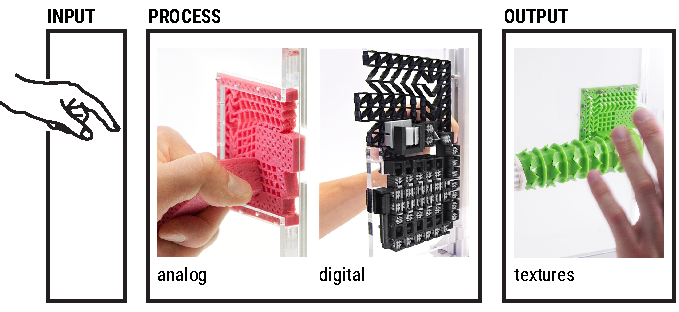
\includegraphics[width=\textwidth]{chapters/introduction-FIG/1-input-process-output.pdf}
    \caption[Short figure name.]{Metamaterial devices can process users' input and output to them again, thereby implementing an \textit{input-process-output} system without electronics, but purely within the material structure.
    \label{fig:1-overview-input-process-output-model}}
\end{figure}

Figure \ref{fig:1-overview-input-process-output-model} illustrates the core areas that we investigated in this thesis: we show (1) how we process \textit{analog} information in the context of metamaterials that transform forces and movements input by the user into a different set of forces and movement (i.e., mechanisms, (2) a system of cells that process information \textit{digitally}, and (3) cells that output information to the user or interface with the environment by appropriating dynamic textures.

Since designing such complex systems of cell structures is difficult, we additionally focus our work on providing accessible software to enable users to create such metamaterial devices.

% \begin{enumerate}
%     \item We integrate mechanisms within the material structure. Such metamaterial mechanisms consist of a single block of material the cells of which play together in a well-defined way in order to achieve macroscopic movement. This allows us to implement, e.g. a door latch, pliers, or a drawing machine from only one piece, without moving parts. 
    
%     \item Going beyond mechanical functions, we explore how to embody mechanical computation into 3D printed objects, i.e., without electronic sensors, actuators, or controllers typically used for this purpose. We demonstrate interactive objects based on this concept, such as a combination lock that are printed in one piece.
    
%     \item To further enhance 3D printed objects, we use metamaterials to change their outside. Such metamaterial textures can perform a controlled transition between two or more textures to allow designers to shape how objects interact with the environment and with the tactile sense of the user. 
% \end{enumerate}

% since we want to create interactive objects, we generally let the user provide input to our systems. 



\subsection{Processing analog signals}
We push the concept of metamaterials further by creating metamaterials that implement devices that transform input forces and movement into a desired set of output forces and movement---also known as mechanisms. Such metamaterial mechanisms consist of a single block of material the cells of which play together in a well-defined way in order to achieve macroscopic movement.

Figure \ref{fig:2-overview-metamaterial-mechanisms} shows an example of a metamaterial mechanism: a door latch mechanism. Our metamaterial door latch transforms the rotary movement of its handle into a linear motion of the latch. The key to transforming analog input are our shearing cells as they are only able to shear when subjected to an external force and thereby apply a controlled force to their neighboring cells.  While the traditional door latch mechanism consists of several parts, including an axle, bearings, springs, etc., the metamaterial door latch in Figure \ref{fig:2-overview-metamaterial-mechanisms} consists of a single block of material, as it is groups of cells inside the object that perform the mechanical function.
% The key element behind our metamaterial mechanisms is a specialized type of cell, the only ability of which is to shear. 

\begin{figure} [h] %[h!|H]
    \centering
    % 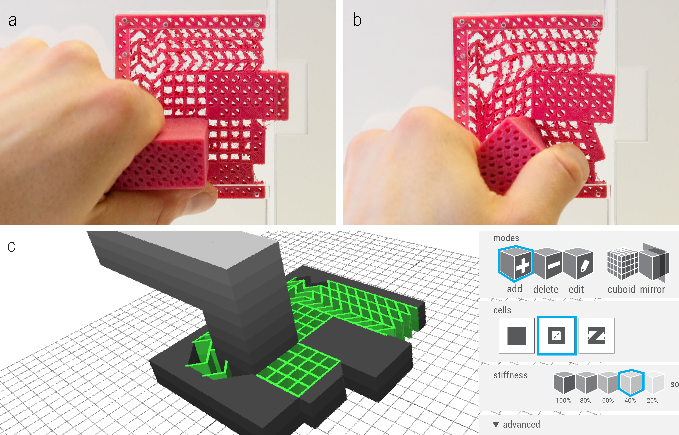
\includegraphics[width=0.85\textwidth]{chapters/introduction-FIG/2-overview-metamaterial-mechanisms.pdf}
    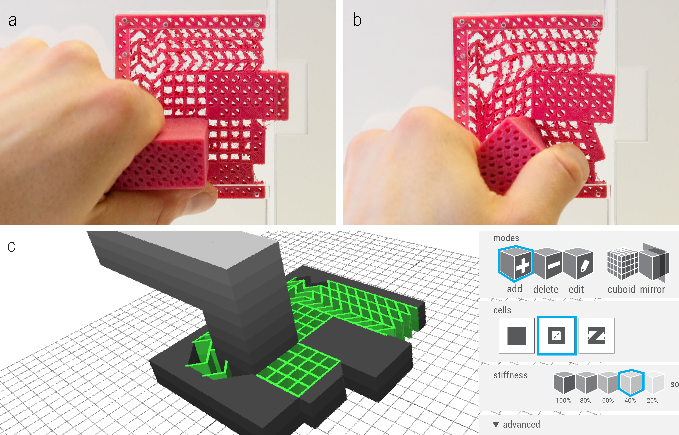
\includegraphics[width=1\textwidth]{chapters/introduction-FIG/2-overview-metamaterial-mechanisms.pdf}
    \caption[Short figure name.]{(a) This door latch demonstrates a metamaterial device that transforms user input, i.e., pushing down the handle, (b) to pulling the latch inwards. (c) We developed a custom editor to assist their design.
    \label{fig:2-overview-metamaterial-mechanisms}}
\end{figure}


The design of metamaterial mechanisms is highly challenging and the extent of mechanisms that can be realized with metamaterials remains unclear. 
We show in Figure \ref{fig:2-1-understanding-constraint-interaction} how a small change can lead to a vastly different output. 
The reason is that a mechanism consists of many cells that are interconnected and impose constraints on each other, the behaviour of the cell structure is unobvious and non-linear. 
To enable novice users to design such metamaterial mechanisms, we implemented a computational design tool takes user-drawn paths as input and optimizes the cell configuration which implements the transformation. 

To achieve this, we dig deeper into the underlying topological constraints of such cell structures and their influence on the resulting mechanism. 
We find that by representing the constraints as a graph we can easily distinguish unique cells configuration. 
For example, Figure \ref{fig:2-1-understanding-constraint-interaction} illustrates that one cell can prevent 7 cells from shearing such that any permutation within these 7 cells creates the same output. 
We bypass these $2^7 = 128$ configurations by only operating on the constraint graph (i.e., merging and splitting connected components), which reduces our search space by several orders of magnitude and ultimately enables such an automatic tool.

% We present an abstraction of the underlying cell structures as a constraint graph, which informs the design of metamaterial mechanisms. For example, we discover that non-linear mechanical transformations can be realized. Based on these findings, we contribute a computational design tool that automatically creates a metamaterial mechanism from user-defined input and output motion paths. This tool is only feasible, because our constraint graph representation highly reduces the search space of possible arrangements of cells. 

\begin{figure} [h] %[h!|H]
    \centering
    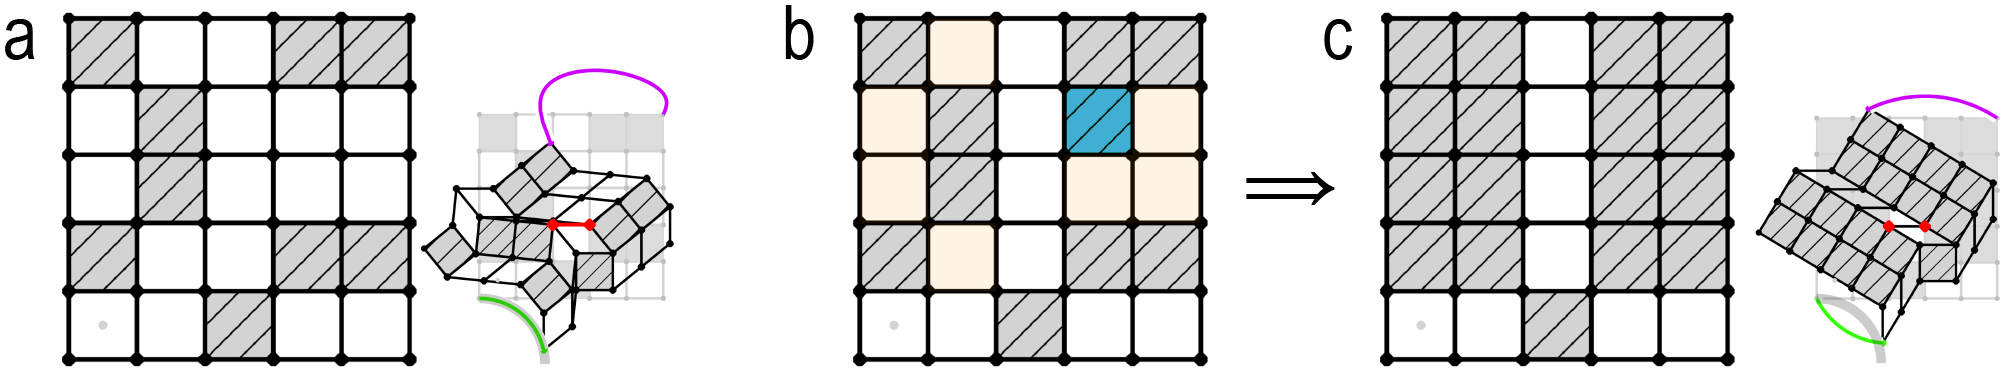
\includegraphics[width=1\textwidth]{chapters/introduction-FIG/2-1-understanding-constraint-interaction.png}
    % 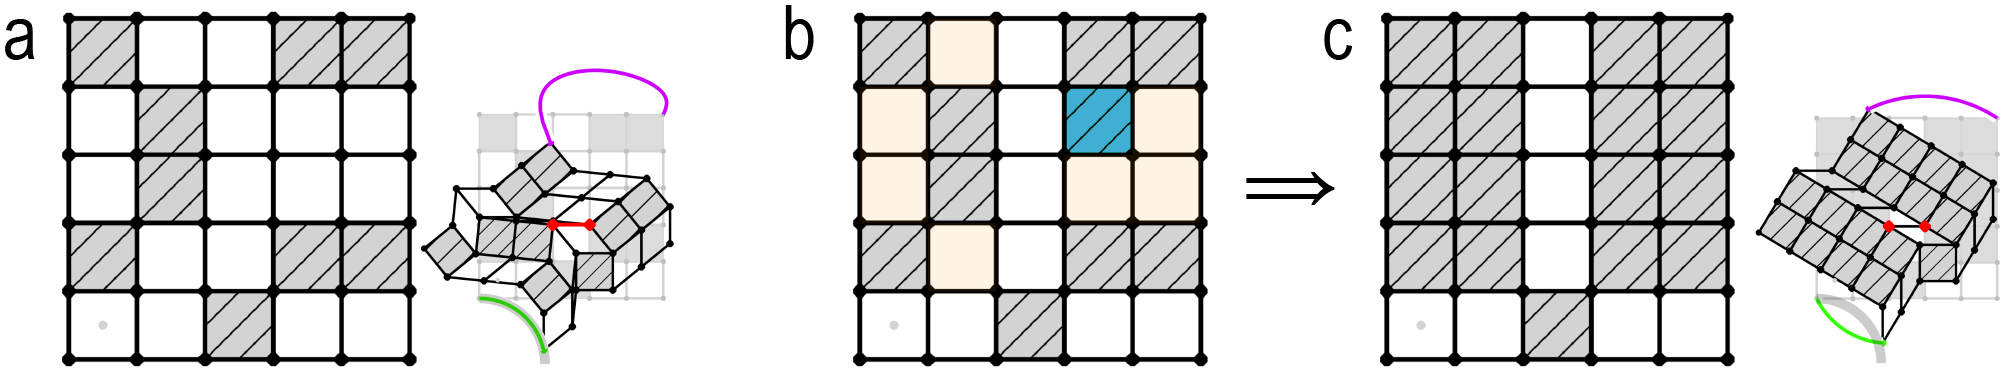
\includegraphics[width=0.85\textwidth]{chapters/introduction-FIG/2-1-understanding-constraint-interaction.png}
    \caption[Short figure name.]{(a) In this example, (b) setting one cell rigid (c) prevents 7 cells from shearing, which changes the output drastically. (c) The green input path from (a) cannot be followed anymore.
    \label{fig:2-1-understanding-constraint-interaction}}
\end{figure}


\subsection{Processing digital signals}

Such analog machines, however, are limited in terms of complexity. As forces are passed on from one cell to the next, they are damped and the activation energy dissipates, causing the mechanical ``signal" to decay. This limits the number of mechanisms that can be concatenated and therefore the complexity of the machine. While this decay can be minimized, it can never be eliminated. This motivated the question `Can we create metamaterials that process digital input, which have no signal decay?' 

To explore this concept, we introduce a new type of cell that propagates a digital mechanical signal, i.e., it counteracts signal decay and thus allows signals to pass through an arbitrary number of cells. Our cell embeds a bistable spring, which discharges when triggered. The resulting impulse triggers one or more neighboring cells, resulting in signal propagation. We extend this basic cell to allow users to implement combinational circuits within 3D printed metamaterial objects. To illustrate this concept, Figure \ref{fig:3-overview-digital-metamaterials} shows a combination lock implemented using digital metamaterials. We contribute 3D printable cells that process signals and make this concept of digital metamaterials accessible to users by extending our specialized 3D voxel-style editor.

\begin{figure} [h] %[h!|H]
    \centering
    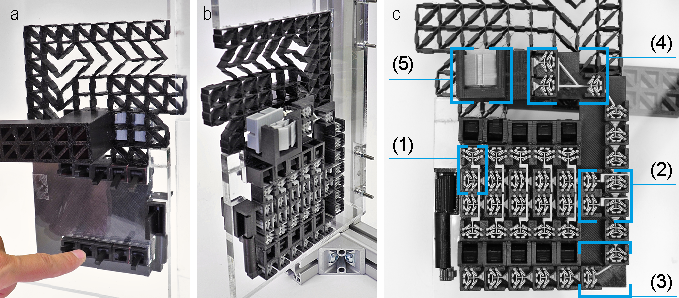
\includegraphics[width=1\textwidth]{chapters/introduction-FIG/3-overview-digital-metamaterials.pdf}
    % 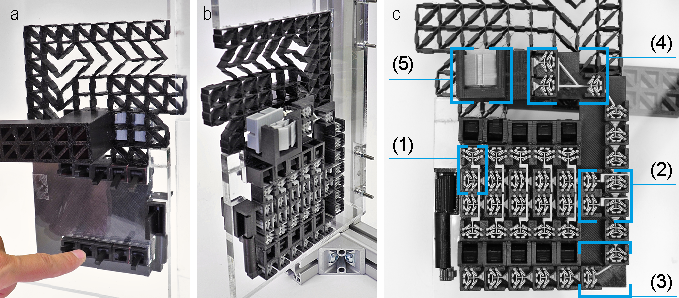
\includegraphics[width=0.85\textwidth]{chapters/introduction-FIG/3-overview-digital-metamaterials.pdf}
    \caption[Short figure name.]{(a) This combination door lock consists of cells that process the code and (b) only unlock the latch if users input the correct code. (c)~Internally, the lock consists of that implement (1) signal validation, (2) logic gates, (3) signal routing, (4) bifurcation, and (5) amplification.
    \label{fig:3-overview-digital-metamaterials}}
\end{figure}


\subsection{Output to the user and the environment}

After investigating two types of metamaterial structures that process information input by the user, we shifted our focus to create metamaterials that \textit{output} to the user. 

We apply the main idea behind metamaterials, i.e., subdivision into a large number of cells and customization on a per-cell basis, to the outsides of 3D printed objects. We introduce metamaterials that undergo a controlled transformation when an external force is applied, allowing users to transition between multiple dynamic textures after fabrication. The resulting metamaterial textures allow designers to shape how the object interacts with the environment and with the tactile sense of the user. Figure \ref{fig:4-overview-textures} shows an example. This door handle transforms its outside, allowing the person behind the door to set three levels tactile messages for everyone trying to enter. The inside of the door handle consists of a grid of cells, which controls how the texture on the object's surface will be formed. 
%We integrated our textured handle with our metamaterial door latch.

\begin{figure} [h]
    \centering
    \includegraphics[width=1\textwidth]{chapters/introduction-FIG/4-overview-textures--2.pdf}
    % 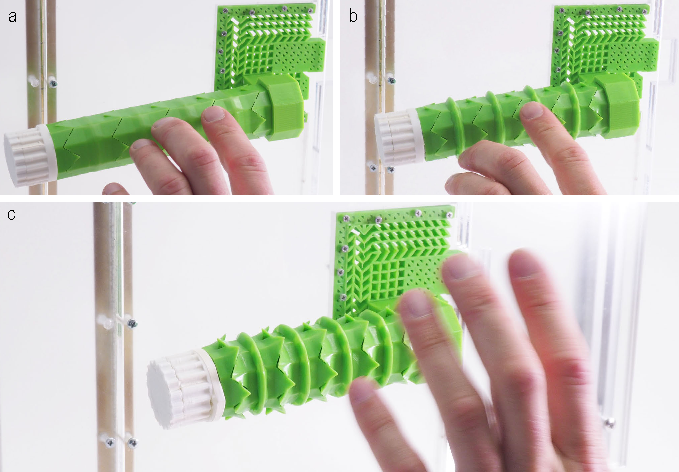
\includegraphics[width=0.85\textwidth]{chapters/introduction-FIG/4-overview-textures.pdf}
    \caption[Short figure name.]{When an external force is applied, metamaterial textures undergo a controlled transformation. This door handle, transforms (a) from flat (b) to rippled (c) to spiky, allowing the person behind the door to set a tactile message with three levels of enter/busy/do not enter messages for visually impaired or sighted users trying to enter.
    \label{fig:4-overview-textures}}
\end{figure}



\section{Contributions}

\textit{The concept of metamaterial devices.} \enspace The main contribution of this thesis is that we apply a radically different thinking to metamaterials. While this emerging field already demonstrated that materials with extreme properties can be engineered by designing their cell structure, we push this further and argue that we can engineer material properties to function as \textit{devices}. 

\textit{Applications and design space.} \enspace We investigated the potential impact and relevance of such metamaterial devices by exploring and building tangible prototypes that can be experiences. These demonstrations inform the potential design space for such devices.

\textit{Cell designs.} \enspace We also contribute a set of cells that enable the realization of metamaterial devices. Our cells include cells that enable a well-defined movement for transmitting forces between cells, they include cells that enable the processing and validation of digital signal and cells that change their outside to interface with the user and the environment.

\textit{Software.} \enspace Lastly, to enable users to create such metamaterial devices, we contribute easily accessible\footnote{open source editor for Metamaterial Mechanisms: \url{https://github.com/jfrohnhofen/metamaterial-mechanisms}} software tools that encapsulate our findings. Our software contains automatic generation of cell assemblies for novice users yet allows experts to freely edit their devices.



\section{Structure of this thesis}

%The structure of this thesis is straight-forward. 
We first give the reader a deeper insight into the current state of the art regarding digital fabrication and metamaterials in Chapter~\ref{chapter:related-work}. Then, in Chapter~\ref{chapter:analog-metamaterials}, we introduce the concept of metamaterial mechanisms. We dive deeper into the structural properties of metamaterial mechanisms in Chapter~\ref{chapter:Understanding-metamaterial-mechanisms}, where we also present a computational design tool that automates the generation of metamaterial mechanisms. We then move on to detailing the structures that enable digital metamaterial devices in Chapter~\ref{chapter:digital}, before explaining how to output to the user by appropriating dynamic textures in Chapter~\ref{chapter:textures}. 
In each chapter, we demonstrate the software that enables users to create such metamaterial devices. 
% In Chapter \ref{chapter:software}, we demonstrate the software that enables users to create such metamaterial devices. 
Lastly, Chapter~\ref{chapter:conclusion} concludes this thesis by discussing the work on a broader level. Since the concept presented in this thesis is novel, it opens up future directions of research, which we  identify and discuss to leave the reader with more food for thought. 
%Lastly, Chapter~\ref{chapter:conclusion} concludes this thesis by discussing the work on a broader level. Since the concept presented in this thesis is novel it opens up future directions of research, which we will identify and discuss in the end of this thesis to leave the reader with more food for thought.



















% something about 3D printers, layer by layer, arrange matter freely in space. 3D printers are solidifiers of digital geometry. Promise the 3rd revolution in manufacturing [economist] and in industrial sense it is getting there [Sculpteo]. but personal fabrication not there, becuase CAD tools are hard to use and hardware is not super reliable. this is why researchers investigate systems.

% % originally, fabrication was mostly concerned iwth the outside; decorative objects but also functional objects of simpler shape (e.g. cast). also due to the fact that 3D printing also comes with their limitations such as speed and support material, thus is also still in development. And designing the shapes also needs some sotware skill. Therefore working on shapes which is the most fail-safe in hardware and software sense, makes sense.  



% % \section{The promise of 3D printing}

% % 3d printing is promising because it can arrange matter freely in space. Does so by a layer by layer approach, thus can make complex geometry without many parts to assemble. other technologies could not, such as laser cutting is 2D and milling needs space for the head to travel.

% % Expected that everyone can make everything. Has printer at home, since they are cheap now. This has not happened yet, mainly because sotfware skill required to design the object and the printers still fail. Researchers work on making 3D printing more accessible and platforms provide models.


% % how great, industrial revolution, slowly happening [Sculpteo]. Personal fabrication less due to 




% % Personal fabrication machines, such as 3D printers, allow users to make custom objects. While early work on 3D printing revolved around designing the outside of such objects [e.g., 35], recently researchers started exploring 3D printing as a means to design the inside of objects. Applications include moving objects’ centers of gravity so as to make them stand [23] or spin [3].

% % Pushing this further, researchers created objects that consist internally of a large number of 3D cells arranged on a regular grid. Since each cell is designed to perform a specific deformation [20], objects that entirely consist of such cells literally offer thousands of degrees of freedom. Such structures are also known as mechanical metamaterials. Metamaterials are artificial structures with mechanical properties that are defined by their usually repetitive cell patterns, rather than the material they are made of [4, 21].

% % Based on this concept, researchers have created objects with unusual behaviors, such as metamaterials that collapse abruptly when compressed [26, 31], that shrink in two dimensions upon one-dimensional compression [28], or objects that mix layers of soft and hard cells in order to emulate different materials [5].


% \subsubsection{From the outside}  
% % \subsubsection{From outside shape}  
% The recent rise of widely accessible fabrication machines, such as 3D printers or laser cutters, generated interest in non-experts to create and design their own devices. Their strive towards a future of personal- rather than mass-fabrication is supported by HCI researchers, who investigate techniques to directly interact with the machine \cite{Mueller2012a}, use real-world objects for content creation \cite{Weichel2014, Weichel2015} or embed mechanisms \cite{Zhang2017} and electronics \cite{Weichel2013, Ledo2017}. These were mainly concerned with creating the outside shape of 3D models.

% \subsubsection{To the inside} 
% % \subsubsection{To static internal structure} 

% % JUST EXPLAIN THESE WORKS IN MORE DETAIL?
% 3D printing technology, however, is unique in that is allows users to freely arrange matter in space. \todo{add netfabb and so} Researchers used this property to generate internal structures that, e.g., optimize the strength to weight ratio of 3D objects \cite{Lu2014}, allow arbitrarily shaped objects to spin reliably \cite{Bacher2014a}, or to float in pre-defined poses \cite{Prevost2016}.

% % \subsubsection{To engineered materials} 
% \subsubsection{To engineered microstructures} 
% Pushing this further, researchers created objects that consist internally of a large number of 3D cells arranged on a regular grid. Since each cell is designed to perform a specific deformation \cite{Overvelde2012a}, objects that entirely consist of such cells literally offer thousands of degrees of freedom. Such structures are also known as mechanical metamaterials. Metamaterials are artificial structures with mechanical properties that are defined by their usually repetitive cell patterns, rather than the material they are made of \cite{Bertoldi2017, Christensen2015, Paulose2015}.

% \todo{add overview of what metamaterials can do, add schumacher}


% % \section{Metamaterial devices: \\defined by their internal structure}
% \section{Metamaterial devices}

% So far, metamaterials have been understood as materials. The main contribution of this thesis is that we want to think of them as \textit{devices.}

% % \todo{add some diagramm that shows this distinction between metamaterials and devices}


% In this dissertation, we push the concept of metamaterials further by creating 3D printed structures inside objects that can process users' input and output to them again, thereby implementing an \textit{input-process-output} system without electronics, but purely within the material structure. The key benefit of our approach is that the resulting objects can be 3D printed from a single material and in one piece and thus do not require assembly.

% % \begin{figure} [h] %[h!|H] 
% %     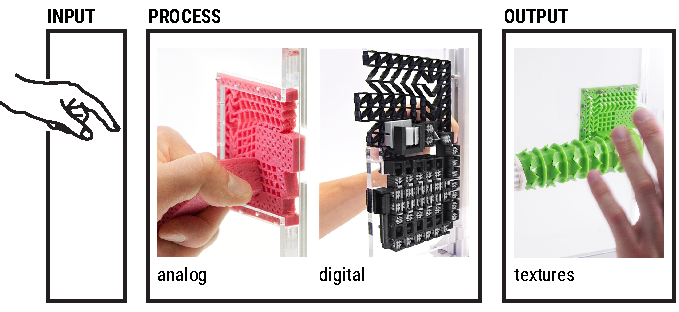
\includegraphics[width=\textwidth]{chapters/introduction-FIG/1-input-process-output.pdf}
% %     \caption[Short figure name.]{Metamaterial devices can process users' input and output to them again, thereby implementing an \textit{input-process-output} system without electronics, but purely within the material structure.
% %     \label{fig:1-overview-input-process-output-model}}
% % \end{figure}

% We contributed cell structures and computational tools that enable users to create 3D printed metamaterial objects capable of processing analog and digital input, as well as to output to the user. 

% \begin{enumerate}
%     \item We integrate mechanisms within the material structure. Such metamaterial mechanisms consist of a single block of material the cells of which play together in a well-defined way in order to achieve macroscopic movement. This allows us to implement, e.g. a door latch, pliers, or a drawing machine from only one piece, without moving parts. 
    
%     \item Going beyond mechanical functions, we explore how to embody mechanical computation into 3D printed objects, i.e., without electronic sensors, actuators, or controllers typically used for this purpose. We demonstrate interactive objects based on this concept, such as a combination lock that are printed in one piece.
    
%     \item To further enhance 3D printed objects, we use metamaterials to change their outside. Such metamaterial textures can perform a controlled transition between two or more textures to allow designers to shape how objects interact with the environment and with the tactile sense of the user. 
% \end{enumerate}

% \todo{and because designing 3D geometry is tricky, as said before, we provide software for these complex metamaterial devices}

% \todo{shorten subsequent sections!}

% \subsection{Processing analog signals}

% In this work, we push the concept of metamaterials further by creating objects that allow for controlled directional movement. This allows users to create objects that perform mechanical functions. Our objects thereby implement devices that transform input forces and movement into a desired set of output forces and movement—also known as mechanisms.

% Figure \ref{fig:2-overview-metamaterial-mechanisms} shows an example of a metamaterial mechanism: a door latch mechanism. Its interior is a regular grid of 3D cells; however, the cells are of different types. Applying a force causes the cells to deform in a controlled way, thereby performing the intended mechanical function. In the example, rotating the door handle causes the cells inside of the object to deform, ultimately pulling the latch towards the left and thereby unlocking the door.

% \begin{figure} [h] %[h!|H]
%     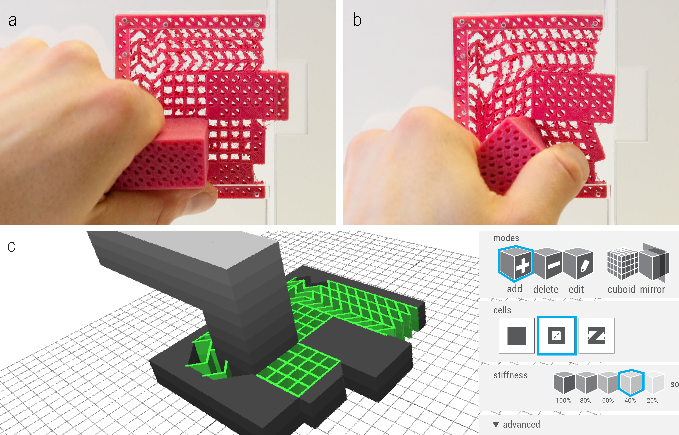
\includegraphics[width=\textwidth]{chapters/introduction-FIG/2-overview-metamaterial-mechanisms.pdf}
%     \caption[Short figure name.]{(a) This door latch is implemented as a metamaterial mechanism; it consists of a single block of material based on a regular grid of cells that together implement handle, latch, and springs. (b) Turning the handle causes the central hinge array to deform and to pull the latch inwards, which unlocks the door. (c) We created this mechanism in our custom editor. Here, we placed two hinge arrays that mechanically couple the handle to the latch, and cells that couple to the doorframe.
%     \label{fig:2-overview-metamaterial-mechanisms}}
% \end{figure}

% While most of the object consists of rigid cells (cells that are reinforced with a diagonal), the object also contains several rectangular regions of cells that lack such a diagonal reinforcement. These are the key to creating mechanisms, as they are able to deform in a very specific way: when subjected to an external force, these cells shear and thereby apply a force to their neighboring cells. 

% Metamaterial mechanisms are simple. While the traditional door latch mechanism consists of several parts, including an axle, bearings, springs, etc., the metamaterial door latch in Figure \ref{fig:2-overview-metamaterial-mechanisms} consists of a single block of material, as it is groups of cells inside the object that perform the mechanical function.

% % While mechanical engineers typically generate metamaterials by scripts [e.g., 21], allowing users of different backgrounds and expertise to create mechanisms requires a dedicated design/engineering process that we argue is best performed by means of an interactive editor. Figure \ref{fig:2-overview-metamaterial-mechanisms}c shows the custom 3D editor we created specifically to allow users to create and modify metamaterial mechanisms. It contains a range of functions that help users assemble specialized cells into basic mechanisms and to assemble such basic mechanisms into more complex mechanisms and simple machines. Using this editor, we have created a series of demo objects including the door latch, a Jansen walker, or a functional pair of pliers. Our examples were printed on a consumer 3D printer (Ultimaker 2+) using a single material.


% \subsection{Processing digital signals}

% Such analog machines, however, are limited in terms of complexity. As forces are passed on from one cell to the next, they are damped and the activation energy dissipates, causing the mechanical ``signal" to decay. This limits the number of mechanisms that can be concatenated and therefore the complexity of the machine. While this decay can be minimized, it can never be eliminated. 

% Therefore, in this work, we explore how to extend this concept towards digital mechanisms, which have no signal decay. Combining metamaterial mechanisms with concepts from mechanical computing and mechanical signal propagation \cite{Raney2016, Nadkarni2014}, we introduce a new type of cell that propagates a digital mechanical signal, i.e., it counteracts signal decay and thus allows signals to pass through an arbitrary number of cells. 
% We introduce a new type of cell that propagates a digital mechanical signal using an embedded bistable spring. When triggered, the embedded spring discharges and the resulting impulse triggers one or more neighboring cells, resulting in signal propagation. We extend this basic cell to allow users to implement combinational circuits within 3D printed metamaterial objects by contributing signal routing, bifurcation, amplification, validation, and logic gates based on 3D printable cells. 

% \begin{figure} [h] %[h!|H]
%     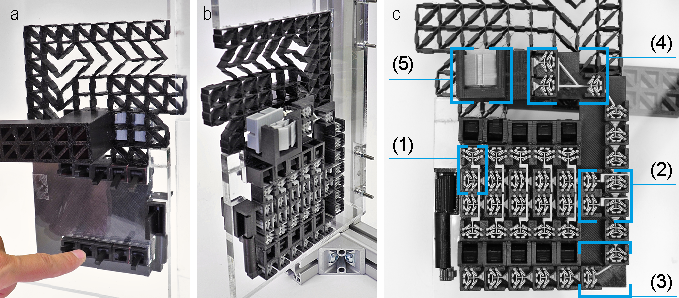
\includegraphics[width=\textwidth]{chapters/introduction-FIG/3-overview-digital-metamaterials.pdf}
%     \caption[Short figure name.]{(a) This combination door lock is implemented as a digital mechanical metamaterial, i.e., a single block of material based on a regular grid of cells. It allows users to input a numeric code, (b) it processes the code, checks its correctness, and unlocks the latch. (c) Internally, the lock consists of an array of cells that transmit and process a mechanical signal.
%     \label{fig:3-overview-digital-metamaterials}}
% \end{figure}

% To illustrate this concept, Figure \ref{fig:3-overview-digital-metamaterials} shows a combination lock implemented using digital metamaterials. The aforementioned shearing cells of the door latch mechanism are blocked by bolts. These bolts are retracted by the digital combination lock only if the user entered the correct 10-digit code. To input the code, users tap one of the 10 digit buttons on the front and push the ‘open’ button, which sets off three signal transmission lines simultaneously; two of which run through the digit evaluation units (Figure \ref{fig:3-overview-digital-metamaterials}c (1)) and set the state of the AND gate (2), which evaluates the correctness of the two rows of digits input by the user. The third signal transmission line is routed (3) from the bottom left towards the right, around the corner, and upwards where the signal is bifurcated (4). This allows triggering a double-sized amplifier cell (5) that actuates the bolts to unblock the door.

% To allow expert users to create and fabricate objects from digital metamaterials, we implemented a specialized 3D voxel-style editor, which is based on the editor for metamaterial mechanisms. The main intent is to allow users to draw signal paths and verify them within the editor. We support users by allowing them to enter simple logic functions, which our editor converts to cell arrangements that implement that function.


% \subsection{Output to the user and the environment}

% In this work, we apply the main idea behind metamaterials, i.e., subdivision into a large number of cells and customization on a per-cell basis, to the outsides of 3D printed objects. The resulting metamaterial textures allow designers to shape how the object interacts with the environment and with the tactile sense of the user.

% We introduce metamaterials that undergo a controlled transformation when an external force is applied, allowing users to transition between multiple dynamic textures after fabrication. Figure \ref{fig:4-overview-textures} shows an example. This door handle transforms from flat to rippled to spiky, allowing the person behind the door to set three levels of enter/busy/do not enter tactile messages for everyone trying to enter. We integrated our textured handle with our metamaterial door latch.

% \begin{figure} [h]
%     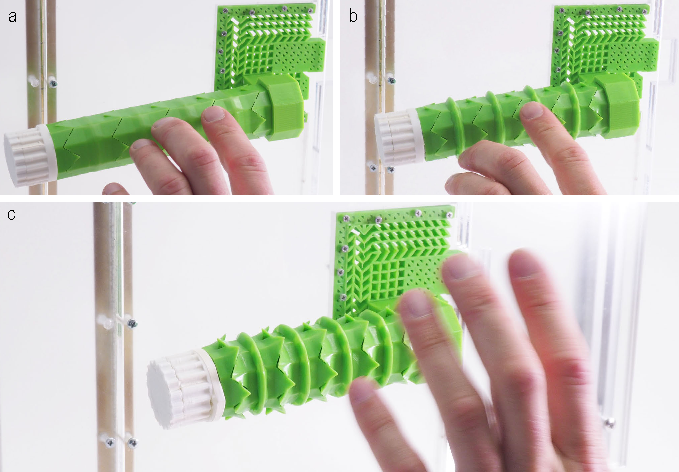
\includegraphics[width=\textwidth]{chapters/introduction-FIG/4-overview-textures.pdf}
%     \caption[Short figure name.]{When an external force is applied, metamaterial textures undergo a controlled transformation. This door handle, for example, transforms (a) from flat (b) to rippled (c) to spiky, allowing the person behind the door to set a tactile message with three levels of enter/busy/do not enter messages for visually impaired or sighted users trying to enter.
%     \label{fig:4-overview-textures}}
% \end{figure}

% The inside of the door handle consists of a grid of cells, which controls how the texture on the object's surface will be formed. We call the underlying cells fold cells. Each cell implements a simple mechanism that transforms horizontal compression into vertical deformation, i.e., it folds upwards when compressed creating a tactile bump. Hence, chaining multiple of these cells allows popping out a texture on the surface of the object. 

% % Beyond this door handle example that uses textures to provides tactile feedback to visually impaired users, such transformable textures allow users to make objects that are adaptable to a specific context such as a shoe sole that transforms from flat to treaded to adapt to weather conditions, or a configurable bicycle grip for exploring parameters during rapid prototyping of textures.

% We present an editor that assists users in creating metamaterial textures interactively by arranging cells, applying forces, and previewing their deformation. Users can achieve a variety of textures by setting the parameters of fold cells, such as hinge offset, width and wall thickness, etc. After having combined their cells, they interactively simulate how the cells deform under continuous compression. Finally, this geometry is exported into a 3D printable .stl file.


% \section{Structure of this thesis}
% \todo{summarize structure}

\chapter{Related work}
\label{chapter:related-work}

% Advances in digital fabrication and the growing availability of fabrication machines accelerated the research in many areas. They allowed the exploration of custom 3D objects that can sense user input,  

% recent advances in fabrication technology enabled lots of stuff; availability of simple printers (FDM, SLA) people making stuff, multi-material printers enabled customized stuff like prosthetics, nanoscale printers enabled even new materials. this is the related work that this work builds on.

Our work builds on previous work in interactive personal fabrication,  on techniques that modify the internal structure of 3D printed objects, multi-material printing, and in particular on mechanical metamaterials.





\section{Interactive systems for fabrication}

Personal fabrication devices such as 3D printers and laser cutters allow users to fabricate personalized physical objects. Researches presented interactive systems that ease the process of designing static objects, creating interactive objects and interacting directly with the machine.

% Besides fabricating common decorative objects from rigid plastic, researchers presented systems for creating interactive objects, or interacting directly with the machine \cite{Baudisch2017}.

% researchers showed how to fabricate a variety of objects, such as printing soft teddy bears \cite{Hudson2014}, optical sensors \cite{Willis2012}, or loudspeakers \cite{Ishiguro2014}.


\subsection{Designing 3D models}

% As the market for additive manufacturing (3D printing) is growing \cite{Sclupteo2018}, not only the hardware, but also the software to create the 3D model is 

The first step to fabricating custom object using 3D printing is to design the digital 3D model. There are many tools to do so, the currently most popular tools include easy-to-use CAD systems such as Tinkercad or SketchUp, expert tools such as SolidWorks and Inventor, or parametric modelling tools such as Rhinoceros or openSCAD \cite{imaterialise2017}. 

Researchers in HCI and computer graphics investigated systems to ease the process of creating 3D models, e.g., by implementing sketching-based interfaces for simple toy-like models \cite{Igarashi1999}, or for more complex models such as planes  \cite{Tsang2004, Bae2008, Bae2009}. Going beyond creating only the virtual model, researchers integrated the fabrication of the physical model into the design system by simulating the, e.g., sown plush model \cite{Mori2007} or stability of the interlocked laser cut chair \cite{Saul2011}. In general, making 3D objects from laser cut 2D shapes by interlocking them orthogonally is popular, since laser cutting is simpler and faster than 3D printing. Researchers support these benefits of laser cutting and develop systems that create laser cut pieces from a 3D model \cite{Hildebrand2012, McCrae2014}.

More complex mechanical object and articulated figures, rather than the aforementioned static object, require special items such as joints \cite{Ureta2016} and user-defined motion-ranges \cite{Megaro2014}. LinkEdit \cite{Bacher2015} allows users to edit the moving linkage as to satisfy space constraints. Megaro et al. \cite{Megaro2015} take this concept event further and implement as systems that generates stable motions for legged robots of arbitrary designs and exports the 3D-printable geometry.


\subsection{Interacting with the machine}

The traditional workflow for fabricating physical models consists of users creating the 3D model at their computer, then sending the model to the fabrication machine and waiting until the machine is done. In case of 3D printing, this could mean waiting for hours -- days until the object is finished. However, when fit or ergonomics is an issue, this process is not feasible as it does not allow for iterating over the design. Achieving a good fit between the fabricated object and external object, Weichel et al. \cite{Weichel2014, Weichel2015} proposed using the target objects in an AR environment during the modeling process. Gannon et al. \cite{Gannon2015} investigated a fabrication system that allows users to design directly on their skin for body-fit items such as casts.

The availability to iterate over a design is crucial for rapid prototyping, which is why researcher investigated how to decrease the time between iterations. This includes integrating building blocks \cite{Mueller2014}, printing only low-fidelity previews \cite{Mueller2014a}, or destroying only part of the model for updating instead of reprinting the whole part \cite{Teibrich2015}. \textit{On-the-Fly Print} \cite{Peng2016} even allows users to design 3D models digitally while having a low-fidelity physical wireframe model printed in parallel. 

% \cite{Roumen2016} Mobile Fabrication

Going beyond quick iterations cycles, researchers investigated interactive systems that allows users to interact directly on the machine. This powerful concept was first instantiated by a foam extruder that was integrated with a touch-table \cite{Willis2011a}. Extending this concept, Müller et al. investigated systems that allow users to draw mechanical parts directly onto the laser cutter \cite{Mueller2012a, Mueller2013}. This makes the machine a collaborator, which was taken further by systems, such as \textit{FormFab} \cite{Baudisch2017} or \textit{RoMA} \cite{Peng2018} that enable a collaboration with a robotic arm for fabrication.

Working directly on the machine also presents another way to creating the digital 3D model. \textit{D-Coil} \cite{Peng2015a}, for example, allows users to create a physical model using a handheld extruder and creates the digital model by tracking the extruder's movements. 

% \cite{Weichel2015} - ReForm: Integrating Physical and Digital Design through Bidirectional Fabrication
% \cite{Follmer2012} - KidCAD


\subsection{Interactive objects and unconventional materials}

Researchers did not only investigate how to create interactive fabrication systems, but also how to fabricate interactive objects. One way is to achieve interactive objects is to create systems that allow users to define space inside the object to include electronic components, such as microcontroller boards \cite{Weichel2013}, mobile devices \cite{Ledo2017}, or electro-luminescent wire \cite{Savage2014}. Using conductive filaments, users can add capacitive sensing capabilities to their 3D printed objects \cite{Schmitz2017, Burstyn2015, Vasilevitsky2016, Katsumoto2013}. Researchers also integrated other sensing technologies into 3D printed objects, including pneumatic sensing \cite{Savage2014, Slyper2012, He2017}, acoustic sensing \cite{Savage2015}, or optical sensing \cite{Willis2012, Savage2013}.

Commonly available materials for 3D printers include plastics, resins, metals and plaster; and for laser cutters wood, paper, acrylic, and metal. Researchers go beyond these materials and invented machines that go beyond these materials. They demonstrated systems that can produce 3D objects from stacks of paper \cite{Oh2018}, that can create soft objects from wool \cite{Hudson2014} or felt \cite{Peng2015}, that integrate fabric with plastics \cite{Rivera2017, Perez2017}, or print with biological material \cite{Wang2016, Yao2015a}.

% not using, but creating interesting hair-like material: Cilllia \cite{}
% Muth,Lewis14 Embedded 3D Printing of Strain Sensors within Highly Stretchable Elastomers

% \subsubsection{Fabricating interactive objects}







\section{Altering the material distribution}

Changing the material distribution inside 3D objects for manipulating objects' properties. This includes changing the density of static objects, distributing rigid and soft materials to change how objects' deform or to make them fold from 2D to 3D structures.

\subsection{Static internal material distribution}
Researchers in HCI and computer graphics explored how to define the behavior of printed objects. In particular they optimized the rigid internal structure of objects in order to optimize the object’s strength-to-weight ratio depending on predefined static loads \cite{Lu2014, Chen2018, Wu2016}. By defining void areas inside a 3D object, researchers effectively move the object’s center of gravity in order for unbalanced shapes to stand \cite{Prevost2013}.

Similar approaches are also effective for dynamic movements. For example, void areas on the inside of objects can be optimized in order to allow arbitrary objects to spin \cite{Bacher2014a}. To give arbitrary shapes multiple stable poses, researchers integrated moving masses \cite{Prevost2016}, which even allows for stable poses while the object is floating in water.


% \subsection{Varying compliance by combining multiple materials}
\subsection{Defining how objects deform}

More complex fabrication processes allow to print with multiple materials and therefore to compliance and deformation as properties to engineer with. Multi-material 3D printers, such as the Objet Connex series, allows to deposit different materials at every voxel. 

\subsubsection{Localized compliance}
This allows mixing stiff and soft material arbitrarily throughout the object \cite{Kou2007}. By applying techniques such as dithering, highly personalized compliance distributions for, e.g., sockets of prosthetics \cite{Doubrovski2015}, can be realized. Another interesting application area of objects with localized compliance is to realistically model how organs feel, which can serve in the training of doctors. For this purpose, Zehnder et al. \cite{Zehnder2017} developed a computational approach to calculate the internal distribution of stiffer silicone within soft silicone as to resemble a specific feel on the outsite.

% (tools to create multi-material objects: VoxCAD, Vidimce, Spec2Fab, Foundry)
% multi-material printers even enable printing hydraulic machines, i.e., ... \cite{MacCurdy2016}.\\


\subsubsection{Reaching a target shape}
Optimizing the material distribution can be used to match a pre-defined target shape based on some simple actuation. For example, Skouras et al. \cite{Skouras2013a}, used multi-material printing to create articulated characters. They computed which voxels will be printed using stiff material and which using soft materials, taking into account some locations where the material will be pulled, to match the target shapes of a figure. {P{\'{e}}rez et al. \cite{Perez2015} also matched target shapes, but by optimizing a rod network from a single material. Such target-shape optimizations were also demonstrated for inflatable structures \cite{Skouras2012}, where the stretching of the material after inflation is taken into account. To control the resulting target shapes further, researchers printed rigid shapes onto pre-stretched material \cite{Perez2017, Guseinov2017}. The benefit of this approach is that the object is fabricated as a flat piece and only transforms into its target shape once the tension of the base material is released. 


\subsubsection{Shape-change and self-assembly}
Self-assembly builds on a similar concept, where objects are designed to be fabricated flat and to fold up into a 3D shape once they are actuated  \cite{Tibbits2014, Raviv2015}. Typical forms of actuation include pneumatic actuation, the use of thermally responsive or light absorbing or hydrophilic materials \cite{Geryak2014, VanManen2018}. 

Pneumatically actuated objects feature strategically placed pockets that are inflated after fabrication to transform from 2D to 3D \cite{Ou2016, Overvelde2016a}. This type of actuation, however, requires a compressor and some pipes, which is why researchers are interested in using materials with properties that are easier to actuate. Submerging objects in water is easy to do. Therefore, researchers layered hydrophobic and hydrophilic materials as an actuation mechanism \cite{Raviv2015, Wang2017}. Once the object is submerged in water, the hydrophilic material soaks up water and expands making the area bend. Placing such bending elements strategically allows for self-folding 3D objects.

Since actuation using water is very slow, researchers investigated thermally active materials \cite{Ge2014} such as shape memory polymers \cite{Yu2015}. Sandwiching a thermally active material between two layers of rigid materials allows controlling the bending angles and direction (mountain vs. valley fold) by generating parameterized gaps in the rigid material \cite{An2014}. The folding of complex shapes requires to take the sequence of folding of parts into to self-collisions, which Mao et al. \cite{Mao2015} solved by modifying the composition of shape memory polymers as to program the folding sequence of an object. Recently, these capabilities were made available for simple 3D printers using commonly available materials (TPU, PLA, paper) \cite{An2018, Wang2018}. 

Hawkes et al. \cite{Hawkes2010} introduced magnets that hold the 3D shape of their heat activated self-folding objects while Miyashita et al. \cite{Miyashita2015} build use magnet that is enclosed in the self folded object to enable remote actuation, thus acting like a simple robot. 

While thermally responsive materials are most common for self-assembly, researchers also investigated light absorbing materials as an actuation technique \cite{Tolley2013} and even biological materials \cite{Yao2015, Wang2017a}.

The benefits of such programmable, self-assembling objects span from easing packaging and transportation to remotely actuated robots \cite{Miyashita2015} that can even be ingested \cite{Miyashita2016}. Researchers are working towards entirely soft, autonomous robots \cite{Wehner2016}.

% based on origami: looking at geometry, non-idealized \cite{PerazaHernandez2016} Modeling and analysis of origami structures with smooth folds


\subsection{Monolithic mechanisms based on deformation}

Compliant mechanisms are deforming structures that by allow for implementing a mechanism placing flexures. While traditional mechanisms use very stiff (rigid) parts that are connected by hinges to transform motion or forces, compliant mechanisms consist of (mostly) one part with the hinging parts being very thin \cite{Howell2013}. Making the material thin increases its flexibility and allows for hinging behavior. Therefore, these parts are also known as flexures \cite{Trease2005}. Since the movement is performed by deformation there is virtually no friction, no need for lubrication, and thus for maintenance. Due to consisting of only one part, compliant mechanisms miniature well and are therefore commonly used in micro-electromechanical systems (MEMS) \cite{Gafford2014}.

To create such compliant mechanisms, researchers proposed topology optimization algorithms \cite{Sigmund1997a, Zhu2013, Zhu2014}, which allow for an abstract problem statement and return the material distribution on a voxel-level that implements a simple mechanism such as a gripper. However, topology optimization is also effective on a defined network of struts \cite{Mankame2004, Mankame2006, Saxena2005}. Recently, Megaro et al. \cite{Megaro2017} presented a system that converts a traditional linkage mechanism into complex compliant mechanisms (e.g., a hand with all joints).

% Interestingly, Rai et al. \cite{Rai2010} showed that partially compliant mechanisms, i.e., compliant mechanisms that incorporate some traditional hinges, are more stable than fully compliant or traditional mechanisms. To increase the 

% partially compliant mechanism better than fully compliant or rigid body \cite{Rai2010}.
% contact-aided (explain): 








\section{Engineering new materials}

Researchers in the disciplines of mechanical engineering and physics took such compliant structures to the micro- and nano-scale in order to engineer new materials. 

% \todo{ultimate goal: Synthesis Machine [Service2015]}

% \todo{fabrication techniques to achive this: \\
% VanAssenbergh2018: Nanostructure and Microstructure Fabrication: From Desired Properties to Suitable Processes \\
% Truby2016: Printing soft matter in three dimensions}

They create microstructures that define the material's properties. Such engineered material properties vary from ultra-lightweight structures over tuning of acoustic, optical, or electromagnetic wave lengths to mechanical properties such as shock absorption. We will focus on mechanical properties, as they are most relevant to this thesis. 

\subsection{Mechanical metamaterials}
Metamaterials are understood as artificial structures structures with properties that are defined by their usually repetitive cell patterns, rather than the material they are made of \cite{Bertoldi2017, Christensen2015, Paulose2015}.  

% ``Metamaterials are carefully structured materials---often consisting of periodically arranged building blocks---that exhibit properties and functionalities that differ from and surpass those of their constituent materials rather than simply combining them." \cite{Bertoldi2017}
% ``Metamaterials are man-made designer matter that obtains its unusual effective properties by structure rather than chemistry." [Christensen2015]
% ``Mechanical metamaterials are artificial structures whose unusual properties originate in the geometry of their constituents, rather than the specific material they are made of." [Paulose2015]

% \todo{foam example?}

Such `cells' can be designed and engineered to undergo a desired deformation. When many unit cells are connected on a larger grid, the individual deformations of the cells together form unprecedented macro-scale properties. Overvelde et al. \cite{Overvelde2012a, Overvelde2014} demonstrated the concept of metamaterials nicely: they showed how different unit cells, which were modeled as holes in a square with different shapes (circle, cross, star), influences the overall deformation when the material is compressed. And the overall deformation varies dramatically! 

% \todo{add image from my slides}

% \todo{Milton1995b}

Based on this concept of specifying the overall material properties by designing the internal structure, researchers developed many interesting materials, some of which we discuss in the following.

\subsubsection{Ultra-lightweight, strong materials} %Varying density, stiffness, or elasticity
Cells arranged on a regular grid were shown to be very successful in varying bulk material properties, i.e., properties that affect the entire material as opposed to localized properties. One interesting material property to engineer is its density. A traditional material that has amongst the highest strength-to-weight ratio are ceramics, however, at the same time they are very brittle. Meza et al. engineered a material that consists of octahedhedral-tetrahedral cells that are made of hollow ceramic beams \cite{Meza2014, Meza2014a, Montemayor2014, Zheng2014}. Only changing the geometry while still using ceramics to make the metamaterial allowed the material to compress up to 50\% and still recover. This means that these researchers successfully reduced the brittleness and created an ultra-lightweight yet strong material, which is relevant, e.g., for air- and spacecrafts. 

\textit{Hierarchical metamaterials. } Since such architected structures already showed such promising changes in properties, the researchers went further and applied them in a hierarchical manner \cite{Meza2015}. They made the beams within their nanolattices from self-similar structures and found that introducing hierarchy enables a combination ultra-lightweight and recoverability. Moreover, they observed a near-linear scaling of stiffness and strength with density, which promises for futher miniaturization.

\textit{Pentamode materials. } Milton \cite{Milton1995b} showed already in 1995 that such structures can be engineered to be rigid in one direction but compliant in another. One especially notable type of material are so-called pentamode materials. While they are rigid against compression in all directions they are very easy to shear, which makes them behave like solid fluids. Bückmann et al. later showed that such pentamode structures can be used as a `unfeelability cloak' \cite{Buckmann2014, Buckmann2015a}. They calculated the cells that surround an object as to feel like there was no object hidden in the material.

%stretchable (Choi2015, mesostructure, wrist band)\\


\subsubsection{Volume-changing materials (`auxetics')}

Another interesting material property is the expansion or contraction ratio. When conventional materials such as wood or metals are stretched, they compress in the orthogonal direction. However, in the late 1980ies, researchers suggested structures that would do the contrary, i.e., as a material is stretched vertically, it gets \textit{thicker} horizontally. The material effectively changes its volume. Such materials are known as auxetic materials or materials with a negative Poisson's ratio. After Almgren \cite{Almgren1985} demonstrated a mechanical structure made from rods, hinges and springs that has a negative Poisson's ratio, Lakes \cite{Lakes1987} suggested a monolithic 3-dimensional cell based on a similar structure.  

% Milton1992-Composite materials with poisson's ratios close to -1\\

These structures are known as re-entrant honeycombs and inspired many researchers to this day. It is a well researched topic due to the unusual nature of this auxetic property. There are several articles that review the developments of auxetic materials \cite{Ren2018, Kolken2017, Saxena2016, Christensen2015, Mir2014a} as well as an extended study of variations of cell geometries and the impact on the resulting Poisson's ratio \cite{AlvarezElipe2012}.

Auxetic materials can be achieved using re-entrant structures, as mentioned above, or by rotation. Re-entrant structures are, e.g., honeycombs where 2 opposite vertices of the hexagon are pushed towards the center of the structure. This causes them to push their neighboring cells horizontally outwards when they are pulled apart vertically, thus expanding in both directions. The same principle has also been shown on other re-entrant shapes, such as stars. The second mechanism is to arrange cells on a regular lattice and connect them at their corners, such that the cells (e.g., rigid squares, triangles, etc.) rotate around each other to expand in both directions \cite{Grima2000, Jiang2018}. Such auxetic materials can also be arranged in a hierarchical manner \cite{Seifi2017, Mousanezhad2015}, which allows for a better control over the degrees of freedom. These rotating cells can be produced by simply perforating sheets \cite{Shan2015a}. In fact, researchers in computer graphics used the auxetic property of rotating triangles to create 3D objects with spherical curvatures (doubly curved) from a perforated sheet \cite{Konakovic2016}.

Besides the just mentioned auxetic cells, there is also a very simple cell geometry that is auxetic. It is not obvious that it would be, since the cell is a simple square with a circular hole \cite{Mullin2007, Bertoldi2010}. Shim et al. \cite{Shim2013a} show how, again, the lattice plays a big role to the extend of the auxeticity, with the square lattice contributing to the largest auxeticity compared to triangular, trihexagonal or rhombitrihexagonal tiling. Going beyond 2D structures, researchers also found such structures to work in spherical, thus 3-dimensional cells \cite{Shim2012, Babaee2013}. 


% Karnessis2013 - tubes\\


\subsubsection{Shock absorbing materials}

Metamaterial structures were also designed to create materials that ``pull" in the direction of compression rather than resisting it, which are known as `negative stiffness' materials. These materials were shown to be effective shock absorbers \cite{Shan2015, Restrepo2015, Rafsanjani2015, Correa2015, Correa2015b, Harne2013} Such materials are usually implemented by creating bistable unit cells. These bistable units usually consist of a curved, slender beam that is clamp between rigid elements. When that so-called bistable spring is pushed back, it snaps through to its second stable position, in which it then remains. The previously mentioned researches used this snap-through to trap energy in the resulting deformation. This trapped energy is absorbed from the impact energy of an, e.g., falling egg \cite{Shan2015}. All these shock absorbers are recoverable since they only need to be pulled out for the bistable springs to snap back into their first stable position. Frenzel et al. \cite{Frenzel2016a} even suggested beam configurations for such bistable unit cells to be self-recovering.  

Researchers also showed that these negative stiffness properties can be combined with auxetic properties \cite{Hewage2016} or that this bistable property can be used to simply lock the volume change of auxetics \cite{Rafsanjani2016}. Such bistable cells can also be used to pop out into the third dimension from a flat sheet and thus be appropriated for shape-change \cite{Haghpanah2016, Chen2017}. 


\subsubsection{Wave propagating materials}

Bistable structures have also been shown effective in propagating waves through materials. In general, the bistability depends on the spring's geometry and can be varied by the angle \cite{Beharic2014} and the curvature \cite{Qiu2004}, which will also vary the force hat the snap-through produces \cite{Cazottes2009}. 

Researchers investigated these parameters to create bistable structures that propagate waves through soft materials \cite{Nadkarni2014, Raney2016}---an interesting property, as traditionally energy would simply dissipate within soft materials such as silicone. Asymmetry in terms of force output is an important characteristic in such wave propagating structures, as comprehensively studied \cite{Kidambi2017, Wu2018}. Since one bistable spring will trigger its successor, the force output of the first spring must be higher than the force it takes to trigger the second spring. The aforementioned works show how that can be achieved by pre-stressing the spring. For example, when a $40\, \mathrm{mm}$ long spring is placed in a $39.5\, \mathrm{mm}$ wide base \cite{Kidambi2017}, the material of the spring is already under stress, i.e. has potential elastic energy stored. Raney et al. \cite{Raney2016} show a similar strategy to tune their soft bistable springs. 

While they also showed that forking such waves is feasible, Zanaty et al. \cite{Zanaty2018} explored bistable structures that change directions and are directly coupled. They are programmed by varying the distance from the base strucutre, i.e., by pushing the bistable spring further together or apart. This is a similar approach to our earlier work on Digital Mechanical Metamaterials that we discuss in Chapter \ref{chapter:digital}, not least because it was also inspired by Merkle's mechanical logic \cite{Merkle1993}. We, however, use printed blockers to implement our logic as opposed to varying the buckling of each bistable spring. 

% tristable:
% Wang2014: A tristable compliant micromechanism with two serially connected bistable mechanisms


\subsubsection{Origami- and kirigami-based metamaterials}

By using origami, the japanese art of folding paper into 3D sculptures, researchers showed that such folded structures also exhibit interesting properties. One of the first folding patterns that is today considered a metamaterial is the Miura-ori pattern \cite{Miura1985}. It is an auxetic structure, originally designed as a packaging method for solar collectors to efficiently transport them into space. Once in space, they would be actuated by a simple 1D mechanism yet fold up into large 2D membranes. Schenk et al. \cite{Schenk2013} demonstrated the versatility of the Miura-ori pattern by showing that transformations from 2D folded configurations to 3D volumes are realizable. They achieved this by stacking different layers of the pattern and even demonstrated self-locking configurations. Organizing the Miura fold in tubes enables stiff yet reconfigurable structures \cite{Filipov2015}. Such findings are important for, e.g., deployable structures as shelters in emergency situations or for deployment in space. 

Kirigami, a variation of origami that includes cutting of the paper, was also shown to be an effective technique for increasing the stiffness of a material \cite{Rafsanjani2017}. While a simple sheet bends easily under load, cutting the sheet into a Miura kirigami sheet (a square array of mutually orthogonal cuts), makes the cells rotate vertically when the sheet is stretched, which increases the bending stiffness of the sheet. Kirigami metamaterials have applications in shape changing structures \cite{Neville2016} or even as stretchable batteries \cite{Song2015}.

% (Eidini2015: Unraveling metamaterial properties in zigzag-base folded sheets)\\
% (review: Callens2018: From flat sheets to curved geometries: Origami and kirigami approaches)


\subsubsection{Actuated and reconfigurable metamaterials}

While many studies of metamaterials are concerned with the change in properties after the metamaterial was deformed, creating metamaterials that have built-in actuation mechanisms are of increasing interest. Generally, all mechanisms for actuated shape-changing objects or self-assembly (as discussed above) can be applied to metamaterials, which include pneumatics, thermally responsive or light absorbing materials, or magnetic fields \cite{Geryak2014}. 

Overvelde et al. \cite{Overvelde2016a} demonstrated a pneumatically actuated 3D metamaterial. They integrated air pockets that the edges of their cubic shearing cells. Inflating the pocket at an edge causes its connected faces to straighten, which in turn causes the cell to shear. Selectively inflating the air pockets allows for controlling the overall tilting direction(s) of the material. This material can be used as a reconfigurable wave guide \cite{Babaee2016}. Going beyond the square cell, different prisms as unit cells influence the degree to which the material can be reconfigured \cite{Overvelde2017}. The deformation of the overall material can be used as simple soft robots \cite{Yang2015}. Actively creating a vacuum in auxetic pores causes the material between the pores to rotate. Attaching external objects like little beam as arm or as paddles allows for actuated objects, such as grippers or swimmers.

The elastic properties of metamaterials can also be configured using magnets \cite{Haghpanah2016a}. By embedding electromagnets into the beams of the unit cells of a metamaterial, the stiffness of those beams can be actuated; when the magnets are switched off, the beams can separate, when the magnets are on, the beams stick together, forming a stiffer beam of double the thickness. This makes the overall material stiffer. 

% heat: \cite{Zhang2015}: Pattern Transformation of Heat-Shrinkable Polymer by Three-Dimensional (3D) Printing Technique\\
% Shin2014: combine mechanical with electromagnetic for reconfigurable\\


\subsection{Varying cells across an object}

Most of the metamaterials that we have discussed so far actually use only one unit cell within one material. Only recently, the potential of metamaterials with varying the cells were explored. Mirzaali et al. \cite{Mirzaali2018} varied honeycomb cells over the whole spectrum from re-entrant auxetic to conventional cells, in order to match a curved 2D shape after expanding the material. Such mixing of 3D honeycomb cells are also promising for implants, as such `meta-implants' can improve implant longevity \cite{Kolken2018}. The aforementioned mechanical cloak \cite{Buckmann2014, Buckmann2015a} also varies the cell parameter close to the object that is being hidden as to have the same feel on the outside as if there was no object enclosed.

Researchers varied a large number of cells within a 3D model by adopting a computational approach \cite{Panetta2015, Schumacher2015, Panetta2017, Chen2018a}. They varied the parameters of their cells to cover a large area on the Young's modulus\slash Poisson's ratio spectrum, where the Young's modulus describes how elastic a material is. By selecting the the appropriate cells to vary the elasticity locally, they create deformable figures with a prescribed deformation. Such generated elastic cells can also be achieved using multi-material 3D printing and filling the otherwise void areas with soft material \cite{Zhu2017}. This eliminates the need for support structures, but it also increases the stiffness. While Coulais et al. \cite{Coulais2016} did not generate the cells, they varied a set of simple cells as to redirect forces and pop out a hidden texture (e.g., a smiley face) when the material is under compression. Recently, researcher even created metamaterials that are initially flat and can curl up in 3D once actuated \cite{Ou2018}.

% \todo{Ishii: KinetiX - Designing Auxetic-inspired Deformable Material Structures (Elsevier Computers \& Graphics )}


Since metamaterial structures also have a certain aesthetic to them, Schumacher et al. \cite{Schumacher2018} recently created an exploration tool that gives designers a choice of different 2D cells and lattices for an elastic property, such that designers can choose the most visually pleasing one.

These works achieve fine-grained differences in Young's modulus\slash Poisson's ratio by parameterized cells. We, however, use \textit{different types} of cells, where the spatial layout within the metamaterial is key to their functionality. 


\subsection{Tools for creating metamaterials}

As the structures that enable metamaterials are growing, the tools to create these do too. Still, many researchers in the fields of mechanical engineering, physics, or material sciences create their geometries using professional computer-aided design tools and commercial simulation packages such as ABAQUS\footnote{\url{https://www.3ds.com/products-services/simulia/products/abaqus/}} (e.g., \cite{Jiang2018, Feng2017, Overvelde2014, Shan2015, Mankame2004, Meza2015}), ANSYS\footnote{\url{https://www.ansys.com/}} (e.g., \cite{Wang2001, Rosen2007}), or MATLAB\footnote{\url{https://www.mathworks.com/products/matlab.html}} (e.g., \cite{Wang2001, Beharic2014, Mankame2004}). These tools provide complete freedom in design and analysis and are thus preferred by expert users in research.

To reduce the effort of modeling microstructures, researchers proposed procedural specification of materials \cite{Vidimce2013, Chen2013, Vidimce2016} and visual editing tools \cite{Monolith2018, VoxCAD2018}. Also companies recognized the potential of engineered microstructures and offer software package for specific application domain such as saving material in mechanics \cite{AutodeskNetfabb2018}, for medical use \cite{AutodeskWithin2018}, or precision mechanisms \cite{SPACAR2018}.


% commercial: 
% \cite{AutodeskNetfabb2018, AutodeskWithin2018, Monolith2018, VoxCAD2018, SPACAR2018}

% suggests a pipeline (check how): \\
% \cite{Rosen2007}: Design for additive manufacturing: A method to explore unexplored regions of the design space \\
% \cite{Wang2001} - Computer-Aided Design Methods ForThe Additive Fabrication Of Truss Structure \\
% OpenFab \cite{Vidimce2013}, Spec2Fab \cite{Chen2013}, Foundry \cite{Vidimce2016}

% auto-generation (homogenization): \\
% \cite{Sigmund1994}: Materials with prescribed constitutive parameters: An inverse homogenization problem \\
% \cite{Sigmund2009}: Systematic design of metamaterials by topology optimization \\
% \cite{Mankame2004}: Topology optimization for synthesis of contact-aided compliant mechanisms using regularized contact modeling\\
% \cite{Panetta2015}: homogenization + painting interface 



    % mechanisms (check how to deal with this): \\
    % \cite{Mankame2004}: Topology optimization for synthesis of contact-aided compliant mechanisms using regularized contact modeling\\
    % \cite{Zhao2015}: Broadband Lamb wave trapping in cellular metamaterial plates with multiple local resonances.
    % used beams made from cells with locally applying shear cells, not one material, for moving beam in 1D (like MEMS): \cite{Cabello2007}: Planar embeddings of graphs with specified edge lengths





\section{Our contribution: engineering metamaterial \textit{devices}}

Our work builds on the advances in fabrication and specifically in metamaterials. The concept of metamaterials is particularly interesting, because it enables us to populate a material with properties of our choosing. Our work is still very distinct from previous work. Previously, metamaterials focused on achieving one property (e.g., change in volume, or energy absorption). We, however, use this cell-based concept to place different properties across the material in such a way that together they form a complete device, rather than a block of material. This enables us to create devices, the functionality of which is solely defined by the cellular microstructure, thus require no assembly or lubrication. 

% The contribution in this dissertation is two-fold; we contribute new types of metamaterials that implement functional devices and we provide easy to use software tools that allow user to create traditional metamaterials and metamaterial devices while having full control over their geometry. 

% First, we do build on metamaterials as a concept but employ a radically different thinking, i.e., ... This thinking allows us to push the field of metamaterials further. ....

% We contribute mechanical....

% Contribute software...






% Our work builds on previous work in interactive personal fabrication, in particular on techniques that modify the internal structure of 3D printed objects, multi-material printing, and mechanical metamaterials.

% \todo{
    
%     designing for fabrication machines 
%     interacting with the machine 
%         (on the machine, on the body (Tactum))
%     printing with different materials
%         (Compton14 - 3D-printing of lightweight cellular composites; fiber filled ink for more strength)

%     altering material distribution (static) (static, topology optimization, ... simple things)

%     alter compliance and deformation (skouras, fgm)
%         target shape: skouras, perez2015, guseinov17

%     alter material properties
%     {metamaterials}
%     metamaterials are <definition>. sometimes also known as architected materials. mainly domain of mechanical engineering, physics, material science. later will discuss computational tools that help creating such materials. 
%     there are acoustic, optical, EM. but we focus on mechanical
%         {uniform lattices}
%             reduce weight (Greer) similar to topology optimization above but on cell level rather than objects
%             Miura (auxetic) for deploying solar panels
%             choi15 - wrist-worn auxetic thermal
%             damp: recoverable (Correa, Shan), self-recovering (Wegener)
%         {hierarchical}
%             chen2016 - thermal and mechanical properties
%         {parameterized varying cells}
%             zadpoor, ...)
%         {computational tools for metamaterials}

% }

% Haghpanah16 - Multistable Shape-Reconfigurable Architected Materials

% Flexures for self-assembly: eg. Felton2014 - A method for building self-folding machines

% "Metamaterials are man-made designer matter that obtains its unusual effective properties by structure rather than chemistry." [Chistensen2015]

% \section{Personal fabrication and user interaction}
% Personal fabrication devices such as 3D printers and laser cutters allow users to fabricate personalized physical objects. Besides fabricating common decorative objects from rigid plastic, researchers showed how to fabricate a variety of objects, such as printing soft teddy bears \cite{Hudson2010}, optical sensors \cite{Willis2012}, or loudspeakers \cite{Ishiguro2014}. 

% While users traditionally use CAD software to model objects that are to be fabricated, researchers started to explore tools that help users design objects by sketching \cite{McCrae2014, Saul2011} directly on the machine \cite{Follmer2012, Mueller2012}, or by using physical objects \cite{Gannon2015, Weichel2014}. 

% Researchers in HCI and computer graphics explored how to define the behavior of printed objects. In particular they changed the rigid inside structure of objects in order to optimize the object’s strength-to-weight ratio \cite{Lu2014}, to balance the object (e.g. “make it stand” \cite{Prevost2013}) or to allow it to spin \cite{Bacher2014}. Savage et al. help adding electronic sensing capabilities to printed objects \cite{Savage2013} by creating tubes and holes inside an object \cite{Savage2014}.

% One contribution of our work is to allow users to interactively define the mechanical behavior of 3D printed objects by arranging many cells. Since this requires users to interact with discrete elements, we provide a voxel-like editor that allows users to edit metamaterials efficiently. 


% \section{Compliant mechanisms and flexures}
% Our work builds on deformable struts that transfer forces. Similar mechanical structures have been examined in the context of compliant mechanisms, i.e., monolithic structures that transfer motion, force and energy without traditional hinges, but using flexure hinges (thin regions that are bendable and allow for rotation) \cite{Howell2013}. 


% \section{Multi-material printing}

% The work presented in this paper explores how to create objects the behavior of which varies across the object’s geometry. A more traditional solution to this question is the use of multi-material 3D printers (e.g. Objet Connex), which allow printing different regions of an object from different materials in order to achieve different mechanical properties, such as elasticity. Recently, researchers developed a printer that prints hydraulics \cite{MacCurdy2016}. 

% % Vidimče et al. proposed a programmable rendering pipeline which integrates the printing material into shaders \cite{Vidimce2013}. 

% % \todo{Chen2013 - Spec2Fab: It is often more nat- ural to define a functional goal than to define the material composi- tion of an object. For deformation, caustics, textures}

% Researchers also optimized material distribution, they varied it over an object’s volume to match predefined target poses \cite{Skouras2013}, or mathematically modeled the material distribution \cite{Kou2007, Liu2004} based on, e.g., MRI data for medical purposes \cite{Doubrovski2014}. Such materials are also referred to as functionally graded materials.

% However, multi-material printers are more complex, the resulting objects are harder to recycle, and limited to the omnidirectional mechanical behavior of traditional materials. This led researchers into exploring how to obtain mechanical behavior by arranging a single material. 


% \section{Mechanical metamaterials} 
% Metamaterials are artificial structures, usually repetitive patterns. Their unusual properties originate from their geometry, rather than the material they are made of \cite{Paulose2015}.

% Researchers in the fields of mechanical engineering and material science discovered designs for cell structures to create material properties that can only be achieved using metamaterials. For example, when conventional materials are stretched, they compress in the orthogonal direction. However, researchers designed cell structures that let the material stretch in both directions (so-called auxetic behavior \cite{Elipe2012, Mir2014, Shim2012}). Metamaterial structures were also designed to create materials that “pull” in the direction of compression rather than resisting it (negative stiffness materials \cite{Mullin2007}) as usual materials would. Researchers created materials that damp (large energy absorption capabilities \cite{Montemayor2014}), and materials that behave like ``liquid solids'', i.e., they are hard to compress but easy to deform (pentamode metamaterials \cite{Milton1995}) Such metamaterial structures were typically designed by a mathematical formulation of the desired behavior or empirical experimentation.

% The evolution of metamaterials has been further driven by recent advances in high-resolution 3D printing. An example of this is a printed material by Bickel et al. with structured pores that lowers the material’s resistance to uniform compression, i.e., its overall stiffness \cite{Bickel2010}. Chu et al. went further by introducing a set of unit cells and an optimization method that creates unit cells to match a specified stiffness distribution \cite{Chu2008}. Recently, Schumacher et al. and Panetta et al. focused on elastic properties which they computationally varied across an object \cite{Panetta2015, Schumacher2015}. 

% % \todo{computational tools: 

% % Chen18 - Computational discovery of extremal microstructure families

% % }


% \section{Creating metamaterial structures}
% One of the contributions of our work is our interactive metamaterial editor. So far, metamaterials have mostly been created by scripting them (e.g. in matlab \cite{Mullin2007, Paulose2015}) or the structures were generated after specifying forces or displacements on the object’s boundary \cite{Schumacher2015}. However, generating the microstructure based on forces that are applied on the outside of an object only allows for interpolating elasticity parameters, i.e., creating gradients between soft and rigid cells. Similarly, there are other editors that optimize the stiffness distribution of an homogenous internal structure \cite{AutodeskWithinOnline, MonolithOnline, NetfabbOnline} based on force vectors.

% Integrating mechanisms into metamaterials is more complex than varying the local compliance of 3D printed objects. Creating metamaterial mechanisms involves directional compliance of cells as well as specific spatial arrangements of such blocks to enable the functionality of the machine. We provide a 3D editor that allows users to create and simulate cell structures interactively.


%\section{Mechanical logic systems} 




% -- METAMATERIAL MECHANISMS related work --
% \section{Related work}

% Our work builds on previous work in interactive personal fabrication, in particular on techniques that modify the internal structure of 3D printed objects, multi-material printing, and mechanical metamaterials.


% \subsection{Personal fabrication and user interaction}
% Personal fabrication devices such as 3D printers and laser cutters allow users to fabricate personalized physical objects. Besides fabricating common decorative objects from rigid plastic, researchers showed how to fabricate a variety of objects, such as printing soft teddy bears \cite{Hudson2010}, optical sensors \cite{Willis2012}, or loudspeakers \cite{Ishiguro2014}. 

% While users traditionally use CAD software to model objects that are to be fabricated, researchers started to explore tools that help users design objects by sketching \cite{McCrae2014, Saul2011} directly on the machine \cite{Follmer2012, Mueller2012}, or by using physical objects \cite{Gannon2015, Weichel2014}. 

% Researchers in HCI and computer graphics explored how to define the behavior of printed objects. In particular they changed the rigid inside structure of objects in order to optimize the object’s strength-to-weight ratio \cite{Lu2014}, to balance the object (e.g. “make it stand” \cite{Prevost2013}) or to allow it to spin \cite{Bacher2014}. Savage et al. help adding electronic sensing capabilities to printed objects \cite{Savage2013} by creating tubes and holes inside an object \cite{Savage2014}.

% One contribution of our work is to allow users to interactively define the mechanical behavior of 3D printed objects by arranging many cells. Since this requires users to interact with discrete elements, we provide a voxel-like editor that allows users to edit metamaterials efficiently. 


% \subsection{Compliant mechanisms and flexures}
% Our work builds on deformable struts that transfer forces. Similar mechanical structures have been examined in the context of compliant mechanisms, i.e., monolithic structures that transfer motion, force and energy without traditional hinges, but using flexure hinges (thin regions that are bendable and allow for rotation) \cite{Howell2013}. 


% \subsection{Multi-material printing}
% The work presented in this paper explores how to create objects the behavior of which varies across the object’s geometry. A more traditional solution to this question is the use of multi-material 3D printers (e.g. Objet Connex), which allow printing different regions of an object from different materials in order to achieve different mechanical properties, such as elasticity. Recently, researchers developed a printer that prints hydraulics \cite{MacCurdy2016}. Vidimče et al. proposed a programmable rendering pipeline which integrates the printing material into shaders \cite{Vidimce2013}. Researchers also optimized material distribution, they varied it over an object’s volume to match predefined target poses \cite{Skouras2013}, or mathematically modeled the material distribution \cite{Kou2007, Liu2004} based on, e.g., MRI data for medical purposes \cite{Doubrovski2014}. Such materials are also referred to as functionally graded materials.

% However, multi-material printers are more complex, the resulting objects are harder to recycle, and limited to the omnidirectional mechanical behavior of traditional materials. This led researchers into exploring how to obtain mechanical behavior by arranging a single material. 


% \subsection{Mechanical metamaterials} 
% Metamaterials are artificial structures, usually repetitive patterns. Their unusual properties originate from their geometry, rather than the material they are made of \cite{Paulose2015}.

% Researchers in the fields of mechanical engineering and material science discovered designs for cell structures to create material properties that can only be achieved using metamaterials. For example, when conventional materials are stretched, they compress in the orthogonal direction. However, researchers designed cell structures that let the material stretch in both directions (so-called auxetic behavior \cite{Elipe2012, Mir2014, Shim2012}). Metamaterial structures were also designed to create materials that “pull” in the direction of compression rather than resisting it (negative stiffness materials \cite{Mullin2007}) as usual materials would. Researchers created materials that damp (large energy absorption capabilities \cite{Montemayor2014}), and materials that behave like ``liquid solids'', i.e., they are hard to compress but easy to deform (pentamode metamaterials \cite{Milton1995}) Such metamaterial structures were typically designed by a mathematical formulation of the desired behavior or empirical experimentation.

% The evolution of metamaterials has been further driven by recent advances in high-resolution 3D printing. An example of this is a printed material by Bickel et al. with structured pores that lowers the material’s resistance to uniform compression, i.e., its overall stiffness \cite{Bickel2010}. Chu et al. went further by introducing a set of unit cells and an optimization method that creates unit cells to match a specified stiffness distribution \cite{Chu2008}. Recently, Schumacher et al. and Panetta et al. focused on elastic properties which they computationally varied across an object \cite{Panetta2015, Schumacher2015}. 


% \subsection{Metamaterial editing}
% One of the contributions of our work is our interactive metamaterial editor. So far, metamaterials have mostly been created by scripting them (e.g. in matlab \cite{Mullin2007, Paulose2015}) or the structures were generated after specifying forces or displacements on the object’s boundary \cite{Schumacher2015}. However, generating the microstructure based on forces that are applied on the outside of an object only allows for interpolating elasticity parameters, i.e., creating gradients between soft and rigid cells. Similarly, there are other editors that optimize the stiffness distribution of an homogenous internal structure \cite{AutodeskWithinOnline, MonolithOnline, NetfabbOnline} based on force vectors.

% Integrating mechanisms into metamaterials is more complex than varying the local compliance of 3D printed objects. Creating metamaterial mechanisms involves directional compliance of cells as well as specific spatial arrangements of such blocks to enable the functionality of the machine. We provide a 3D editor that allows users to create and simulate cell structures interactively.



% \chapter{Analog machines from metamaterials}
\chapter{Metamaterial Mechanisms}
\label{chapter:analog-metamaterials}


% \section{Abstract}

% Recently, researchers started to engineer not only the outer shape of objects, but also their \textit{internal microstructure}. Such objects, typically based on 3D cell grids, are also known as metamaterials. Metamaterials have been used, for example, to create materials with soft and hard regions.

% So far, metamaterials were understood as materials---we want to think of them as \textit{machines}. We demonstrate metamaterial objects that perform a mechanical function. Such \textit{metamaterial mechanisms} consist of a single block of material the cells of which play together in a well-defined way in order to achieve macroscopic movement. Our metamaterial door latch, for example, transforms the rotary movement of its handle into a linear motion of the latch. Our metamaterial Jansen walker consists of a single block of cells---that can walk. The key element behind our metamaterial mechanisms is a specialized type of cell, the only ability of which is to shear. 

% In order to allow users to create metamaterial mechanisms efficiently we implemented a specialized 3D editor. It allows users to place different types of cells, including the shear cell, thereby allowing users to add mechanical functionality to their objects. To help users verify their designs during editing, our editor allows users to apply forces and simulates how the object deforms in response.


% \section{Introduction}

Researchers in HCI have explored the use of personal fabrication tools, such as 3D printers \cite{Tanenbaum2013} to help users design the external shape of 3D objects \cite{Weichel2014}. In order to add functionality to 3D printed objects, researchers integrated electronics \cite{Savage2013}, even printed optics \cite{Willis2012}, or loudspeakers \cite{Ishiguro2014}.

Researchers also started to design the inside of 3D objects by changing the structure of the 3D printed object itself. Initial projects optimized only a single parameter, such as the object’s strength-to-weight ratio \cite{Lu2014} or the position of the object’s center of mass \cite{Prevost2013}. 

Recently, researchers started to push internal structures even further and created objects that consist internally of large numbers of 3D cells organized on a regular grid \cite{Schumacher2015}. Since these objects allow each cell to be designed differently, the resulting objects literally offer thousands of degrees of freedom. These types of structures have also been referred to as \textit{metamaterials}. Metamaterials are artificial structures with mechanical properties that are defined by their usually repetitive cell patterns, rather than the material they are made of \cite{Paulose2015}. 

Based on this concept, researchers have created objects with unusual behaviors, such as metamaterials that collapse abruptly when compressed \cite{Mullin2007}, that shrink in two dimensions upon one-dimensional compression \cite{AlvarezElipe2012}, or objects that mix layers of soft and hard cells in order to emulate different materials \cite{Bickel2010a}. 

So far, metamaterials have been understood as materials. The main contribution of this paper is that we want to think of them as machines. 

In this work, we push the concept of metamaterials further by creating objects that allow for controlled directional movement. This allows users to create objects that perform mechanical functions. Our objects thereby implement devices that transform input forces and movement into a desired set of output forces and movement---also known as mechanisms. 


\section{Overview of metamaterial mechanisms}

Figure \ref{fig:1 metanism-door latch}a shows an example of a metamaterial mechanism: a door latch mechanism. Its interior is a regular grid of 3D cells; however, the cells are of different types. Figure \ref{fig:1 metanism-door latch}b shows how applying a force causes the cells to deform in a controlled way, thereby performing the intended mechanical function. In the example, rotating the door handle causes cells inside of the object to deform, ultimately pulling the latch towards the left and thereby unlocking the door.

\begin{figure}
    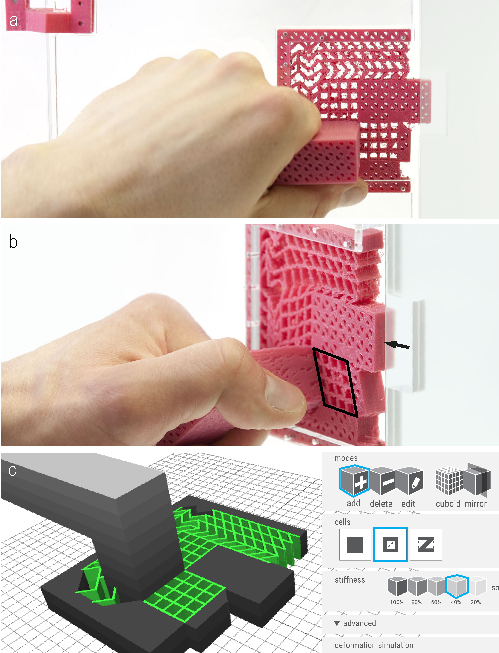
\includegraphics[width=\textwidth]{chapters/metamaterial-mechanisms-FIG/1-embedded-door-latch-figure1.pdf}
    \caption[Short figure name.]{(a) This door latch is implemented as a metamaterial mechanism; it consists of a single block of material based on a regular grid of cells that together implement handle, latch, and springs. (b) Turning the handle causes the central hinge array to deform and to pull the latch inwards, which unlocks the door. (c) We created this mechanism in our custom editor. Here, we placed two hinge arrays that mechanically couple the handle to the latch, and cells that couple to the doorframe.
    \label{fig:1 metanism-door latch}}
\end{figure}

While most of the object consists of \textit{rigid cells} (cells that are reinforced with a diagonal), the object also contains several rectangular regions of cells that lack such a diagonal reinforcement. These are the key to creating mechanisms, as they are able to deform in a very specific way: when subjected to an external force, these cells shear and thereby apply a force to their neighboring cells. We will discuss throughout the remainder of this paper how this basic principle allows creating mechanisms. 

Metamaterial mechanisms are simple. While the traditional door latch mechanism shown in Figure \ref{fig:2 metanism-traditional door latch} consists of several parts, including an axle, bearings, springs, etc., the metamaterial door latch in Figure \ref{fig:1 metanism-door latch} consists of a single block of material, as it is groups of cells inside the object that perform the mechanical function.

\begin{figure} [h]
    \includegraphics[width=\textwidth]{chapters/metamaterial-mechanisms-FIG/2-traditional-door-latch-labeled.pdf}
    \caption[Short figure name.]{This traditional door latch design consists of many parts, thus requires assembly. 
    \label{fig:2 metanism-traditional door latch}}
\end{figure}

While in previous work metamaterials were typically generated by scripts \cite{Mullin2007, Paulose2015}, creating mechanisms requires a dedicated design/engineering process that we argue is best performed by means of an interactive editor. Figure \ref{fig:1 metanism-door latch}c shows a preview of the custom 3D editor we created specifically to allow users to create and modify metamaterial mechanisms. It contains a range of functions that help users assemble specialized cells into basic mechanisms and to assemble such basic mechanisms into more complex mechanisms and simple machines. Using this editor, we have created a series of demo objects including the door latch from Figure \ref{fig:1 metanism-door latch}, a Jansen walker, or a functional pair of pliers. Our examples were printed on an \textit{Ultimaker 2} 3D printer using \textit{NinjaFlex} filament (in pink). The basic mechanisms (hinge, four-bar) were laser cut from $3\, \mathrm{mm}$ rubber foam (in black).


\section{Contribution, benefits, and limitations}

Our main contribution is the concept of metamaterial mechanisms. Our main software contribution is a specialized editor that allows users to create them.

We extend the research field of metamaterials by contributing a general-purpose approach to creating mechanisms. Mechanisms are a new genre of metamaterial structures that is of higher complexity and that exploits more degrees of freedom than previous work in this field, and that allow metamaterials to tackle problems they have traditionally not been able to address. 

Compared to traditional multi-part mechanisms, metamaterial mechanisms offer several benefits. (1) The resulting devices consist of a single part. They can thus be created using particularly simple fabrication processes, such as single-material 3D printers (e.g., FDM printers). (2) As they consist of a single piece, they require no assembly. (3) Since the movement is performed by deformation there is virtually no friction, no need for lubrication, and thus for maintenance \cite{Howell2013}.

However, the resulting designs are also subject to limitations. Adding more cells increases the stiffness, and as a result, metamaterial mechanisms are not suitable for mechanisms that are to be operated with very small forces. Furthermore, our approach is unable to produce continuous rotation. Objects such as the Jansen walker, for example, thus require a separate axle. Also, cell designs are limited by the quality of the 3D printer. In particular, shear cells work best if their internal hinges are thin, which requires high-resolution 3D printers. Finally, while our editor vastly simplifies the creation of metamaterial mechanisms, any type of mechanical engineering requires experience---and metamaterial mechanisms are no exception here.


\section{Members \& hinges based on cells}

The mechanism behind the door latch in Figure \ref{fig:1 metanism-door latch} ultimately consists of rigid regions (such as the latch itself), which we will refer to as members and compliant regions that implement hinges (such as the region right of the handle). Members and hinges both consist of cells on an evenly spaced grid. This is the general schema behind metamaterial mechanisms.

In this section, we take a closer look at these two basic elements and illustrate how to use them to build mechanisms. 


\subsection{Members from cells}

Members consist of rigid cells. A rigid unit cell is reinforced with a diagonal, as shown in Figure \ref{fig:3-basic-grid-structure}. The diagonal reinforces the cells against shear forces and thus makes them rigid. Adding two diagonals is possible, but not necessary, hence we use only one diagonal for our member structures in order to save material.

\begin{figure} [h]
    
\includegraphics[width=\textwidth]{chapters/metamaterial-mechanisms-FIG/3-basic-grid-structure.pdf}
    \caption[Short figure name.]{(a) The basic grid structure allows reinforcing rigid member cells (b-c) with one diagonal or (d) two diagonals.
    \label{fig:3-basic-grid-structure}}
\end{figure}

While we will focus our discussion on only two types of cells, namely stiff member cells and shearable hinge cells, our research can be combined with any other system of metamaterials already done as long as they are on a cube grid. Just to pick one example, we can make cells soft or hard \cite{Chu2008a} by weakening their beams so as to allow the cells to compress more easily, or reinforcing their beams to make the cells stiffer (Figure \ref{fig:4-cells-increasing-stiffness}). 

\begin{figure} [h]
    
\includegraphics[width=\textwidth]{chapters/metamaterial-mechanisms-FIG/4-cells-increasing-stiffness.pdf}
    \caption[Short figure name.]{Member cells of increasing stiffness.
    \label{fig:4-cells-increasing-stiffness}}
\end{figure}


\subsection{Hinges}

We can create a (naïve) hinge by connecting two cells diagonally as shown in Figure \ref{fig:5-hinge-array}a. Here the material connecting the two cell blocks forms a thin flexible hinge made from the same material as the two rigid members it connects. As common for this type of contraption, we will refer to it as a living hinge.

\begin{figure} [h]
    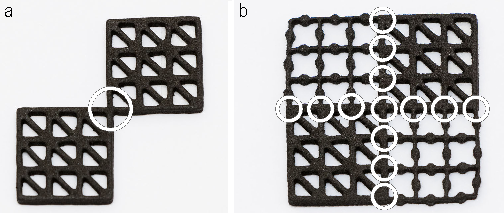
\includegraphics[width=\textwidth]{chapters/metamaterial-mechanisms-FIG/5-hinge-array.pdf}
    \caption[Short figure name.]{(a) A naïve living hinge, (b) reinforced with two arrays of hinges. To showcase the deformation, we laser cut these structures from rubber foam.
    \label{fig:5-hinge-array}}
\end{figure}

Next we add reinforcement to the hinge. Metamaterial cells can, at least in theory, be arbitrarily small—the hinge connecting two cells can thus arbitrarily thin, making mechanisms based on such naïve living hinges fragile, i.e., pulling them apart with very little force will rip them off.

We address the issue by extending the living hinge into an array of living hinges, as illustrated by Figure \ref{fig:5-hinge-array}b. We call them hinge arrays. Figure \ref{fig:6-simple-hinge-rotation} shows that the array flexes in concert with the main living hinge. The hinge array on the inside of the rotation complies by compressing in a shearing motion; the hinge array on the outside complies by stretching in a shearing motion. All hinges together perform a rotation around the original living hinge.

\begin{figure} [h]
    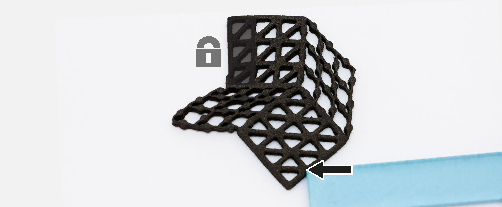
\includegraphics[width=\textwidth]{chapters/metamaterial-mechanisms-FIG/6-simple-hinge-rotation.pdf}
    \caption[Short figure name.]{The reinforced hinge in action. Note how the hinge array deforms as one while the rigid members remain undeformed. (Cells with gray tinted backgrounds are anchored to the ground, as indicated by the lock symbol. We are pushing in the direction of the arrow using the blue rod).
    \label{fig:6-simple-hinge-rotation}}
\end{figure}

However, when this reinforced hinge is stretched as shown in Figure \ref{fig:7-hinge-tear}a, its hinge arrays evade the tension by shearing. As a result, all tension rests on the central living hinge, causing it to break. As shown in Figure \ref{fig:7-hinge-tear}b, we address this by adding a border of rigid cells to the hinge arrays. These borders force all living hinges to follow the motion of the central living hinge, thereby support the main hinge by assuming part of the load, which distributes the tension across all the hinges.

Tensile strength increases linearly with the diagonal of the hinge array, because tension applies to the shortest path of hinges to tear in order to separate the two members. The tensile strength of the hinge array in Figure \ref{fig:7-hinge-tear}, for example, is $7\times$ larger than of a single hinge.

\begin{figure} [h]
    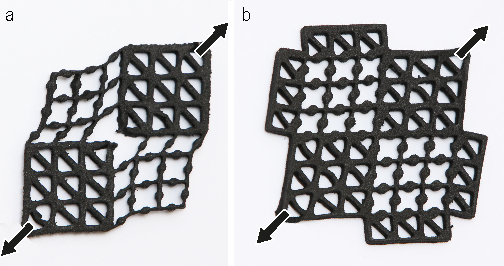
\includegraphics[width=\textwidth]{chapters/metamaterial-mechanisms-FIG/7-hinge-tear.pdf}
    \caption[Short figure name.]{(a) When this hinge array is stretched as shown, the central hinge breaks. (b) We address this by adding borders of rigid cells; they help distribute the tension more evenly. 
    \label{fig:7-hinge-tear}}
\end{figure}

Figure \ref{fig:8-simulation-tear-and-rotate} shows the resulting stress distribution after reinforcement (simulated using Autodesk Fusion 360; light colors indicate regions of high mechanical stress).

Hinge arrays also allow tuning the bending stiffness of a hinge, e.g., to make sure the door latch in Figure \ref{fig:1 metanism-door latch} offers appropriate resistance when pushed down, as well as sufficient force to push the handle back up. Bending stiffness increases proportional to the surface of the hinge array, i.e., $(width+1) \times (height+1)$, as all individual hinges need to be bent. The hinge array in Figure \ref{fig:7-hinge-tear}, for example, uses 2 hinge arrays of $(3+1) \times (3+1) = 32$ hinges, thus it takes 32 times more force to bend it than the single hinge in the center.

\begin{figure} [h]
    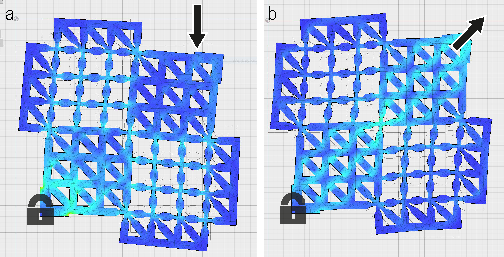
\includegraphics[width=\textwidth]{chapters/metamaterial-mechanisms-FIG/8-simulation-tear-and-rotate.pdf}
    \caption[Short figure name.]{Resulting stress distribution on (a) rotation and (b) tension after reinforcement.
    \label{fig:8-simulation-tear-and-rotate}}
\end{figure}


\subsection{Four-bars implement parallel motion}

In Figure \ref{fig:9-metamaterial-four-bar}, we use the concept of rigid members connected by hinge arrays to construct a shearing frame of four links, also known as \textit{four-bars}. Four-bars consist of four members attached to the \textit{opposite} sides of a hinge array (unlike the reinforced hinge, which consists of two members attached to \textit{adjacent} sides of a hinge array). It then contains the two opposing members to parallel motion. Note how the rigid member that is pushed to the left in Figure \ref{fig:9-metamaterial-four-bar}b rotates, while the top member moves in parallel with the rigid area underneath it.

\begin{figure} [h]
    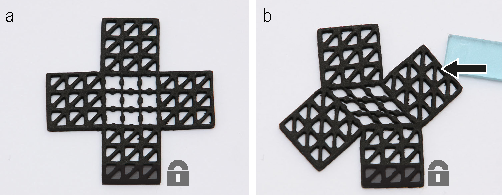
\includegraphics[width=\textwidth]{chapters/metamaterial-mechanisms-FIG/9-metamaterial-four-bar.pdf}
    \caption[Short figure name.]{A metamaterial four-bar. 
    \label{fig:9-metamaterial-four-bar}}
\end{figure}

In Figure \ref{fig:10-pliers-ninjaflex} we exploit this property of the four-bar in order to create a functional pair of pliers. The hinge array in the center acts as a four-bar that connects the right handle with the left bracket \textit{and} the left handle with the right bracket, yet allows the two sides to move with respect to each other---somewhat similar to how the axle in a traditional pair of scissors allows the two handle and blade elements to move with respect to each other.

\begin{figure} [h]
    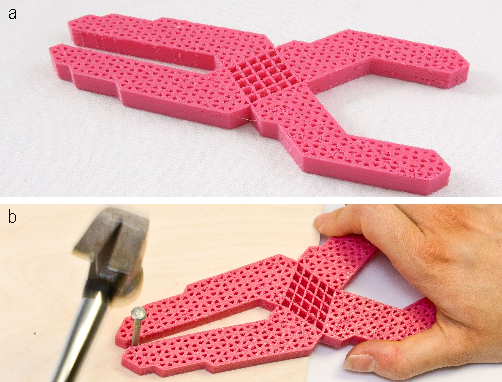
\includegraphics[width=\textwidth]{chapters/metamaterial-mechanisms-FIG/10-pliers-ninjaflex.pdf}
    \caption[Short figure name.]{(a) This pair of pliers is based on a single metamaterial four-bar. (b) When the user applies a force to the handles, the hinge array in the center transmits this force to the brackets, and the pliers close. 
    \label{fig:10-pliers-ninjaflex}}
\end{figure}


\subsection{Cascades of hinge arrays}

We chain multiple four-bars to create a scissors mechanism, which is a linkage that arranges links in a criss-cross pattern and is used. Figure \ref{fig:11-pantograph} shows how we implement a pantograph by chaining multiple metamaterial four-bars. The pantograph holds two pencils. While one pencil is moved by the user to draw, the second pencil moves along and replicates the user’s drawing.
 
\begin{figure} [h]  
    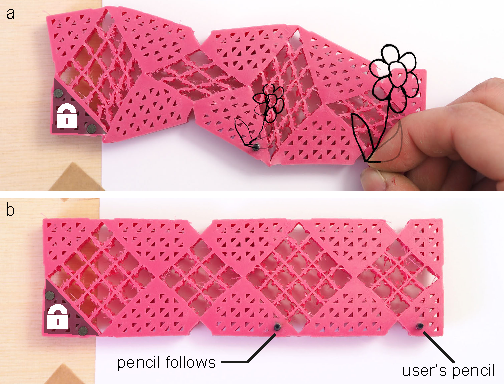
\includegraphics[width=\textwidth]{chapters/metamaterial-mechanisms-FIG/11-pantograph.pdf}
    \caption[Short figure name.]{The user draws a flower using (a) our metamaterial pantograph, which (b) replicates the flower as the user is drawing. 
    \label{fig:11-pantograph}}
\end{figure}


\section{The key: The shear cell}
\label{section:shear-cell}

So far, we only introduced the rigid cell. However, without explicitly mentioning it, the previous section introduced a second type of cell: a cell designed to shear. Unlike the rigid cell, this \textit{shear cell} is designed to deform when a force is applied, more specifically to \textit{shear} (Figure \ref{fig:12-shear-cell-deformation}). 

\begin{figure} [h]  
    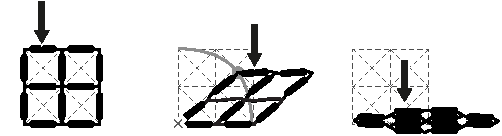
\includegraphics[width=\textwidth]{chapters/metamaterial-mechanisms-FIG/12-shear-cell-deformation.pdf}
    \caption[Short figure name.]{When a shear cell in this $2 \times 2$ block is subject to compression forces, it complies by shearing on a circular trajectory until its members are packed tightly.
    \label{fig:12-shear-cell-deformation}}
\end{figure}

As illustrated by Figure \ref{fig:12-shear-cell-deformation}, shear cells compress when a force is applied. The cell itself consists of miniature members and miniature living hinges---similar to the macroscopic structures we build from them. When a force is applied, the hinges start to bend, while the members largely maintain their shape (increasing the thickness of a beam results in a cubed increase in stiffness). The shear cell resists the external force based on the springiness of its hinges, until eventually the members touch and the resulting tightly packed block of cells is not compressible anymore apart from the compressibility of the material itself.

Since shear cells are based on an unit cell of our grid, they are always oriented along the cardinal directions. To allow handling forces and shearing along additional orientations, we introduce rotated hinges. As illustrated by Figure \ref{fig:13-diamond-cell-deformation}, we obtain a rotated design by combining groups of $2 \times 2$ cells, each of which contains (only) a diagonal. 

\begin{figure} [h]  
    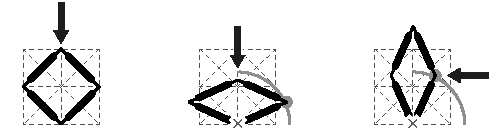
\includegraphics[width=\textwidth]{chapters/metamaterial-mechanisms-FIG/13-diamond-cell-deformation.pdf}
    \caption[Short figure name.]{The rotated shear cell.
    \label{fig:13-diamond-cell-deformation}}
\end{figure}

Combining regular and rotated hinges allows us to engineer additional mechanisms, such as the leg pair of a Jansen walker mechanism that is shown in Figure \ref{fig:14-jansen-walker}. Each leg consists of 6 hinges that make up the organic walking motion when the center is actuated on a circular path using a crank. One hinge per leg, however, needs to be constrained so as to only rotate, not translate. We implement this by adding a layer of two metamaterial hinges for the two legs that are connected to stay at constant distance but decoupled to move independently from each other. 

\begin{figure} [!h]
    \centering
    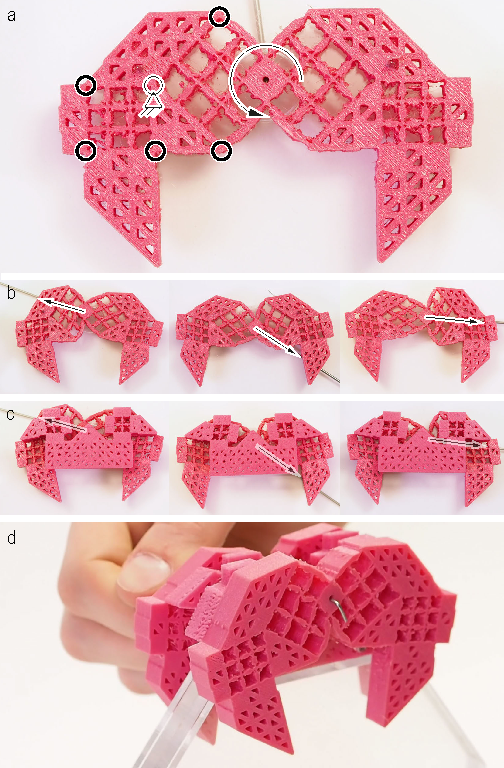
\includegraphics[width=0.83\textwidth]{chapters/metamaterial-mechanisms-FIG/14-jansen-walker.pdf}
    \caption[Short figure name.]{(a) Each leg of the Jansen walker has 6 hinges. (b) As the center is actuated by a crank, the legs deform in a walking motion. (c) We constrain two hinges to rotate, but not translate, using a layer of hinges. (d) The complete walker.
    \label{fig:14-jansen-walker}}
\end{figure}

Finally, we have created a third type of shear cell by leaving out one of the Cartesian members. It is shown in Figure \ref{fig:15-z-cell-deformation} and we refer to it as \textit{z-cell.}

\begin{figure} [!h]  
    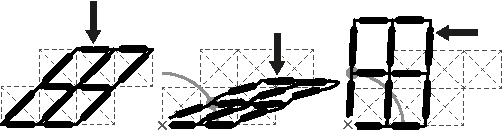
\includegraphics[width=\textwidth]{chapters/metamaterial-mechanisms-FIG/15-z-cell-deformation.pdf}
    \caption[Short figure name.]{"z-cells" shear on a larger circular path than regular shear cells, which is also rotated by 45°. 
    \label{fig:15-z-cell-deformation}}
\end{figure}

Z-cells are very similar to regular shear cells, except that they are “pre-sheared”, which results in three differences: (1) they have an asymmetric shearing behavior (range of 135° vs. 45°), (2) they expand as they shear against their pre-sheared direction, and (3) compress in the other direction.

Figure \ref{fig:16-switch} shows a switch based on z-cells. The button stays parallel while going down to hit the contact point reliably. A similar switch implemented from only soft and hard cells requires making very thin beams to allow the switch to deform. However, this does not implement a well-defined directional movement and closing at the contact point is not ensured.

\begin{figure} [h]
    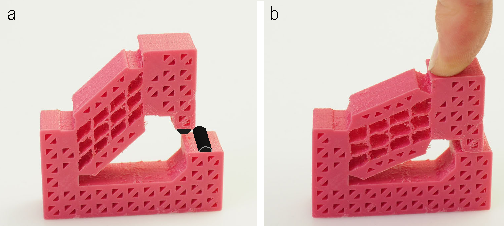
\includegraphics[width=\textwidth]{chapters/metamaterial-mechanisms-FIG/16-switch.pdf}
    \caption[Short figure name.]{(a) This switch is designed based on z-cells, which allow it to compress in a controlled motion and (b) close reliably at the black contact point. 
    \label{fig:16-switch}}
\end{figure}


\subsection{Padding}

Metamaterial mechanisms enable directional movement of regions of material, i.e., they occupy space when they are in their deformed state that was not occupied in their undeformed state. Most of our examples---the pliers, the walker, or the pantograph---are self-contained and can deform independently. However, the door latch is not self-contained but embedded in a rigid door. This requires appropriate clearance for the respective region to move into. 

We surround the door latch shown in Figure \ref{fig:17-padding-movement} with what we call padding areas. Padding areas consist of cells that are not intended to transmit any forces, but rather to receive the forces exerted by the main mechanism. The padding serves two purposes here: (1) to connect the movable door latch with the rigid door and (2) to increase its stability, i.e., to prevent the mechanism from buckling out of plane and add support against operation in unintended directions. In case the handle is pushed up, the z-cells above the latch prevent the latch from moving outward (to the right).

\begin{figure} [!h]
    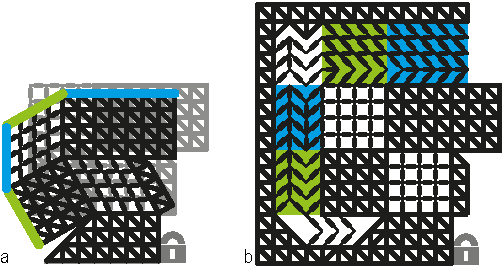
\includegraphics[width=\textwidth]{chapters/metamaterial-mechanisms-FIG/17-padding-movement.pdf}
    \caption[Short figure name.]{(a) When the door latch deforms, the edges labeled in blue remain parallel, while the green edges rotate. (b) Consequently, we reinforce the green regions using padding cells that allow for translation and rotation deformation, while we reinforce the blue regions to only allow for translation. 
    \label{fig:17-padding-movement}}
\end{figure}

Figure \ref{fig:17-padding-movement}a shows that after the door latch mechanism is deformed we see two types of transformations on the outside edges: (1) a parallel movement that is indicated by the blue line and (2) a rotational movement of the edge indicated by the green line. Additionally, all the edges undergo a vertical and horizontal translation. For all outside edges we need to allow translation and for some we need to additionally allow rotation. Therefore, the latch mechanism in Figure \ref{fig:17-padding-movement}b uses two types of padding cells, chosen to allow for the intended movement, yet to suppress other types of movement.

\paragraph{Z-cell padding absorbs parallel movement,} like the movement of the latch. Z-cell padding allows a member on one side to translate in 2D with respect to a member on the other side and keeps the two members parallel. Since z-cells shear on a circular path that is rotated by 45°, they allow for a vertical extension of $\sqrt{2}-1$ cells and a horizontal displacement of 1 cell. We simply stack enough layers of z-cells to compensate for the downward and inward movement of the latch.

Note that we added one row of z-cells that is flipped. Figure \ref{fig:18-padding-trajectories}a shows that this additional row is necessary since the shear cells underneath the latch and the z-cells above the latch travel on opposing circular trajectories and cannot pass each other. The flipped row of z-cells however moves upwards (Figure \ref{fig:18-padding-trajectories}b) and gives space for the lower row of z-cells to pass and thus the latch to move.

\begin{figure} [h]  
    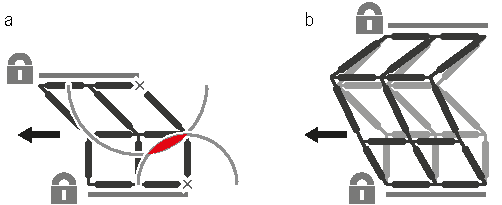
\includegraphics[width=\textwidth]{chapters/metamaterial-mechanisms-FIG/18-padding-trajectories.pdf}
    \caption[Short figure name.]{(a) The shear cells cannot pass each other (red area), (b) therefore we add a flipped row of z-cells that compress and give space for the other shearing cells to move.
    \label{fig:18-padding-trajectories}}
\end{figure}

\paragraph{V-cell padding absorbs rotation.} V-cells are similar to the flipped z-cell group, but they additionally allow two opposing members to rotate, as shown in Figure \ref{fig:19-v-cells}. We add this degree of freedom by removing the vertical beam from the z-cells. We use v-cells in combination with z-cells on the rotating edges illustrated by Figure \ref{fig:17-padding-movement}b. 

\begin{figure} [h]  
    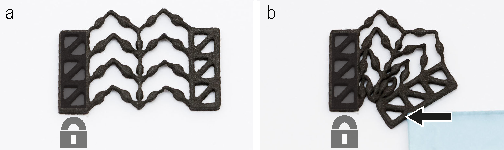
\includegraphics[width=\textwidth]{chapters/metamaterial-mechanisms-FIG/19-v-cells.pdf}
    \caption[Short figure name.]{V-cells allow for rotation, as well as for compression and extension.
    \label{fig:19-v-cells}}
\end{figure}


\section{Hierarchy of metamaterial mechanisms}

In this section, we presented the main elements of metamaterial mechanisms. These elements form the following five-level hierarchy.

\begin{enumerate}
    \item \textit{Cells} are the lowest-level element of metamaterial mechanisms and perform an elementary mechanical function. We presented shear cells, which implement four-bars on a cell level, as well as z-cells.
    \item \textit{Compound cells} still perform an elementary function, yet are implemented using multiple physical cells, such as the rotated shear cell or the v-cell.
    \item \textit{Basic mechanisms} are created by repeating cells, in particular the reinforced hinge mechanism and the four-bar mechanism.
    \item \textit{Compound mechanisms} consist of multiple basic mechanisms, such as the scissors mechanism implemented in the pantograph.
    \item \textit{Machines} perform a mechanical function and consist of one or more basic or compound mechanisms, such as the door latch (Figure \ref{fig:1 metanism-door latch} and Figure \ref{fig:17-padding-movement}), the pliers (Figure \ref{fig:10-pliers-ninjaflex}), the Jansen walker (Figure \ref{fig:14-jansen-walker}).
    
\end{enumerate}


% \section{Metamaterial Mechanisms Editor}

% To allow users to design, fabricate, and test metamaterials containing mechanisms we implemented the specialized editor shown in Figure \ref{fig:20-editor-ui}. 

% \begin{figure} [h]  
%     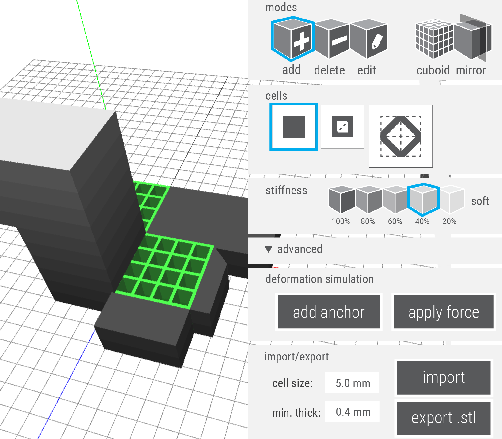
\includegraphics[width=\textwidth]{chapters/metamaterial-mechanisms-FIG/20-editor-ui.pdf}
%     \caption[Short figure name.]{Our editor allows users to edit and simulate the deformation of metamaterial mechanisms interactively. 
%     \label{fig:20-editor-ui}}
% \end{figure}

% The main intent behind it is not only to make the editing process more efficient than the more traditional script-based editing, but also to provide users with an overview of their design, encouraging design by trial-and-error. 

% Our editor is based on interaction techniques known from voxel editors (such as \textcolor{cyan}{[35]}). However, in addition our software also offers specific supports for creating mechanisms, such as tools for drawing hinge arrays, etc. In order to allow users to validate their designs, the editor also allows them to apply forces and see how the object deforms in order to then refine their design directly inside the editor, before exporting to the 3D printer.


% \subsection{Walkthrough}

% Figure \ref{fig:21-editor-walkthrough} illustrates how we created the door handle.

% (a) We start by creating a block of rigid cells using the \textit{add brush} (we can remove cells using the \textit{delete brush}). Here we use the tool in \textit{cuboid mode}, which allows us to draw a filled rectangular region at once by just drawing the diagonal. (b) By adding another two cuboids on top, we create the handle.

% (c) We select the \textit{shear brush}. Still in cuboid mode, we paint the central hinge array using a single drag interaction, which causes rigid cells to turn into shear cells. Even though the block of material we painted on is two cells high, the shear brush paints cells all the way through---as we can tell from the sidewall now being all green. This is one of the features of this brush: since shear cells backed by rigid cells would still be rigid, thus have no effect, the shear brush always cuts shear cells through the entire object. 

% \begin{figure} [h]  
%     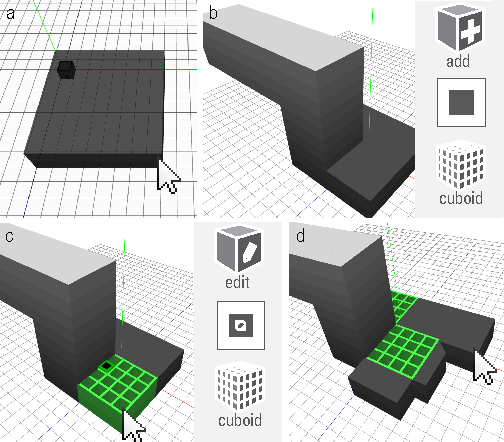
\includegraphics[width=\textwidth]{chapters/metamaterial-mechanisms-FIG/21-editor-walkthrough.pdf}
%     \caption[Short figure name.]{Walkthrough of the creating door latch mechanism. The UI elements on the right show the active tools for the respective interaction steps.
%     \label{fig:21-editor-walkthrough}}
% \end{figure}

% We now verify our design directly from within the editor, as illustrated by Figure \ref{fig:22-simulation-walkthrough}. (a) We select the anchor tool and use it to place a few anchor points at the bottom, indicating that the door latch is here rigidly connected to the doorframe. (b) Now we use the force tool to apply a force to the door handle. We attach a force arrow to one of the handle’s cell vertices. As we are building up the force by dragging the force tool the system already responds by showing the resulting deformation of our door latch. 

% \begin{figure} [h]  
%     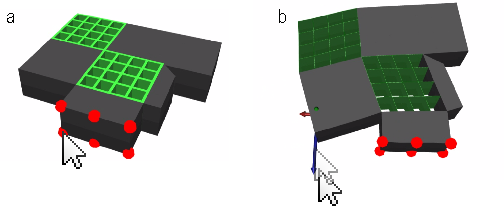
\includegraphics[width=\textwidth]{chapters/metamaterial-mechanisms-FIG/22-simulation-walkthrough.pdf}
%     \caption[Short figure name.]{To simulate the deformation in real-time in the editor, (a) users set anchor points and (b) adjust forces using the force tool. 
%     \label{fig:22-simulation-walkthrough}}
% \end{figure}


% \subsection{Multiple dimensions}

% While the door latch mechanism actuates in only two dimensions, our editor also supports placing mechanisms in 3 dimensions. The latch mechanism shown in Figure \ref{fig:23-3D-object}, for example, combines a horizontal hinge array (blue) and a vertical hinge array (green) in order to create a mechanism that users operate by pressing down, sliding over, and releasing. 

% Our editor color-codes mechanisms automatically according to their orientation in space. This is intended to provide users with a fast overview of the main dimensions of action in their devices and to help recognize hinge arrays from odd viewing angles. In the latch example, green denotes ``shearing on the x/z plane" and blue stands for ``shearing on the x/y plane". Analogously, red stands for ``shearing on the y/z plane".

% \begin{figure} [h]  
%     \includegraphics[width=\textwidth]{chapters/metamaterial-mechanisms-FIG/23-3D-object.pdf}
%     \caption[Short figure name.]{This latch requires the ability to shear on two planes, i.e., on the x/z plane denoted in green, and on the on x/y plane indicated in blue.
%     \label{fig:23-3D-object}}
% \end{figure}

% Note that hinge arrays can overlap. In this case, cells at the intersection bear the combination of all holes. These cells are rendered as the additive mixture of the involved colors, such as yellow, for cells at the intersection between green and red.


% \subsection{Integration with other metamaterial systems}

% The shear cell is the main element that enables metamaterial mechanisms. However, to allow for the integration with metamaterials by other researchers, the editor can be extended to allow for other cell types. 

% In order to allow users to explore their own cell types, we offer the advanced panel shown in Figure \ref{fig:24-advanced-cell-builder}. Users compose cells from individual edges by selecting the respective edges. The editor automatically adds all custom cells used in the current model to the cells panel for quick reuse. 

% \begin{figure} [h]  
%     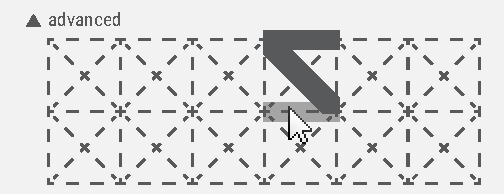
\includegraphics[width=\textwidth]{chapters/metamaterial-mechanisms-FIG/24-advanced-cell-builder.pdf}
%     \caption[Short figure name.]{Users compose custom cells by adding individual edges in the ``advanced" panel.
%     \label{fig:24-advanced-cell-builder}}
% \end{figure}

% Furthermore, users can also create and store groups of cells, for example to create auxetic materials \textcolor{cyan}{[6, 18]}, as shown in Figure \ref{fig:25-advanced-cell-groups}. Since metamaterial mechanisms adhere to the standard structure of 3D cell grids that is common for metamaterials, they integrate with earlier research \textcolor{cyan}{[24, 30]}.

% \begin{figure} [h]  
%     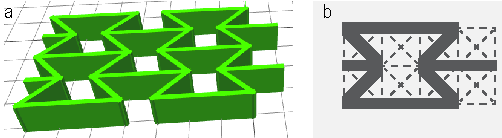
\includegraphics[width=\textwidth]{chapters/metamaterial-mechanisms-FIG/25-advanced-cell-groups.pdf}
%     \caption[Short figure name.]{Users add groups of cells, here they create an auxetic material from a $4 \times 2$ group of cells.
%     \label{fig:25-advanced-cell-groups}}
% \end{figure}


% \section{System Implementation}
% \label{section:mechanisms-editor}

% In the following, we provide details on the internal processes implemented in our metamaterial mechanisms editor.

% \subsection{Import}

% Users can import mesh geometries directly into our editor. We voxelize the meshes using \textit{binvox}\footnote{\url{http://www.cs.princeton.edu/~min/binvox/}}  according to the cell size that the user defined. 

% \subsection{Editor}
% Our 3D editor is based on WebGL and uses three.js. Internally, the editor creates a dictionary of cells that can be accessed using their position on the grid. Each cell is defined by the 8 vertices making up its bounding box by and the edges that define how the vertices are connected. Note that not all 8 vertices need to be connected by edges. 

% All vertices lie on our uniform 3-dimensional grid. To generate the 3D cells' structures, i.e., to generate 3D beams from 1D edges, we apply an offset to the vertices’ positions on the GPU. Since WebGL does not offer geometry shaders, we use a vertex shader and pass the offset direction and the cell’s position with each vertex. The 8 vertices that form a beam are offset uniformly from the two edge vertices on the GPU. To pass additional information about the color and thickness of beams to the shader, we generate a texture where each pixel holds these data for one cell. The color maps directly and the thickness is encoded in the alpha component. In the shader, every vertex looks up its thickness in the texture and calculates the offsets for the new vertices that render a beam from an edge. This enables us to emulate a geometry shader in WebGL and perform all geometry processing on the GPU, which keeps the user experience of our editor smooth.

% \subsection{Simulation}
% For simulating the deformation of the user’s cell structure, we use the finite elements solver \textit{karamba}\footnote{\url{http://www.karamba3d.com/}}, which is a plugin-for Grasshopper/Rhinoceros. We implemented a custom C\#-Grasshopper-component that receives the mesh data (vertices and edges) and the data for the simulation (anchored vertices, force and vertex where the force applies) via a web socket connection. When the simulation is complete, a second custom component receives the transformed mesh vertices and sends them back to the editor. The vertices are kept in the same order within the array as they were received from the editor. We run the simulation on a separate machine to keep the editor running smoothly. 

% Maintaining the order of the vertices is important to enable geometry processing on the GPU. In the editor, we generate another texture and store the transformed vertices, where XYZ is mapped to RGB. The shader knows the vertex' undeformed position on the grid and looks up the deformed position in the texture.

% Depending on the size of the object that is simulated, solving for the deformation can lead to perceivable delays. To compensate for this, our editor interpolates the deformation while the response from the simulation is pending. To do so, we pass the last force where we received the transformation from the server, and the current force that was submitted to the simulation and interpolate the vertex transformation linearly.

% \subsection{Export}

% We generate an .stl file for the user that is ready to be 3D printed. Our export is based on OpenJSCAD. In this step, we refine the cell structure from the simplified editor view to our beams with stiff members and thin living hinges. For every edge that belongs to a shear cell, we create a beam with a thick part in the middle. Edges that are part of rigid cells are generated as simple straight beams. Finally, we use OpenJSCAD's built-in render engine, which we invoke directly from our 3D editor to perform the union operations and generate the .stl file.


\section{Editing metamaterial mechanisms}

To allow users to design, fabricate, and test metamaterials containing mechanisms we implemented the specialized editor shown in Figure \ref{fig:20-editor-ui}. 

\begin{figure} [h]
    \centering
    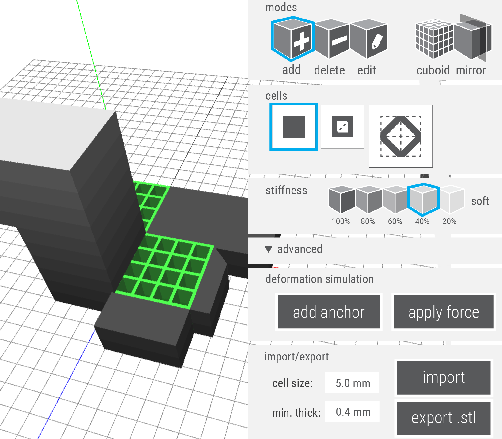
\includegraphics[width=0.9\textwidth]{chapters/metamaterial-mechanisms-FIG/20-editor-ui.pdf}
    \caption[Short figure name.]{Our editor allows users to edit and simulate the deformation of metamaterial mechanisms interactively. 
    \label{fig:20-editor-ui}}
\end{figure}

The main intent behind it is not only to make the editing process more efficient than the more traditional script-based editing, but also to provide users with an overview of their design, encouraging design by trial-and-error. 

Our editor is based on interaction techniques known from voxel editors (such  as \cite{VoxCAD2018}). However, in addition our software also offers specific supports for creating mechanisms, such as tools for drawing hinge arrays, etc. In order to allow users to validate their designs, the editor also allows them to apply forces and see how the object deforms in order to then refine their design directly inside the editor, before exporting to the 3D printer.

%\section{Encapsulating domain knowledge into the editor}

\subsection{User interaction}

Figure \ref{fig:21-editor-walkthrough} illustrates how users create the door handle example.

\begin{figure} [h]
    \centering
    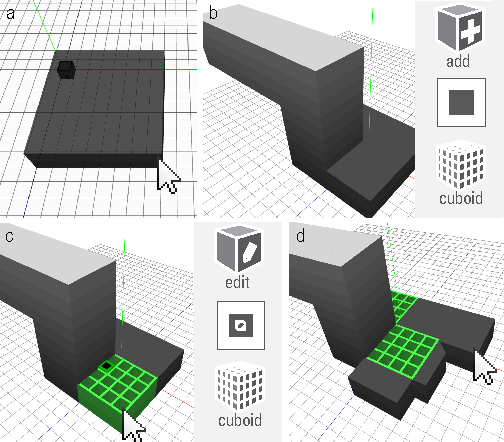
\includegraphics[width=0.85\textwidth]{chapters/metamaterial-mechanisms-FIG/21-editor-walkthrough.pdf}
    \caption[Short figure name.]{Walkthrough of the creating door latch mechanism. The UI elements on the right show the active tools for the respective interaction steps.
    \label{fig:21-editor-walkthrough}}
\end{figure}

(a) Users start by creating a block of rigid cells using the \textit{add brush}. They can remove cells using the \textit{delete brush}. Here, users utilize the tool in \textit{cuboid mode}, which allows them to draw a filled rectangular region at once by just drawing the diagonal. (b) By adding another two cuboids on top, users create the handle.

(c) Next, Users select the \textit{shear brush}. Still in cuboid mode, they paint the central hinge array using a single drag interaction, which causes rigid cells to turn into shear cells. Even though the block of material that users painted on is two cells high, the shear brush paints cells all the way through---as they can tell from the sidewall now being all green. This is one of the features of this brush: since shear cells backed by rigid cells would still be rigid, thus have no effect, the shear brush always cuts shear cells through the entire object. 


\subsection{Simulating deformation}
Users now verify their design directly from within the editor, as illustrated by Figure \ref{fig:22-simulation-walkthrough}. 

\begin{figure} [h]
    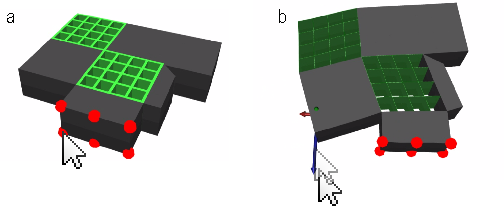
\includegraphics[width=\textwidth]{chapters/metamaterial-mechanisms-FIG/22-simulation-walkthrough.pdf}
    \caption[Short figure name.]{To simulate the deformation in real-time in the editor, (a) users set anchor points and (b) adjust forces using the force tool. 
    \label{fig:22-simulation-walkthrough}}
\end{figure}

(a) They select the anchor tool and use it to place a few anchor points at the bottom, indicating that the door latch is rigidly connected to the doorframe there. (b) Now, they use the force tool to apply a force to the door handle. Users attach a force arrow to one of the handle’s cell vertices. As users are building up the force by dragging the force tool the system already responds by showing the resulting deformation of our door latch. 

\subsection{Multiple dimensions}
While the door latch mechanism actuates in only two dimensions, our editor also supports placing mechanisms in 3 dimensions. The latch mechanism shown in Figure \ref{fig:23-3D-object}, for example, combines a horizontal hinge array (blue) and a vertical hinge array (green) in order to create a mechanism that users operate by pressing down, sliding over, and releasing. 

\begin{figure} [h]
    \includegraphics[width=\textwidth]{chapters/metamaterial-mechanisms-FIG/23-3D-object.pdf}
    \caption[Short figure name.]{This latch requires the ability to shear on two planes, i.e., on the x/z plane denoted in green, and on the on x/y plane indicated in blue.
    \label{fig:23-3D-object}}
\end{figure}

Our editor color-codes mechanisms automatically according to their orientation in space. This is intended to provide users with a fast overview of the main dimensions of action in their devices and to help recognize hinge arrays from odd viewing angles. In the latch example, green denotes ``shearing on the x/z plane" and blue stands for ``shearing on the x/y plane". Analogously, red stands for ``shearing on the y/z plane".

Note that hinge arrays can overlap. In this case, cells at the intersection bear the combination of all holes. These cells are rendered as the additive mixture of the involved colors, such as yellow, for cells at the intersection between green and red.


\subsection{Integrating other metamaterial systems}

The shear cell is the main element that enables metamaterial mechanisms. However, to allow for the integration with metamaterials by other researchers, the editor can be extended to allow for other cell types. 

In order to allow users to explore their own cell types, we offer the advanced panel shown in Figure \ref{fig:24-advanced-cell-builder}. Users compose cells from individual edges by selecting the respective edges. The editor automatically adds all custom cells used in the current model to the cells panel for quick reuse. 

\begin{figure} [h]
    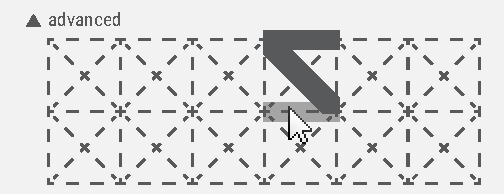
\includegraphics[width=\textwidth]{chapters/metamaterial-mechanisms-FIG/24-advanced-cell-builder.pdf}
    \caption[Short figure name.]{Users compose custom cells by adding individual edges in the ``advanced" panel.
    \label{fig:24-advanced-cell-builder}}
\end{figure}

Furthermore, users can also create and store groups of cells, for example to create auxetic materials \cite{Saxena2016}, as shown in Figure \ref{fig:25-advanced-cell-groups}. Since metamaterial mechanisms adhere to the standard structure of 3D cell grids that is common for metamaterials, they integrate with earlier research \cite{Panetta2015, Schumacher2015}.

\begin{figure} [h]
    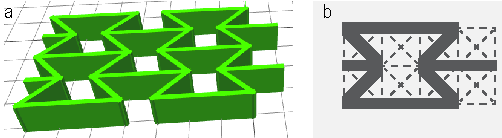
\includegraphics[width=\textwidth]{chapters/metamaterial-mechanisms-FIG/25-advanced-cell-groups.pdf}
    \caption[Short figure name.]{Users add groups of cells, here they create an auxetic material from a $4 \times 2$ group of cells.
    \label{fig:25-advanced-cell-groups}}
\end{figure}


\subsection{Implementation}
\label{section:mechanisms-editor}

In the following, we provide details on the internal processes implemented in our metamaterial mechanisms editor.

\subsubsection{Editor (.js)}
Our 3D editor is based on WebGL and uses three.js. Internally, the editor creates a dictionary of cells that can be accessed using their position on the grid. Each cell is defined by the 8 vertices making up its bounding box by and the edges that define how the vertices are connected. Note that not all 8 vertices need to be connected by edges. 

All vertices lie on our uniform 3-dimensional grid. To generate the 3D cells' structures, i.e., to generate 3D beams from 1D edges, we apply an offset to the vertices’ positions on the GPU. Since WebGL does not offer geometry shaders, we use a vertex shader and pass the offset direction and the cell’s position with each vertex. The 8 vertices that form a beam are offset uniformly from the two edge vertices on the GPU. To pass additional information about the color and thickness of beams to the shader, we generate a texture where each pixel holds these data for one cell. The color maps directly and the thickness is encoded in the alpha component. In the shader, every vertex looks up its thickness in the texture and calculates the offsets for the new vertices that render a beam from an edge. This enables us to emulate a geometry shader in WebGL and perform all geometry processing on the GPU, which keeps the user experience of our editor smooth.

\subsubsection{Simulation (C\#)}
For simulating the deformation of the user’s cell structure, we use the finite elements solver \textit{karamba}\footnote{\url{http://www.karamba3d.com/}} \cite{Preisinger2013}, which is a plugin-for Grasshopper/Rhinoceros. We implemented a custom C\#-Grasshopper-component that receives the mesh data (vertices and edges) and the data for the simulation (anchored vertices, force and vertex where the force applies) via a web socket connection. When the simulation is complete, a second custom component receives the transformed mesh vertices and sends them back to the editor. The vertices are kept in the same order within the array as they were received from the editor. We run the simulation on a separate machine to keep the editor running smoothly. 

Maintaining the order of the vertices is important to enable geometry processing on the GPU. In the editor, we generate another texture and store the transformed vertices, where XYZ is mapped to RGB. The shader knows the vertex' undeformed position on the grid and looks up the deformed position in the texture.

Depending on the size of the object that is simulated, solving for the deformation can lead to perceivable delays. To compensate for this, our editor interpolates the deformation while the response from the simulation is pending. To do so, we pass the last force where we received the transformation from the server, and the current force that was submitted to the simulation and interpolate the vertex transformation linearly.

\subsubsection{Import \& export}

Users can import mesh geometries directly into our editor. We load .stl meshes using the package 'stl-reader'\footnote{\url{https://www.npmjs.com/package/stl-reader}} and voxelize\footnote{\url{https://www.npmjs.com/package/voxelize}} them according to the cell size that the user defined. Once users are satisfied with their metamaterial, they can export their design as a 3D-printable .stl file. We use a constructive solid geometry (CSG) package\footnote{\url{https://www.npmjs.com/package/openjscad-csg}},
which we invoke directly from our 3D editor to perform the union operations and generate a triangulated .stl file.


\subsection{Software architecture}

We designed out software to be loosely coupled. As depicted in Figure \ref{fig:simple-software-architecture}, our editor communicates with the finite element analysis (FEA) tool via a web socket connection. This architecture allow the resource-intensive FEA calculations to be outsourced to a different computer (server) and to exchange the FEA component easily. 

\begin{figure} [h]
    \centering 
    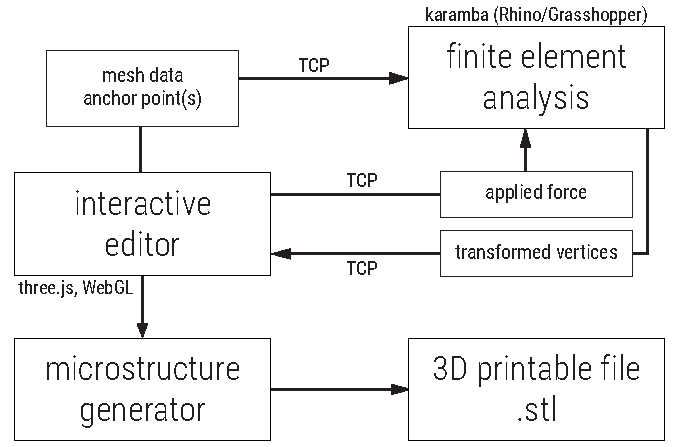
\includegraphics[width=0.85\textwidth]{chapters/software-FIG/simple-software-architecture.pdf}
    \caption[Short figure name.]{The software architecture or our metamaterial mechanism editor.
    \label{fig:simple-software-architecture}}
\end{figure}



\section{Discussion on material \& durability}

The ideal material for metamaterial mechanisms is (1) very elastic, i.e., goes back to its original shape without deforming permanently and (2) can withstand high forces without breaking. Spring steel fulfills these criteria well, yet is not possible to fabricate using today’s 3D printers. Among commonly available 3D printing materials, flexible materials (such as the TPU \textit{NinjaFlex} and \textit{SemiFlex}) fulfill these criteria well, more so than PLA and certain types of photo-curing resins (such as the \textit{spot-e} resin).

When we created 2D metamaterial mechanisms using our laser cutter, we obtained best results with rubber foam, more so than with ABS sheets and acrylic, which were not compliant enough. Our metamaterial mechanisms worked across fabrication techniques, since the functionality is determined by the cell structure. 

In our experience, material fatigue is not a problem, because we operate our metamaterial mechanisms, i.e., bend their living hinges, only to the point where they still fully return to their original shape (the material stays ``in the elastic region"). As an example, operating the NinjaFlex-printed Jansen walker shown in Figure \ref{fig:26-durability-test-jansen} about {\textasciitilde}5000 times (at {\textasciitilde}120 rpm) using a 300 W power drill, did not lead to any visible fatigue or damage in the metamaterial structure. 

\begin{figure} [h]  
    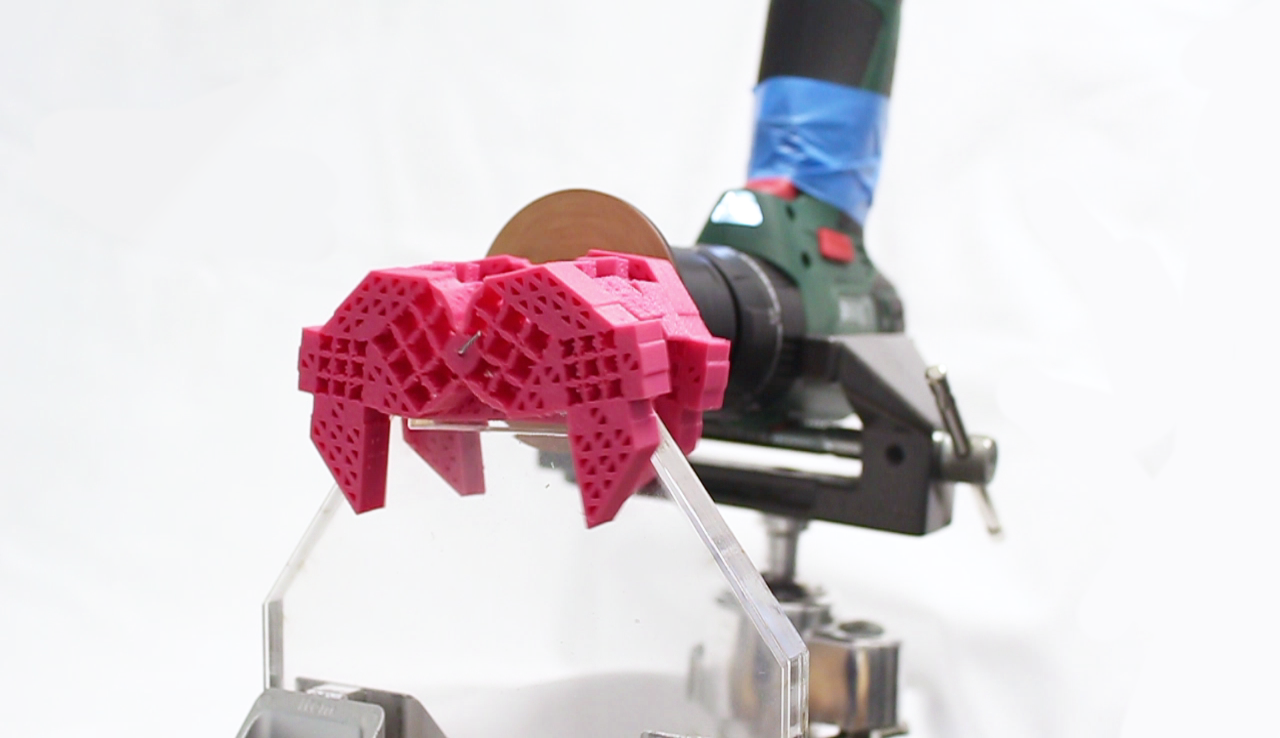
\includegraphics[width=\textwidth]{chapters/metamaterial-mechanisms-FIG/26-durability-test-jansen.png}
    \caption[Short figure name.]{We verified the durability of the Jansen walker by operating it {\textasciitilde}5000 times using a power drill.
    \label{fig:26-durability-test-jansen}}
\end{figure}

\section{Conclusions}
In this paper, we introduced metamaterial mechanisms. While metamaterials so far had been understood as materials, the main contribution of this paper is that we think of them as \textit{machines.}

On the most basic level, it was the shear cell that allowed us to implement this new perspective on metamaterials. The shear cell allowed us to redirect forces and thus to create basic mechanisms, compound mechanisms, and ultimately simple machines.

While our approach offers tangible benefits for users (e.g., it solves mechanical problems in a single part, thereby eliminates the need for assembly), we see the main promise of this work in that it allows us to achieve a deeper integration between the structural and the mechanical functions of materials.

% For future work, we plan to continue on this path by investigating how to integrate logical functions into material.

% Acknowledgements
% We thank David Lindlbauer for his insights and for printing many of our prototypes. We also thank Louis Kirsch, Moritz Hilscher, David Stangl, Arthur Silber, Friedrich Horschig and Noel Danz for their contribution to earlier versions of this work. 

\chapter{Understanding Metamaterial Mechanisms}
\label{chapter:Understanding-metamaterial-mechanisms}

% The recent rise of widely accessible fabrication machines, such as 3D printers or laser cutters, generated interest in non-experts to create and design their own devices. Their strive towards a future of personal- rather than mass-fabrication is supported by HCI researchers [4], who investigate techniques to directly interact with the machine [29][32][50], use real-world objects for content creation [48][49] or embed mechanisms [52] and electronics [38]. These works were mainly concerned with creating the outside shape of 3D objects.

% 3D printing technology, however, is unique in that it allows users to freely arrange matter in space. Researchers used this property to generate internal structures that, e.g., optimize the strength-to-weight ratio of 3D objects [25], allow arbitrarily shaped objects to spin [3], or to float in pre-defined poses [34].

% Pushing this idea further, researchers engineer microstructures that deform in a desired way. These structures are usually arranged on a regular grid and together define the properties of the material they form [5]. This concept is known as metamaterials. Such metamaterial structures can be designed to change the materials’ elasticity [40], to absorb energy [12][43], or to change their shape [28]. 

% Recently, Ion et al. [18] pushed the concept of metamaterials further by going beyond materials and create complete mechanisms from cellular structures. Their mechanisms consist of two types of cells that are carefully arranged to move in concert to achieve the macroscopic mechanical movement. With their novel concept, they showed example objects including a door latch or a Jansen walker. However, it remains unclear what types of mechanisms can be implemented with such metamaterials.

In the previous chapter, we pushed the concept of metamaterials further by going beyond materials and create complete mechanisms from cellular structures. 
% Their mechanisms consist of two types of cells that are carefully arranged to move in concert to achieve the macroscopic mechanical movement.
We demonstrated our novel concept with example objects including a door latch or a Jansen walker. However, it remained unclear what types of mechanisms can be implemented with such metamaterials.

In this work, we investigate the underlying working principles of such metamaterial mechanisms. To do so, we analyze the interaction of the two types of cells, identify the underlying topological constraints of metamaterial mechanisms, and ultimately implement this domain knowledge into a computational design tool for non-expert users.

\begin{figure} [h]
    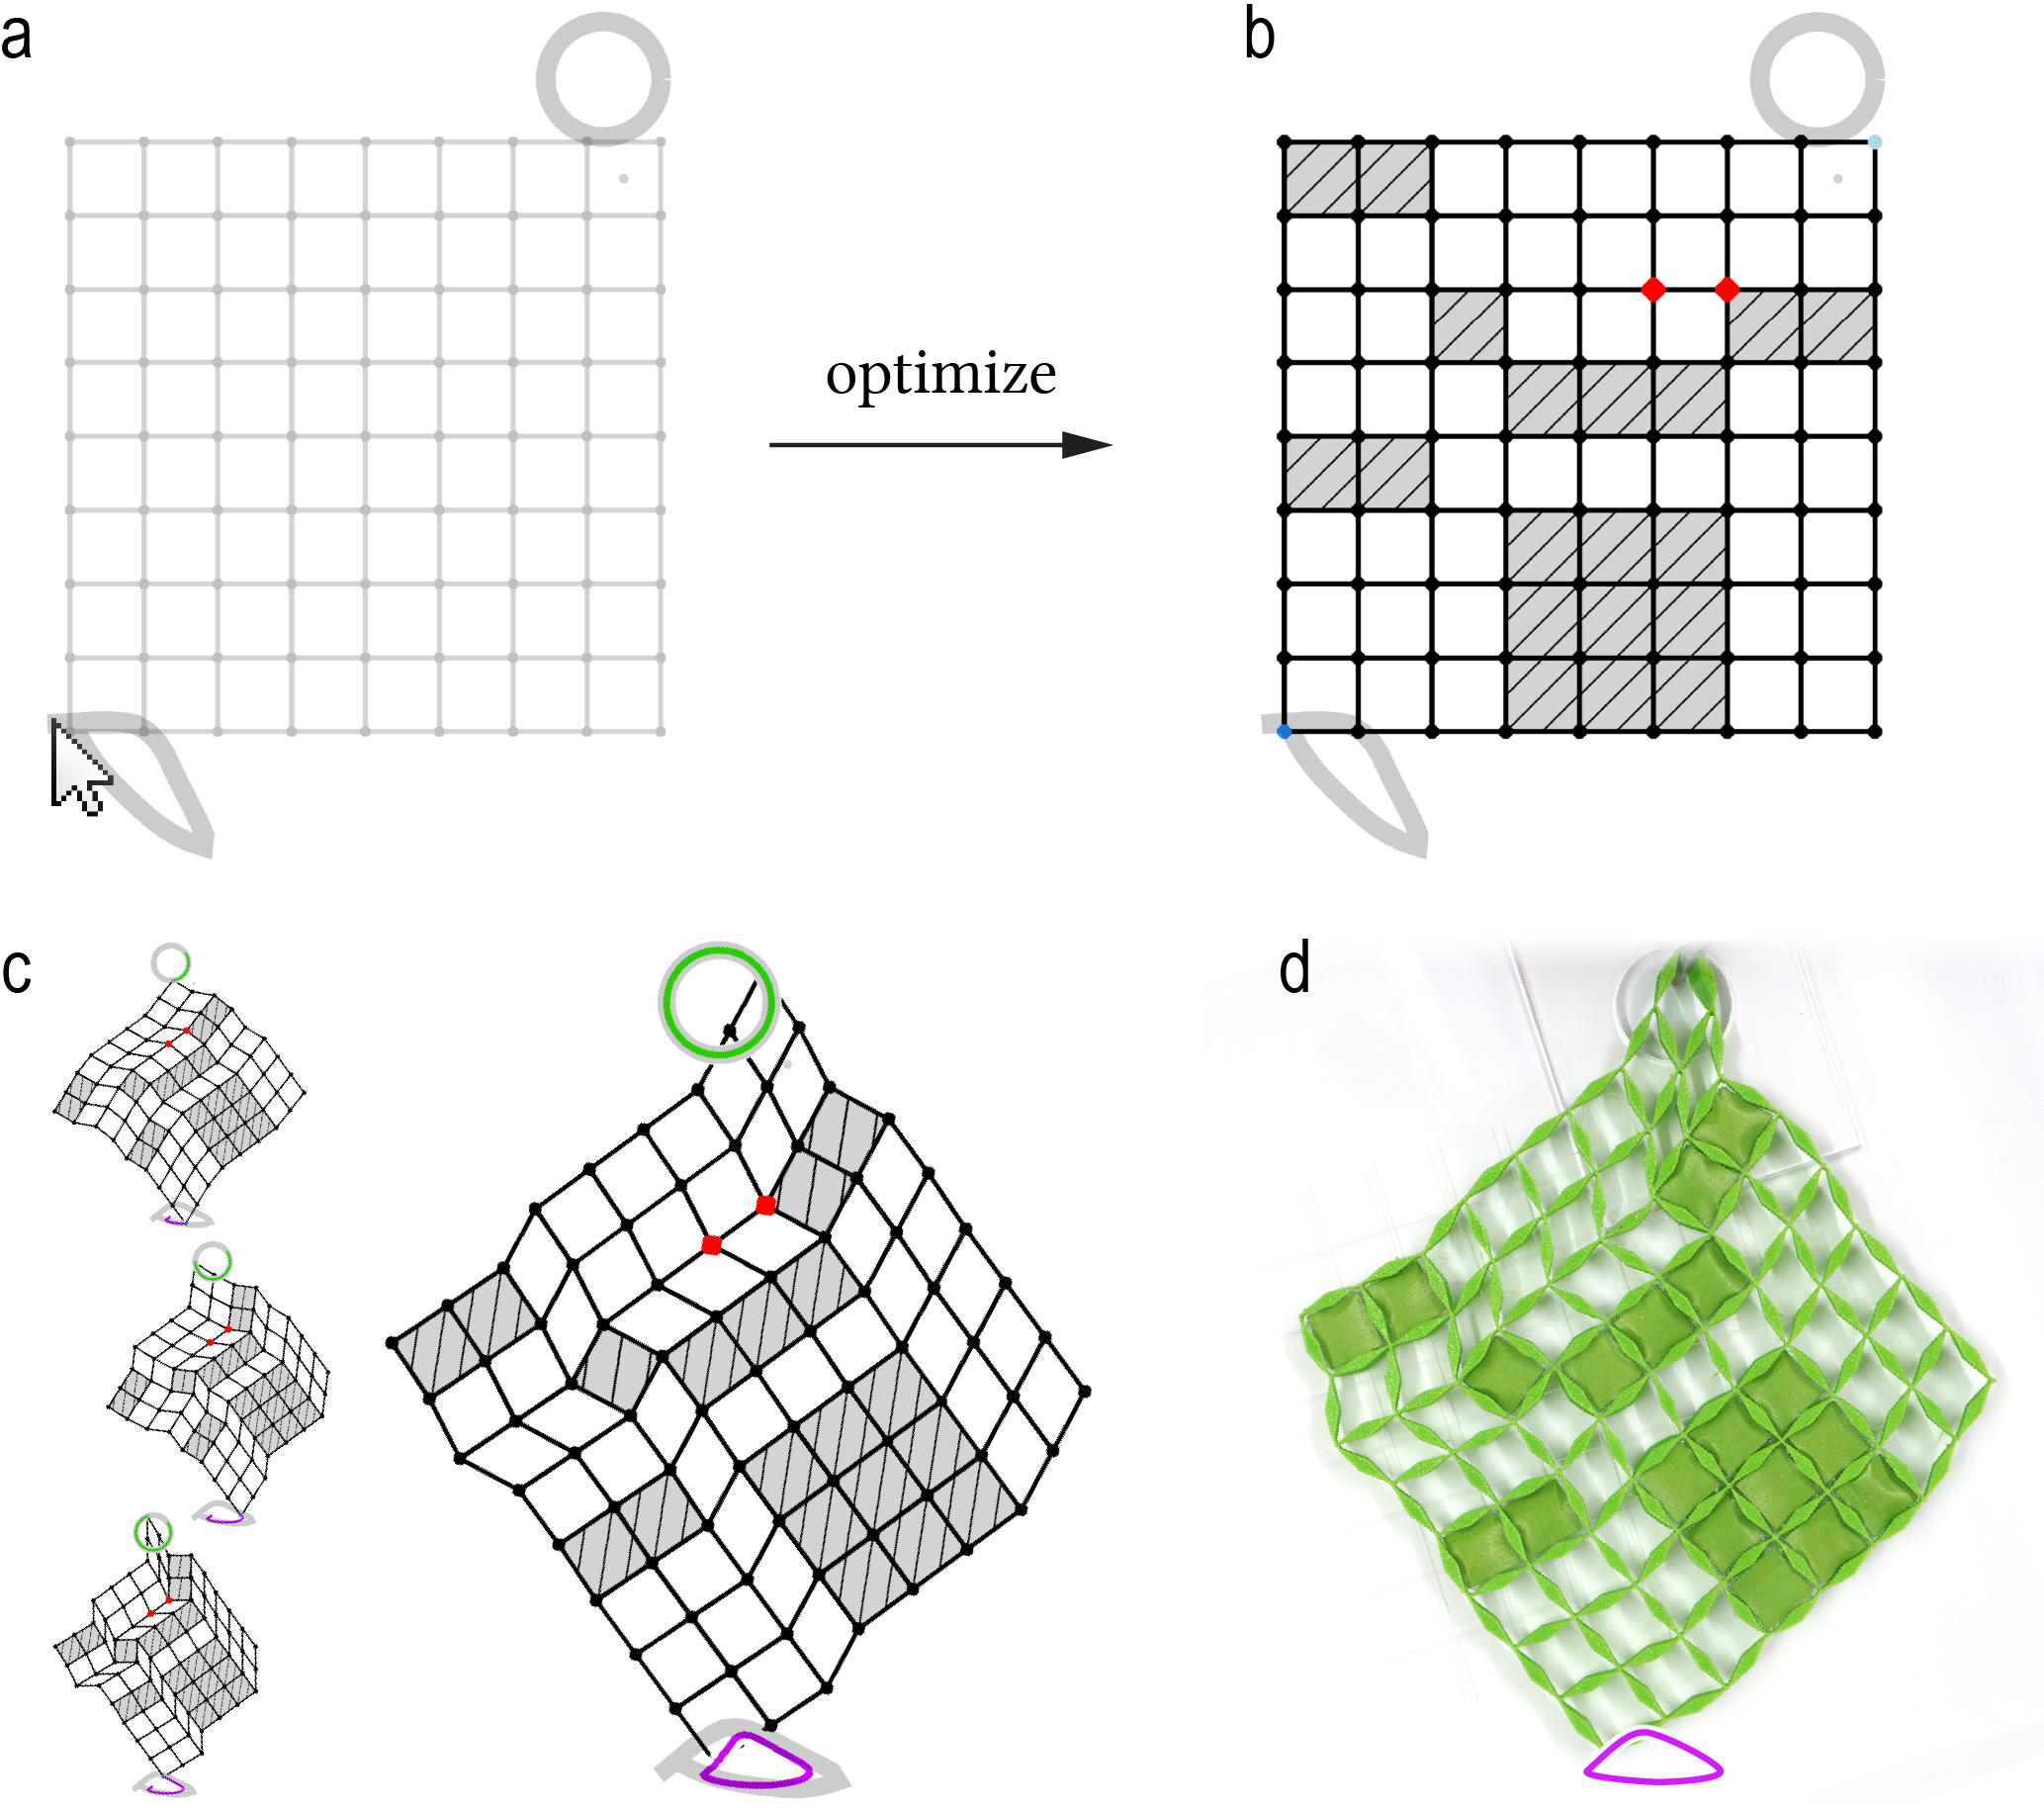
\includegraphics[width=\textwidth]{chapters/understanding-metamaterial-mechanisms-FIG/1-editor-and-walker.pdf}
    \caption[Short figure name.]{We define the underlying working principles of metamaterial mechanisms, which allows us to implement a computational design tool. (a) It takes user-drawn paths and (b) optimizes the cell configuration which implements the transformation. (c) In this example, we show the leg of a walker. (d) The fabricated result matches the optimized motion closely.
    \label{fig:1-editor-walker}}
\end{figure}


\section{Motivation \& challenges}

In this work, we set out to understand the underlying mechanisms that inform the design of metamaterial mechanisms. Such metamaterial mechanisms, as we introduced earlier in Chapter \ref{chapter:analog-metamaterials}, implement a transformation of an input movement to an output movement, such as in Figure \ref{fig:2-compare-doorlatch} with the retraction of the bolt when the door handle is pushed down.

\begin{figure} [h]
    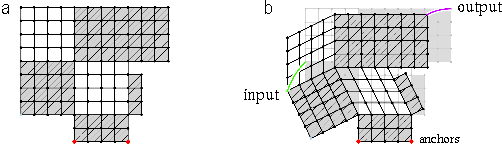
\includegraphics[width=\textwidth]{chapters/understanding-metamaterial-mechanisms-FIG/2-comparison-doorlatch.pdf}
    \caption[Short figure name.]{(a) Metamaterial mechanisms are implemented by their cell structure to create, e.g., this door latch, from a single block of material. (b) The microstructure implements a transformation from the green input path (pushing the handle) to the pink output path (retracting the bolt).
    \label{fig:2-compare-doorlatch}}
\end{figure}

Metamaterial mechanisms combine two types of cells on a regular grid. The individual cells (see Figure 3), are very simple---they are rigid or can shear. These cells are careful arranged within the material to play together in a well-defined way to implement the mechanism.

\begin{figure} [h]
    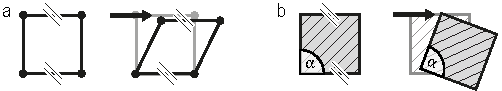
\includegraphics[width=\textwidth]{chapters/understanding-metamaterial-mechanisms-FIG/3-individual-cells.pdf}
    \caption[Short figure name.]{Metamaterial mechanisms consist of simple cells: shearing cells and rigid cells. (a) Shearing cells constrain their opposing edges to remain parallel and (b) rigid cells additionally maintain their angle.
    \label{fig:3-individual-cells}}
\end{figure}

In the remainder of this chapter, we will discuss metamaterial mechanisms on a higher level of abstraction, i.e., we will leave out the device applying the metamaterial and instead focus just on the cell structure and the transformation it implements.


\subsection{Understanding cell constraints and how they interact}

To achieve the movement that implements the desired mechanism, the cells need to be arranged on a grid to play together in a well-defined way. More formally, “play together” means that each individual cell has constraints that it propagates to its neighbors. For example, opposing edges of shear cells remain parallel (parallelism constraints) and rigid cells additionally maintain their angle (angle constraints). Since the cells are connected in two dimensions, their constraints can interact. We illustrate such constraint interactions in Figure \ref{fig:4-constraint-interaction}. This example shows how adding a single cell (marked in blue) prevents 7 other shear cells on the grid from shearing.

\begin{figure} [h]
    \includegraphics[width=\textwidth]{chapters/understanding-metamaterial-mechanisms-FIG/4-constraint-interaction.pdf}
    \caption[Short figure name.]{(a) In this example, (b) setting one cell rigid (c) prevents 7 cells from shearing, which changes the output drastically. (c) The green input path from (a) cannot be followed anymore.
    \label{fig:4-constraint-interaction}}
\end{figure}

\subsection{Large search space}
The example depicted in Figure \ref{fig:4-constraint-interaction} illustrates that interactions of constraints are unobvious and that by understanding them, we can reduce the search space drastically. We drill down on this example in Figure \ref{fig:5-large-search-space}. Here, the naive approach of simply swapping cell types to find a configuration that reaches a user-defined path results in $2^7=128$ equivalent mechanisms. This is because any changes within the 7 cells marked in orange (from Figure \ref{fig:4-constraint-interaction}) have no effect on the resulting mechanism. 

\begin{figure} [h]
    \includegraphics[width=\textwidth]{chapters/understanding-metamaterial-mechanisms-FIG/5-large-search-space.pdf}
    \caption[Short figure name.]{In this example, we have 128 configurations that all lead to the same mechanism, because the cell constraints interact. 
    \label{fig:5-large-search-space}}
\end{figure}

While this example only concerns with one specific scenario, the complete search space would be $2^{25} \approx 3\cdot {10}^7$. We generalize this in Section~\ref{section:search-space} and show how we reduce the search space by several orders of magnitude.


\subsection{Abstract representation reduces the search space}

The key insight of this work is to build an abstract representation of the cell constraints, which defines such distinct mechanisms. We encode constraints that edges impose on each other in a graph whose connected components define their degrees of freedom. We work directly in the reduced space of distinct mechanisms, which are defined by the connected components in the graph, rather than exploring the space of all possible cell configurations. 


\subsection{Computational design tool}

Our constraint-based representation of the metamaterial mechanism and the resulting reduction of the search space makes a computational design tool feasible. We present a computational design tool that optimizes a cell configuration for user-defined paths. Figure \ref{fig:1-editor-walker} shows how users define the size of the mechanism they are looking for and draw the input and output paths. Our heuristic optimization searches for a cell configuration that satisfies these boundary conditions. 


\subsection{Novel types of mechanisms}

With our computational approach, we not only ease the creation process for users, but we also discover new types of mechanical transformations that were not known before. Metamaterial mechanisms were manually designed to demonstrate useful mechanisms, such as a door latch or pliers. However, we show in Figure \ref{fig:6-compare-old-and-new-mechanisms} that the transformations they implemented were basic transformations, such as scaling. In this work, we demonstrate non-linear transformations, as illustrated in Figure 6b, such as self-intersections, oscillations and smoothing. We believe that the approach will foster more complex metamaterial mechanisms. 

\begin{figure} [h]
    \includegraphics[width=\textwidth]{chapters/understanding-metamaterial-mechanisms-FIG/6-compare-old-and-new-mechanisms.pdf}
    \caption[Short figure name.]{(a) The hand-designed mechanisms in only realize simple transformations. (b) In this work, we discover more complex and even non-linear transformations.
    \label{fig:6-compare-old-and-new-mechanisms}}
\end{figure}


\section{Contributions \& limitations}

Our main contribution is an understanding of the underlying mechanisms of metamaterial mechanisms. Understanding the constraints that interact within a grid enables a computational design tool that would otherwise not have been possible.

While the naive approach of swapping cells on the grid in order to find a cell configuration that implements a user-defined path transformation is computationally infeasible due to an exponentially growing search space, we contribute an abstract representation of the constraints. Our constraint graph representation reduces the search space significantly. 

We show that metamaterials can realize more complex and even non-linear mechanisms---a fact that was unknown before.

However, in this work, we focus on understanding the constraints on the most basic cells, i.e., the square shear and rigid cells. We do not explicitly implement rotated or pre-sheared cells, as suggested in Section~\ref{section:shear-cell}. Since the topology is the same, we show that our constraint graph applied to those cells as well. 


\section{Analysis of cell interactions}

The mechanisms we consider can exhibit intricate behavior even though they are built from very basic building blocks: shearing and rigid cells. Figure \ref{fig:4-constraint-interaction} already demonstrated how drastically a metamaterial can change after performing a small local change, e.g., swapping a shear cell for a rigid cell. These properties are non-obvious but crucial to understand.

In order to understand the movements of a mechanism, we need to simulate its physical behavior numerically. For larger grids the optimization procedure can be time consuming. This can hinder interactive exploration of the space of mechanisms and is especially problematic when sampling and simulating a lot of mechanisms to find one exhibiting some pre-defined behavior.

We describe how we model the constraints of a mechanism, which reduces the number of variables in the physical optimization from all grid points to a few edge vectors. This enables a significantly more efficient implementation and gives insights into the degrees of freedom of a mechanism.


\subsection{Understanding the constraints}
\label{section:graph}

Since our metamaterial consists of shearing and rigid cells, we observe two types of constraints in our cells: (1) parallelism constraints, such that opposing edges always remain parallel and (2) angle constraints, such that angles of rigid cells remain unchanged. Furthermore, all edges maintain their lengths. 
This means most edges cannot move independently, e.g. the same vector can represent edges that have to remain parallel. Edges that have to maintain a certain angle can also be represented by a reference edge that needs to be rotated in order to get the second one. To this end we build a constraint graph in which each node represents a cell edge and an arc between nodes the fact that one edge can be constructed by rotating the other (rotations also include the identity transformation).

Figure \ref{fig:7-single-cell-constraint-graph} illustrates the graph representation for each cell type individually. For shear cells, opposing cell edges always remain parallel. The constraint graph consequently only contains arcs between opposing cell edges. Figure \ref{fig:7-single-cell-constraint-graph}b illustrates that rigid cells are represented by a complete graph. This means that transforming one cell edge defines the transformation of all other edges. In other words, if we know how one edge is, e.g., rotated, we know the transformation of the entire cell, because opposing edges remain parallel and adjacent edges maintain their angle.

\begin{figure} [h]
    \centering
    \includegraphics[width=0.95\textwidth]{chapters/understanding-metamaterial-mechanisms-FIG/7-single-cell-constraint-graph.pdf}
    \caption[Short figure name.]{We model the constraints as graphs. (a) A shear cell is represented as 2 subgraphs that model the 2 independently moving adjacent edges and the parallelism constraint of opposing edges. (b) A rigid cell is a complete graph, showing that one edge defined the entire cell.
    \label{fig:7-single-cell-constraint-graph}}
\end{figure}


\subsection{Determining the degrees of freedom}

We think of the degrees of freedom (DoF) as a set of edge vectors that can be transformed independently. This property is also illustrated in Figure \ref{fig:7-single-cell-constraint-graph}, where the constraint graph of the shear cell in (a) consists of 2 connected components, which indicates that the cell has two independently moving parts, i.e., the green and blue edges. The rigid cell in (b) moves as a whole, thus the graph consists of one component. In general, the degrees of freedom of our metamaterial are simply defined by the number of connected components in the constraint graph.


\subsection{Building the constraint graph}

We build the entire constraint graph by connecting the constraints of single cells shown in Figure \ref{fig:7-single-cell-constraint-graph} to their neighbor cells, based on coinciding edges. For example, Figure \ref{fig:8-constraint-graph} shows how to proceed for a metamaterial with 4 cells. We start at the lower left cell and add its vertical edges to the constraint graph. The cell to the right shares the middle vertical edge, thus we link its other vertical edge to the graph, because they need to remain parallel. The two shear cells on the right are processed analogously.  The rigid cell, which cannot change its angle, effectively couples edges of the top right and lower left cell. Due to the parallelism constraints, entire rows and columns are linked. 

\begin{figure} [h]
    \includegraphics[width=\textwidth]{chapters/understanding-metamaterial-mechanisms-FIG/8-constraint-graph.pdf}
    \caption[Short figure name.]{We build the constraint graph by connecting the single cell constraints to their neighbor cells based on coinciding edges. 
    \label{fig:8-constraint-graph}}
\end{figure}

The notion of degree of freedom generalizes to entire mechanisms. The final graph in our example consists of 3 connected components, which tells us that the configuration has 3 DoF. Knowing one edge vector in each component uniquely determines all other edge vectors and thereby the whole mechanism. Therefore, we can formulate an optimization problem only involving 3 instead of 12 edges. We will provide details on this idea in Section~\ref{section:optimization}. 

In a cell grid that consists only of shear cells, the edges in each row and column represent one connected component each. The maximal number of degrees of freedom on an empty $n \times m$ grid is therefore $n+m$. Introducing a rigid cell joins the components of a row and a column into one, reducing the number of degrees of freedom by one.


\subsection{The influence of anchors}

So far, we only considered relative transformations of edges, i.e., edges are transformed with respect to each other. However, since the input of a mechanism is absolute, we need to fixate (i.e., anchor) the cell configuration in order to calculate the vertex positions in absolute space. 

Anchoring an edge in a cell configuration reduces its degrees of freedom by one. The same reasoning as for transforming edges, as discussed above, applies; since one edge of a connected component is defined (here, fixed to the ground), all edges in the component are defined. Furthermore, anchors define the scaling of an output path. As shown in Figure \ref{fig:9-anchor-effects}a, the length of the target paths is proportional to the distance between the anchors and the target vertices. Figure \ref{fig:9-anchor-effects}b illustrates, that anchors define a global rotation point.

\begin{figure} [h]
    \includegraphics[width=\textwidth]{chapters/understanding-metamaterial-mechanisms-FIG/9-anchor-effects.pdf}
    \caption[Short figure name.]{The anchor placement influences (a) the scaling of the output path and (b) the global rotation. 
    \label{fig:9-anchor-effects}}
\end{figure}


\section{Reducing the search space}
\label{section:search-space}

Since each cell on a $n\times m$ grid can have 2 states, rigid or shearing, we have $2^{nm}$ different possible configurations. However, not all configurations will generate a unique mechanism since shearing cells can become rigid because of the constraints. Consider the mechanism in Figure \ref{fig:10-non-shearing-constraint-graph}. The constraint graph reveals that the green and blue cells cannot shear. This is the case when \textit{all edges} of a cell are contained in the \textit{same connected component}. Since the rotation of both potentially independent edges of the shear cell are defined by the same connected component, their angle is constraint to the original 90° and can thus not shear.

\begin{figure} [h]
    \includegraphics[width=\textwidth]{chapters/understanding-metamaterial-mechanisms-FIG/10-non-shearing-constraint-graph.pdf}
    \caption[Short figure name.]{It might be non-obvious how many DoF this metamaterial has. Our constraint graph reveals that it contains 2 cells that cannot shear, i.e., the blue and the green one, leaving only 2 DoF.
    \label{fig:10-non-shearing-constraint-graph}}
\end{figure}

Since the blue and green cells cannot shear, the two cell configurations in Figure \ref{fig:10-non-shearing-constraint-graph} are equivalent. We only want to consider \textit{unique mechanisms} in our optimization. But how many of these unique mechanisms exist? To answer this question, we enumerate all possible connected component configurations. It is indeed possible to give an explicit formula for the number of all unique mechanisms on a $n \times m$ grid. 
We present the derivation of this function in Appendix \ref{appendix:unique-mechanisms}. Here, we show the empirical verification the formula for all configurations on grids with $n<5$. 
In Figure \ref{fig:11-search-space-reduction}, we show the number of all $2^{nn}$ mechanisms (gray) along with the number of unique mechanisms (blue). While this number still grows rapidly with increasing grid size it reduces the space of configurations on a grid from growing quadratically with respect to n in the log-plot to linearly, which is already significantly better. This enables us to consider much larger grids when searching for mechanisms with certain properties. 

\begin{figure} [h]
    \includegraphics[width=\textwidth]{chapters/understanding-metamaterial-mechanisms-FIG/11-search-space-reduction.pdf}
    \caption[Short figure name.]{The number of all configurations (log scale) on a square grid com-pared to the number of all unique mechanisms. 
    \label{fig:11-search-space-reduction}}
\end{figure}


\section{Simulating the motion}
\label{section:simulation}

To simulate the deformation of the object when a vertex of a cell moves, we use a simple elastic material model. We assume the edges are rigid and deformation occurs when two edges incident to a corner are rotated relative to each other. 

Through the constraint graph all edges are defined as soon as one representative edge per connected component is known. To define the remaining edges, we traverse the constraint graph, e.g. using breadth-first search, starting at the representative edge. When moving across an arc the appropriate rotation is applied. When all edges are known we can start to reconstruct cell vertices. To this end we traverse the grid itself starting at an anchored vertex. Each vertex is effectively reconstructed by summing all edge vectors along a path connecting the vertex to the anchor. 

Direct numerical simulation would try to find a set of grid vertices minimizing this deformation energy subject to a set of non-linear constraints, edges have to maintain their length, opposing edges in a cell have to stay parallel and angles in rigid cells stay at 90°. Additionally, certain vertices are fixed, either in their original position or by an external force driving the mechanism. 

Analyzing the constraint graph allows us to formulate a constrained optimization problem that has the same solution but is much more efficient than the direct approach.

The shape of the whole mechanism is determined by fixing the degrees of freedom, which requires two numbers per connected component. The current state of the deformation can therefore be modeled by a state vector $x\in\mathbb{R}^{2\ N_d}$ where $\ N_d$ is the number of degrees of freedom. Each state vector uniquely determines all edge vectors and is associated with the deformation energy

$$ D\left(x\right)=\sum_{i=0}^{N-1}\left(\alpha_i\left(x\right)-\frac{\pi}{2}\right)^2,$$

where $\alpha_i(x)$ stand for an interior angle of the i-th cell and $N$ for the number of cells. This energy models the fact that each cell will, depending on the material used, resist shearing, even for non-rigid cells. Note, that we only need to take one angle per cell into account because all angles in a cell produce the same energy. 

To simulate the deformation, we find a minimizer of $D$ with respect to the following constraints:

\begin{itemize}
	\item [C1.] The edges are rigid and therefore have to be fixed in length. Constraining all degrees of freedom to unit length will ensure this property for all edges in the mechanism.
	\item [C2.] Cells cannot invert, i.e., change their orientation. We therefore assure that the cell areas always remain positive.
	\item [C3.] Anchors are fixed in position.
    \item [C4.] The corner that is being dragged is fixed in position.
\end{itemize}
    
Note that we do not have to enforce that edges are parallel in shear cells or that rigid cells maintain their interior angles. These constraints are already built into the reduced representation and each state vector induces a valid cell layout. This constitutes another advantage over the direct approach where these constraints have to be taken into account explicitly.

Unfortunately, the energy and the constraints are non-linear and non-convex. However, the constraints are only quadratic and they can be analytically differentiated. The energy $D$ can also be analytically differentiated albeit yielding more complex terms due to the calculation of angles from edge vectors.
We solve the problem of minimizing $D$ subject to C1-C4 by employing the non-linear interior point solver IPOPT \cite{Waechter2006}, which gives us a configuration for a specific handle position. To simulate the full deformation, we sample the desired handle path and find the correct configuration by solving the optimization problem starting from the previous configuration as an initial guess.


\subsection{Invalid input}

The range of the handle corner is limited by the structure of the mechanism, which is fixed by anchors. If a handle position outside this range is prescribed the optimization problem has no solution because C4 cannot be satisfied. To yield an approximate result even for these situations we try to find a handle position, which is close to the desired one but in the range of the handle. To this end we solve another optimization problem minimizing the distance of the updated handle position ${\widetilde{P}}_h$ to the prescribed one $P_h$:

$$D\prime \left(x\right)=\left \| {\widetilde{P}}_h-P_h \right \|^2,$$

subject to the constraints C1-C3. The resulting configuration is one that is valid and places the handle close to the desired position. However, the solution represents only one valid configuration, which will not minimize $D$ in general. We therefore optimize $D$ with respect to C1-C4 using the new handle constraint.


\subsubsection{Evaluation}

As a preliminary evaluation of the simulation, we manually created 3 mechanisms with different inputs in our software and manufactured them from laser cut acrylic and 3D printed hinges (Ninjaflex filament). We tracked the motion of the physical mechanisms using OptiTrack with up to 7 markers on each mechanism and compared it with motion paths from our simulation. We adjusted the OptiTrack data to account for scaling. Figure \ref{fig:12-optitrack-evaluation} shows at one example that the recorded and simulated data matched closely. These experiments support that the results of our simulation match the behavior of physical mechanisms.

\begin{figure} [h]
    \includegraphics[width=\textwidth]{chapters/understanding-metamaterial-mechanisms-FIG/12-optitrack-evaluation.pdf}
    \caption[Short figure name.]{Example of our evaluation. The green path represents the paths from our simulation, blue is the data from OptiTrack.
    \label{fig:12-optitrack-evaluation}}
\end{figure}


\section{Optimization of cell patterns}
\label{section:optimization}

We aim to alleviate the problem of finding suitable configuration of cells given a set of desired input and output paths. In the following, we detail our algorithm that exploits aforementioned properties of metamaterials mechanisms such as the relation between cell transformation and anchors, and the constraint graph. Note that while most of our examples illustrate quadratic cell configurations, the approach is equally applicable for arbitrarily shaped objects. The main requirement for our approach is a simulation that correctly reproduces the deformation of a mechanism given an input path, like the one described in the previous section.

\subsection{Overview}

Our algorithm takes a set of user-defined input and output paths as well as a rough shape of the desired device as input. Our algorithm aims to find a close-to-optimal fit between the motion of the mechanism and the user-defined paths. Generally, input paths are actuated (e.g., by users) and the mechanism transforms this motion to the output path. In context of the optimization, however, we do not need to differentiate between input and output paths but use them as a list of paths which a mechanism should be able to reproduce. As a first step in our algorithm, we automatically determine the positions of the anchors for the cell configuration based on the scale and direction of the paths. We then generate a mechanism that produces the desired motion. An overview of the algorithm is illustrated in Figure \ref{fig:13-optimization-overview}.

\begin{figure} [!h]
    \centering
    \includegraphics[width=\textwidth]{chapters/understanding-metamaterial-mechanisms-FIG/13-optimization-overview.pdf}
    \caption[Short figure name.]{Overview of the process of automatically finding cell patterns given user-specified paths.
    \label{fig:13-optimization-overview}}
\end{figure}

Since the behavior of a mechanism is non-linear, we create cell configurations using stochastic optimization, specifically Simulated Annealing \cite{Ram1996, Kirkpatrick1983}. Instead of modifying the cell configuration directly, we modify the constraint graph, i.e., split and merge connected components until the algorithm converges. To speed up computation, we resort to a hierarchical approach where we first find an optimum configuration for scaled-down versions of the mechanism and use this configuration as seed for larger versions. The output of the algorithm is a cell configuration that produces the desired paths.


\subsection{Input and representation}

Users specify the shape of the cell configuration, denoted as $C_0\in{0,1}^{x,y}$, with $x$ and $y$ being the dimensions of the mechanism. This is a configuration of cells with undefined behavior. In the later optimization, the type of each cell is specified (e.g., they become shear or rigid cells), which ultimately governs the motion of the mechanism. Each mechanism is by its cells and its vertices $V$ and edges $E$. The position of the anchors $A\subseteq V$ governs the motion of a mechanism and fixes the mechanisms absolute position in space. Anchors are automatically determined by our algorithm.

Besides $C_0$, users specify a set of desired paths $P={P_0,\ P_1,\ldots,\ P_m}$. Each path is a list of points, stored as matrix $P_i\in\mathbb{R}^{2\times n}$. The first point $p_{i,0}$ of a path $P_i$ is a vertex of the cell configuration, i.e.,  $p_{i,0}\in V$. Note that while we use one input and one output path for clarity of exposure, the optimization generalizes to more than one input and output path.


\subsection{Setting anchors}

Our algorithm automatically determines candidates for positions of the anchors based on user-defined paths. This is done by anchoring a single edge $e$ (i.e., setting its two vertices to be anchors). There are three main considerations that govern the positioning of the anchors (i.e., finding which edge to anchor). First, the ratio between the length of paths should be similar to the ratio between the distance between individual paths and the anchors. As an example, if an input path is half the length of an output path (i.e., scale ratio 1:2), then the ratio for the distance between input path and anchors, and the output path and anchors should be similar. This accounts for scaling between the paths and can be calculated as

$$\min_l
{
\sum_{i=0}^{m}
\sum_{j=i+1}^{m}
{\frac{\left| P_i \right|}{\left| P_j \right|}}
-
{\frac{\left| e_l-P_i \right|}{\left| e_l-P_j \right|}}
}
$$

where $m$ denotes the number of user-defined paths. Secondly, anchors are essentially rotation points between paths. We therefore choose the location of anchors to reflect this rotation. Thirdly, to allow for maximum motion range of a path, the anchors should be as far ways from all path points as possible. This is formulated as 

$$\max_l{\sum_{i=0}^{s}\left|e_l-P_i\right|.}$$

Since this operation can be performed on a scale-down version of the configuration, we can exhaustively search the space and choose the best anchor positions. It is possible that no valid positions are found, e.g., if the length of a path exceeds to overall diagonal length of the cell configuration. If this is the case, users can adjust the paths, e.g., decrease the overall length of the paths.


\subsection{Generation of cell configurations}

Given a list of user-defined paths, any cell configuration $C$ will transform the paths in a specific way. For a single path $P_i$, this transformation is denoted as $C\left(P_i\right)$. We aim at finding a cell configuration $C_j$ with the minimal difference between $P_i$ and $C\left(P_i\right)$ while using as few as possible degrees of freedom to increase mechanical stability. We thus aim to find a solution (i.e., a close-to-optimal cell configuration) given the objective

$$\min_j{\sum_{i=0}^{m}{\omega_i \left| P_i-C_j \left( P_i \right) \right|.}}$$

$\omega_i\in\left[0,1\right],\ \ \sum_{i=0}^{m} \omega_i \mathrel{\mathop:}= 1$ 
are user-defined weighting factor for the individual paths. In our implementation, we typically use equal weights for input and output path (i.e., 0.5 for 2 paths).

A trivial approach to the problem would be to randomly sample cell configurations (i.e., switching cell types randomly) and choose the best fit between the user-defined paths and the paths the mechanism produces. This, however, is not feasible, as discussed in Section~\ref{section:search-space}, given the large number of possible cell configurations that yield similar movements or are rigid. 

In our approach, instead of modifying the cell configuration directly, we manipulate the underlying constraint graph with respect to the degrees of freedom of a configuration. We typically aim for a configuration with as little degrees of freedom as possible that still can reproduce a path well. A too low number of degrees of freedom would not allow for complex motion (e.g., with changes in direction). A too high number of degrees of freedom would lead to mechanically unstable structures. Therefore, we constrain a configuration to be within ${DoF}_{min}$ and ${DoF}_{max}$, which are typically chosen to be 2 and 5, respectively. 

For each step in our optimization, we compute the current degrees of freedom ${DoF}_j$ for a configuration $C_j$. The degrees of freedom govern the next step, i.e., if the next configuration shall contain more or less degrees of freedom. If the degrees of freedom should be increased, we split a chosen connected component. Conversely, we merge two connected components to decrease the degrees of freedom. If the degrees of freedom are within the limits, an operation is chosen randomly. The connected components that are affected by the operation are chosen randomly. 

We use Simulated Annealing for the optimization to avoid converging to a local minimum. We calculate the current temperature $T_j$ for each step as

$$T_k=(1+e^\frac{e_k}{T_0\alpha^k})^{-1},$$

where $e_k$ denotes the error of the current iteration $k$. It is calculated with respect the overall objects as the sum of differences between as user-defined paths, i.e. $e_k=\sum_{i=0}^{m}{\omega_i\left|P_i-C_k\left(P_i\right)\right|.}$ The error is normalized with respect to the length of the paths. $T_0$ is the starting temperature, which we typically choose as one third of the number of maximum iterations, as described below. $\alpha$ control the overall falloff of the algorithm, typically $0.85 < \alpha < 0.99$ (in our case, we chose $\alpha$ as $0.95$). To avoid that the algorithm converges in a local minimum, we restart the Simulated Annealing process several times. After each run, we compare the best results of the current and previous run. Converges is reached if the result did not improve compared to the previous run.


\subsubsection{Hierarchical generation}

We chose a hierarchical approach for the optimization, to avoid users having to estimate the cell resolution of their configuration. We start the Simulated Annealing process for an initial configuration $C_0$ with a small resolution r, e.g., 4 $\times$ 4 cells. Once the previously described Simulated Annealing procedure converged, we double the resolution and restart the Simulated Annealing with the larger resolution $r+1$. After convergence, we compare the error of the cell configuration $C_r$ and $C_{r+1}$. In case the result did not improve, we assume $C_r$ to be the best solution. If the result did improve, we increase the resolution again and restart the process. A typical error function for the whole process is shown in Figure \ref{fig:14-optimization-error-analysis}. Since the process typically converged after 100 to 150 iterations, we set the number of maximum iterations to 200. Similarly, the algorithm typically converges after increasing the resolution 2 to 3 times. We therefore set the maximum number of increasing the resolution to 5.

\begin{figure} [h]
    \includegraphics[width=\textwidth]{chapters/understanding-metamaterial-mechanisms-FIG/14-optimization-error-analysis.png}
    \caption[Short figure name.]{Typical error function for two examples. For top, the process con-verged after a total of 1400 iterations, with the minimum error for a resolution of 8 $\times$ 8 cells. Results with higher resolution (16 $\times$ 16) were discarded due to increased error. The bottom example converged with a resolution of 16 $\times$ 16 cells. For each resolution, Simulated Annealing is restarted multiple times.
    \label{fig:14-optimization-error-analysis}}
\end{figure}


\subsection{Evaluation}

We randomized a small number of ground truth examples to evaluate if the optimization finds an optimal solution given a user-defined input and output path. We randomly generated 10 cell configurations with 3 or 4 degrees of freedom. We manually set the input and output vertex, an input path and the anchors. Inputting this into the simulation yielded an output path. The input path and output path, as well as an empty low-resolution cell configuration with correct aspect ratio were given as input for the optimization. The resulting cell configurations, although different in terms of cell configuration and anchoring, could all truthfully reproduce the target movement. Two examples with target and solution are shown in Figure \ref{fig:15-groundtruth-test}. 

Note that the cell configuration, the anchors and the target resolution were not known to the optimization but were generated.

\begin{figure} [h]
    \includegraphics[width=\textwidth]{chapters/understanding-metamaterial-mechanisms-FIG/15-groundtruth-test.pdf}
    \caption[Short figure name.]{Two of ten ground truth examples (top) we used to test the optimization. The results in the bottom were generated without inputting the cell configuration or position of the anchors into the optimization procedure.
    \label{fig:15-groundtruth-test}}
\end{figure}


\subsection{Implementation}

While we already discussed the optimization and simulation in previous sections, we want to briefly mention the frameworks we used. We packed the metamaterial mechanism optimization, as described above, into a simple editor. The editor allows users to draw the shape of their desired mechanism and to set input and output paths, which the software will optimize for. Users can use pre-defined paths for precise motion constraints or simply draw rough paths. Time needed to generate a cell configuration depends on whether the solution requires a high-resolution configuration. If the solution is found in a low-resolution grid, the algorithm takes approximately 1 minute to converge on a commodity notebook (MacBook Pro 2015 with Bootcamp). For higher resolutions (e.g., 32 $\times$ 32 cells), finding the best solution takes up to 10 minutes. We are confident that we this time can be decreased by parallelizing parts of the algorithm, e.g., running multiple threads of Simulated Annealing at once. The editor is implemented in C\# and uses the .NET framework 4.5. We use the Windows Presentation Foundation (WPF) as our GUI toolkit. The optimization procedure is also implemented in C\#, which calls a wrapper to our C++ simulation tool. The simulation is written in C++, because it uses IPOPT \cite{Waechter2006}, as we discussed in Section~\ref{section:simulation}. We will provide the source code prior to the conference.

\subsection{Limitations of the design tool}

The editing capabilities of our editor are currently limited to 2D. Furthermore, we implemented only square cells so far. Triangular, rotated, or pre-sheared cells, as suggested in Section~\ref{section:shear-cell} are not integrated in the current version of the editor. However, this would be a simple extension.  We also currently don’t offer mesh export options, as we focused on the optimization. A conceivable option would be to implement the tool as a plugin to existing CAD tools, e.g., Autodesk Fusion 360, as they offer elaborate modeling options for the parts that embed the metamaterial.


\section{Examples}

The main contribution of this work is the abstract representation of metamaterial mechanisms, which ultimately allows an automatic generation of such metamaterials. While the device that embeds the metamaterial is not the focus of this work, we want to give some brief examples of how our generated metamaterials might be embedded in a device-context. This work allows to create new types of mechanisms, which experts of mechanism design can add to their repertoire. The examples here are merely intended to foster future discussion and research of monolithic cell-based mechanisms. More transformations are listed as examples in Appendix \ref{appendix:example-transformations}.

\paragraph{Kinetic sculptures.} One example, where metamaterial mechanisms might be embedded into, are kinetic sculptures, toys, or walking automata \cite{Thomaszewski2014}. As shown in Figure \ref{fig:16-examples-walker}, our design tool enables users to create custom walk-cycles from metamaterials. 

\begin{figure} [h!]
    \includegraphics[width=\textwidth]{chapters/understanding-metamaterial-mechanisms-FIG/16-examples-walker.pdf}
    \caption[Short figure name.]{Embedding metamaterial mechanisms into kinetic sculptures. 
    \label{fig:16-examples-walker}}
\end{figure}

\paragraph{Custom mechanisms.} Users might also want to create grippers with a custom motion path. In Figure \ref{fig:17-examples-gripper}, we illustrate embedding metamaterial mechanisms with different motion paths as grippers for collecting items, e.g., for picking-challenge robots. Other applications for such custom paths that come to mind are, e.g., fans with a path cycle, or deflectors for sprinkler which can be customized to sprinkle a specific area optimally.

\begin{figure} [h!]
    \includegraphics[width=\textwidth]{chapters/understanding-metamaterial-mechanisms-FIG/17-examples-gripper.pdf}
    \caption[Short figure name.]{Example of metamaterial mechanisms as gripper with custom motions for, e.g., robots.
    \label{fig:17-examples-gripper}}
\end{figure}

\paragraph{Clock.} Another simple example is an alarm clock, as depicted in Figure \ref{fig:18-examples-oscillating-clock}. The metamaterial transforms a rotary input into an oscillating motion to strike the bells.

\begin{figure} [h!]
    \includegraphics[width=\textwidth]{chapters/understanding-metamaterial-mechanisms-FIG/18-examples-oscillating-clock.pdf}
    \caption[Short figure name.]{A simple example is embedding an oscillating metamaterial into an alarm clock.
    \label{fig:18-examples-oscillating-clock}}
\end{figure}


\section{Discussion \& outlook}

Our work aims at providing an understanding of metamaterial mechanisms and go beyond purely exploratory work. Our work opens way for researchers to explore, build and use such mechanisms. Moving away from a representation that is based on cells to a higher level---the constraint graph---allowed us to significantly reduce the space of cell configurations, making computational approaches feasible. Note that while the search space is highly reduced, it is still not feasible to fully enumerate the space. As discussed above, a cell configuration of 9 $\times$ 9 cells yields $10^{12}$ unique transformations (but $10^{24}$ cell configurations). We are confident, however, that our work informs the research in the space and can provide a foundation to make metamaterial mechanisms accessible to a broader audience. 


\subsection{Limitations and considerations}

The constraints graph and the optimization allow us to generate insights into the inner workings of metamaterial mechanisms and create a computational tool that allows for their automatic generation. There are, however, limitations to our approach.

\subsubsection{Transformation symmetry}
For a given cell configuration, moving an input vertex along the input path yields a transformation of the output vertex, resulting in an output path. If, however, the output vertex is moved along the same output path, the transformation of the input vertex is not equal to the input path. This behavior has to be taken into account when designing mechanisms that should be actuated from by moving the input and the output vertex. It can, however, also be exploited to create more interesting and complex mechanisms.

\subsubsection{Transformation complexity}
In our experiments, we observed that transformation between an input and an output path are limited in their complexity. Specifically, we saw that the number of inflection points between the two paths is roughly the same. An input path with one inflection points, for example, usually yields output paths with zero to two inflection points, but not arbitrary number. 

\subsubsection{Error cases of the optimization}
While the optimization generally yields good results, there are cases where no solution (i.e., no good cell configuration) can be found. Examples include a mismatch in complexity between input and output path (e.g., line as input and an ampersand curve as output), or when input and output are close together but face into different direction. We will alleviate this problem by warning users of impossible configuration before the optimization. 

\subsubsection{Extending to 3D mechanisms}
The constraint graph is based on the fact that a cell that is constraint in length is fully defined by a single angle. This does not hold true for 3D cell configurations. Therefore, there is no trivial extension of our approach into the 3rd dimension. We already started investigating this interesting future work, including replacing the 2D angle constraint with using the angles of a basis in each cell as constraints. A preview of a deformed 3D mechanism with 2 rigid cells is shown in Figure \ref{fig:19-3D-grid}.

\begin{figure} [h]
    \centering
    \includegraphics[width=0.65\textwidth]{chapters/understanding-metamaterial-mechanisms-FIG/19-3D-grid.png}
    \caption[Short figure name.]{Preview of a 3D deformed mechanism with 2 rigid cells.
    \label{fig:19-3D-grid}}
\end{figure}


\subsection{Practical extensions}

There are several practical extensions to our work, that concern the editor, including the simulation and generation of mechanisms. 

\subsubsection{Adapt to material properties}
We used an idealized simulation that does not incorporate engineering factors such as material properties or friction. We did so to focus on the interaction between geometric constraints within a mechanism, which could be missed when taking mechanical factors such as transmission loss into account. While the mechanical properties can be optimized (e.g., through high-resolution 3D printing), the underlying constraints are inherent to the geometry. Material properties could be used to expand the repertoire of transformations. Including other types of simulation such as finite element analysis would be one beneficial extension of the editor. This would also allow us to adaptively change the stiffness, thus actuation force, of a mechanism. This can be achieved by merging cells.

\subsubsection{Multiple layers with the same input}
Many practical applications such as a multi-legged Jansen walker or a robotic gripper require that multiple layers of mechanisms move in concert with each other, i.e., they use same coinciding input.  While our current editor only supports a creating a single layer at a time, they could be merged using any CAD tool.

\subsubsection{Extending to different cell types}
Our constraint graph, and consequently our optimization algorithm, hold true for other cell suggested previously in Section~\ref{section:shear-cell}, such as rotated and pre-sheared cells. Our editor only needs to be extended slightly to edit such cells.
 
\begin{figure} [h]
    \centering
    \includegraphics[width=0.9\textwidth]{chapters/understanding-metamaterial-mechanisms-FIG/20-generalized-2D-constraint-graph.pdf}
    \caption[Short figure name.]{Our constraint graph generalizes to the cells we introduces in Section~\ref{section:shear-cell}.
    \label{fig:20-generalized-2D-constraint-graph}}
\end{figure}

\subsubsection{Considering temporal changes}
We were concerned with the spatial transformation of metamaterial mechanisms. An extension of the optimization would be to also include a temporal component. Considering the speed of transformation would allow features such as keyframing and easing of motion. We plan to investigate this interesting aspect by adapting our error function and add keyframing to the editor.


\section{Conclusions}

We analyzed metamaterial mechanisms with respect to their topological constraints. Although the basic cells in this work (shear and rigid cells) are simple, connecting them creates complex interactions. We investigated these interactions, which we modeled as a constraint graph. This abstract graph representation allows us to explore metamaterials on a more abstract level and avoid having to rely on the raw cell structure which exhibits a prohibitively large search space. Consequently, we implemented our knowledge as a computational design tool for the automatic generation of such mechanisms. 

On a higher level, we think of our work as the first step towards what we like to call \textit{heterogenous mechanical metamaterials}. We define them as metamaterials that consist of \textit{different types} of cells. Most often metamaterials consist of cells that are topologically equivalent; all cells have the same function, but they can vary in parameter. Metamaterial mechanisms is one example of a material that consists of \textit{topologically different cells}. They exhibit interesting behavior yet the interactions between cells are hard to understand. In the future, we will go step-wise towards investigating more of these heterogenous metamaterials by creating generic tools that allow researchers to investigate combinations of different types of cells from related work. 


\pagebreak

\section{Appendix A: Enumerating all unique mechanisms}
\label{appendix:unique-mechanisms}

As noted in Section~\ref{section:search-space}, all edges in a row or column necessarily belong to a single connected component. Starting with an empty $n \times m$ grid we have $n+m$ connected components. Introducing a rigid cell joins two connected components and removes one degree of freedom. Suppose we want to enumerate all unique mechanisms with $k$ degrees of freedom. This amounts to $k$ connected components where we differentiate between $x$ empty columns, $y$ empty rows and $z$ components formed by merging rows and columns using rigid cells. There are $\binom{n}{x}$ ways to choose the columns and $\binom{m}{y}$ ways to choose the rows. The remaining $m-y$ rows and $n-x$ columns can be arbitrarily partitioned into $z$ sets. The Stirling number of the second kind counts the number of these partitions as $S(n-x,\ z)$ and $S(m-y,z)$ where we use the convention $S\left(a,b\right)=0$ for $a<b$. The $z$ sets of rows and columns can be connected in $z!$ ways. This gives 
$$G^{n,m}\left(x,y,z\right)=\ \binom{n}{x}\ \binom{m}{y}S\left(n-x,\ z\right)\ S\left(m-y,z\right)\ z!$$
different possibilities. Summing over all values for $x,\ y$ and $z$ we obtain the number of all possible unique mechanisms on a $n \times m$ grid. We empirically verified this number by analyzing all possible configurations on grids with $n<5$.

\pagebreak

% \appendix

\section{Appendix B: Example transformations}
\label{appendix:example-transformations}
\begin{figure} [h!]
    \includegraphics[width=\textwidth]{chapters/understanding-metamaterial-mechanisms-FIG/21-optimization-results.pdf}
    \caption[Short figure name.]{Examples of auto-generated metamaterial mechanisms.
    \label{fig:21-optimization-results}}
\end{figure}


% \begin{figure} [h]
%     \includegraphics[width=\textwidth]{chapters/understanding-metamaterial-mechanisms-FIG/}
%     \caption[Short figure name.]{
%     \label{fig:}}
% \end{figure}
% \chapter{Integrating mechanical computation into custom objects}
%\chapter{Processing digital signals}
\chapter{Digital mechanical metamaterials}
\label{chapter:digital}

% \todo{
% similar to our work on digital, based on \\
% Zanaty2018: Programmable Multistable Mechanisms: Synthesis and Modeling\\
% Merkle1993: Two Types of Mechanical Reversible Logic
% }

% \todo{add to DIGITAL for recharging: Wu2018 - Metastable modular metastructures for on-demand reconfiguration of band structures and nonreciprocal wave propagation}


% \todo{write transition from talk: stiffnes ratio, decay, ...}


% Personal fabrication machines, such as 3D printers, allow users to make custom objects. While early work on 3D printing revolved around designing the outside of such objects [24, 32], recently researchers started exploring 3D printing as a means to design the \textit{inside} of objects. Applications include moving objects’ centers of gravity so as to make them stand [20] or spin [1].

% Pushing this further, researchers created objects that consist internally of a large number of 3D cells arranged on a regular grid [15]. Since each cell is designed to perform a specific deformation, objects that entirely consist of such cells literally offer thousands of degrees of freedom. Such structures are also known as \textit{metamaterials} [18].

% While metamaterials were initially understood as materials, we recently proposed to think of them as \textit{machines}; such metamaterial mechanisms [10] consist of a single block of material, the cells of which play together in a well-defined way in order to achieve macroscopic movement. We used this principle previously to implement simple mechanical objects, such as a door latch (\todo{Figure 7}).

Metamaterial mechanisms, like all \textit{analog} machines, are limited in terms of complexity. As forces are passed on from one cell to the next, they are damped and the activation energy dissipates, which causes the mechanical ``signal" to decay exponentially. This limits the number of mechanisms that can be concatenated and therefore the complexity of the machine.

In this work, we explore how to extend this concept towards \textit{digital} mechanisms. Combining metamaterial mechanisms with concepts from mechanical computing and mechanical signal propagation \cite{Raney2016, Nadkarni2014}, we introduce a new type of cell that propagates a digital mechanical signal, i.e., it counteracts signal decay and thus allows signals to pass through an arbitrary number of cells. We extend this basic mechanism to implement simple logic functions. 

To illustrate this concept, Figure \ref{fig:1-door-lock} shows a combination lock implemented using digital metamaterials. The device offers ten digit buttons on the front. Users tap these buttons to enter their code, then press the `open' button to unlock the door. 

\begin{figure} [h]
    \includegraphics[width=\textwidth]{chapters/digital-metamaterials-FIG/1-door-lock.pdf}
    \caption[Short figure name.]{(a) This combination door lock is implemented as a \textit{digital mechanical metamaterial}, i.e., a single block of material based on a regular grid of cells. It allows users to input a numeric code, it processes the code, checks its correctness, and unlocks the latch. (b) Under the hood, the lock consists of an array of cells that transmit and process a mechanical signal. 
    \label{fig:1-door-lock}}
\end{figure}


\section{Basic cells of digital mechanical metamaterials}

Digital metamaterials are based on a new type of cell that propagates a mechanical signal reinforced by an embedded bistable spring. 


\subsection{The bit cell is the main underlying mechanism}

Figure \ref{fig:2-bit-cell} shows the key element behind digital metamaterials, which we call \textit{bit cell.} Bit cells contain a bistable spring, which allows them to take on two discrete states. Figure \ref{fig:2-bit-cell}a shows the bit cell in its \textit{tense state.} (b) When triggered, the spring discharges, causing the cell to switch from its \textit{tense} state to its \textit{relaxed} state.  

\begin{figure} [h]
    \includegraphics[width=\textwidth]{chapters/digital-metamaterials-FIG/2-bit-cell.pdf}
    \caption[Short figure name.]{(a) When triggered, this \textit{bit cell} changes its state from tense to (b) relaxed.
    \label{fig:2-bit-cell}}
\end{figure}

As shown in Figure \ref{fig:3-ports-at-cell}, bit cells feature an input port and output port. A mechanical impulse that reaches the input port triggers the cell, which creates an impulse at the output port. Because discharging the spring releases mechanical energy, the impulse at the output port is larger than the required trigger impulse at the input port.

\begin{figure} [h]  
    \includegraphics[width=\textwidth]{chapters/digital-metamaterials-FIG/3-ports-at-cell.pdf}
    \caption[Short figure name.]{Bit cells offer an input and an output port.
    \label{fig:3-ports-at-cell}}
\end{figure}

As illustrated by Figure \ref{fig:4-signal-transmission}, this allows us to concatenate bit cells in a way that allows cells to trigger their immediate neighbors, resulting in a simple signal propagation mechanism similar to \cite{Raney2016}.

\begin{figure} [h]  
    \includegraphics[width=\textwidth]{chapters/digital-metamaterials-FIG/4-signal-transmission.pdf}
    \caption[Short figure name.]{Concatenating bit cells creates a signal transmission. (a) Initially all bit cells are in their tense position. (b) Triggering the leftmost cell causes the signal to propagate through all cells from left to right.
    \label{fig:4-signal-transmission}}
\end{figure}

\subsection{The combination lock example}

Bit cells and the resulting concept of signal propagation allow us to implement a hierarchy of digital mechanisms of increasing complexity. We discuss these logic functions and mechanisms in full detail later in this paper, as well as a simple manual recharge mechanism to set discharged springs back into their tense state. However, Figure \ref{fig:5-elements-in-the-door-lock} provides a rough overview of the different elements that implement the combination lock.

\begin{figure} [h]  
    \includegraphics[width=\textwidth]{chapters/digital-metamaterials-FIG/5-elements-in-the-door-lock.pdf}
    \caption[Short figure name.]{Our door lock consists of 82 cells, which implement the signal transmisison, the evaluation of each digit input by the user, an AND gate, and one amplifier cell with a pre-amplification step to move the blocking bolts sufficiently.
    \label{fig:5-elements-in-the-door-lock}}
\end{figure}

(1) To input the code, users tap one of the digit buttons on the front, which changes the state of the \textit{digit evaluation} cells. The device contains 10 of these---one for each possible digit. (2) When the user pushes the `open' button, three signal transmission lines are set off simultaneously; two of which run through the digit evaluation units and (3) set the state of the \textit{AND gate.} The AND gate evaluates the correctness of the code by computing a logical AND the two rows of digits input by the user. The third signal transmission line runs from the bottom left towards the right, around the corner, and upwards where (4) the signal is \textit{bifurcated.} This allows triggering (5) a double-sized \textit{amplifier cell} that actuates the bolts to unblock the door.

Figure \ref{fig:6-bolts} shows a close-up of these bolts. (a) As long as the bolts are in place, they prevent the shearing cells in the middle from shearing, thereby blocking the door. (b) When the bolts are retracted, the shearing cells can shear and pushing down the handle retracts the latch---as we discussed in Chapter \ref{chapter:analog-metamaterials}. This is where our digital metamaterials connect to the analog metamaterial door latch mechanism.

\begin{figure} [h]  
    \includegraphics[width=\textwidth]{chapters/digital-metamaterials-FIG/6-bolts.pdf}
    \caption[Short figure name.]{We effectively lock the latch mechanism by stiffening the shearing area that enables it. We do so by inserting bolts. Once users entered the key code correctly, our lock signal retracts the bolt and enables the latch mechanism.
    \label{fig:6-bolts}}
\end{figure}


\section{Contribution, benefits and limitations}

Our main contribution is the concept of digital mechanical metamaterials. They allow integrating computational abilities into the structure of 3D printed objects. We provide a modular system consisting of digital cells (hardware) and an editor (software) that provides a toolkit to users, enabling them to create new digital mechanisms. 

While analog metamaterial mechanisms are subject to damping, which causes the mechanical ``signal" to decay exponentially and limits the number of `steps' that can be performed, \textit{digital} mechanical metamaterials enable transmitting signals through an \textit{arbitrary} number of cells. 

When we contrast digital mechanical metamaterials to the traditional approach of augmenting objects with electronic microcontrollers, sensors, and actuators \cite{Savage2014}, our approach results in an entirely mechanical solution and can be produced entirely using a 3D printer. However, since our approach lacks loops, clocks, and memory, our approach is limited to much simpler devices.


\subsection {Scope of this concept}
% \todo{add scope to set expectations right: schaltnetz vs schaltwerk, is turing complete?}

This work, more than the other works in this thesis, is a thought experiment, a what-if question, rather than a potential solution to a potential problem. Our digital metamaterials are by no means intended to replace computers. We aimed to investigate the question, whether the habit of using microcontrollers for very simple evaluation or computations is really necessary, or if we can perform simple operations within the metamaterial structure.  

The scope of our current implementation spans \textit{combinational circuits} (ger. Schaltnetz). Our cell-based material can perform any combinational logic, as we will demonstrate a NAND gate in Section \ref{section:digital-gates}. Furthermore, like combinational circuits our metamaterials present time-independent logic, i.e., the output is a pure function of the present input only.

This work could be expanded to sequential circuits (ger. Schaltwerk) by engineering a protected region that is unaffected by the recharging action and can thus act as memory, and by introducing an external clock signal. 



\section{Signal processing based on cells}

\subsection{Routing signals}

In this and the following section, we now show the individual cells that implement the combination door lock we showed in Figure \ref{fig:5-elements-in-the-door-lock}. We begin with the cell types that allow us to route signals through 3D objects. We already looked at signal propagation along a straight line (Figure \ref{fig:4-signal-transmission}); in this section, we demonstrate how to route signals around corners, across other signal lines, and how to bifurcate signals. 

Routing signals is important because 3D printed objects can have arbitrary shape and routing allows transmitting a signal from where it emerges to where the information is needed. For the door lock, for example, we route users input from the digit inputs to the door latch mechanism---which is located elsewhere in our object.

The more specialized routing cells are all based on \textit{bit cells.} However, we position their output ports to be oriented towards the neighbor cell we want to trigger. So while the bit cells in Figure \ref{fig:4-signal-transmission} feature an output port on the side opposite to the input port, the cell shown in Figure \ref{fig:8-simulation-tear-and-rotate} redirects the signal by 90° by adding a beam to the arm of our bistable spring. This beam rotates with the arm of the spring, allowing it to tap the input port of the rotated cell on the top right.

\begin{figure} [h]  
    \includegraphics[width=\textwidth]{chapters/digital-metamaterials-FIG/8-signal-redirecting-90deg-2D.pdf}
    \caption[Short figure name.]{We use a new type of output port to redirect the signal by 90°. We exploit the rotational movement of the spring and attach a beam that taps its neighboring cell.
    \label{fig:8-signal-redirecting-90deg-2D}}
\end{figure}

As illustrated by Figure \ref{fig:9-siganl-redirecting-90deg-3D}, we can route signals in 3 dimensions by concatenating multiple such mechanisms. Here we route the signal from the x/y plane to the x/z plane to the y/z plane. 

\begin{figure} [h]  
    \includegraphics[width=\textwidth]{chapters/digital-metamaterials-FIG/9-siganl-redirecting-90deg-3D.pdf}
    \caption[Short figure name.]{(a) Rotating the receiving cell allows us to redirect signals from one plane to another. (b) Concatenating three assemblies allows us to route signals in 3D. 
    \label{fig:9-siganl-redirecting-90deg-3D}}
\end{figure}

Figure \ref{fig:10-signal-crossing} shows a specialized three-cell mechanism that allows two signals to pass each other in minimal space. We use a crossbar that reaches from the output port of the left cell to the input port of the right cell that spans across the middle cell.

\begin{figure} [h]  
    \includegraphics[width=\textwidth]{chapters/digital-metamaterials-FIG/10-signal-crossing.jpg}
    \caption[Short figure name.]{We cross signals by running a crossbar across another cell.
    \label{fig:10-signal-crossing}}
\end{figure}

Figure \ref{fig:11-signal-bifurcation} shows two mechanisms that bifurcate signals. The design shown in (a) triggers two parallel signal lines. The design shown in (b) triggers two signal lines oriented in opposite directions. Both designs exploit the fact that our bistable springs require less energy to be triggered than they output, which allows triggering two cells from one. 

\begin{figure} [h]  
    \includegraphics[width=\textwidth]{chapters/digital-metamaterials-FIG/11-signal-bifurcation.pdf}
    \caption[Short figure name.]{We can bifurcate signals (a) in a parallel manner or (b) let the two signals run in opposite directions. 
    \label{fig:11-signal-bifurcation}}
\end{figure}

Figure \ref{fig:12-signal-merging-OR} shows how we merge two signals. This is an interesting construct, because it implements an OR gate.

\begin{figure} [h]  
    \includegraphics[width=\textwidth]{chapters/digital-metamaterials-FIG/12-signal-merging-OR.jpg}
    \caption[Short figure name.]{We use the opposite assembly to merge signal as we did to bifurcate them. This implements an OR gate.
    \label{fig:12-signal-merging-OR}}
\end{figure}


\subsection{Logic functions}

To implement logic functions, we need to go beyond merely transmitting signals to also evaluating signals, which we achieve by blocking them. In the combination lock from Figure \ref{fig:5-elements-in-the-door-lock}, we block signals for wrong digit inputs so that the door stays blocked. Later in this section, we present cell arrangements that implement basic logic, such as AND or NAND.

\subsubsection{Blocking signals using gate cells}

To allow for asynchronous input, we have designed cells capable of storing the first input that reaches them and do not act until the last signal has been received. We call these cells \textit{gate cells.} Our approach is based on rod logic \cite{Merkle1993}. 

As illustrated by Figure \ref{fig:13-gate-cells-illustration}a these cells work by placing a ``blocker" across their neighboring cell. When the cell on the right is triggered before the cell on the left, the blocker is aligned with the output port of the right cell so that it cannot pass and signal is blocked. However, triggering the left cell, as shown in Figure \ref{fig:13-gate-cells-illustration}b, moves the blocker out of the way and the signal can pass through. The position of the blocker can also be defined to initially let signals through and only after actuation to block signals, as shown in Figure \ref{fig:13-gate-cells-illustration}c-d.

\begin{figure} [h]  
    \includegraphics[width=\textwidth]{chapters/digital-metamaterials-FIG/13-gate-cells-illustration.pdf}
    \caption[Short figure name.]{\textit{Gate cells} validate signals and can be configures to block signals (a-b) or let signals pass (c-d) in their tense state.
    \label{fig:13-gate-cells-illustration}}
\end{figure}

Figure \ref{fig:14-signal-blocking} shows the design of the two cells that form the gate cell. Each crossbar has a blocker attached on its underside.

\begin{figure} [h]  
    \includegraphics[width=\textwidth]{chapters/digital-metamaterials-FIG/14-signal-blocking.JPG}
    \caption[Short figure name.]{We position a blocking element that is intended to either block the signal output or let it pass.
    \label{fig:14-signal-blocking}}
\end{figure}


\subsubsection{Logic functions based on gate cells}

We can concatenate multiple gate cells to create combinational logic functions. Figure 15 uses simplified symbols to illustrate how the positions of the blockers are configured to implement the function $A\ {\land}\ {\neg}B\ {\land}\ C\ {\land}\ D\ {\land}\ {\neg}E$. The positive input cells A, C, and D need to be triggered to move the blocker out of the way and let the signal pass. The negated inputs B and E are implemented by positioning the blocker so that they let the signal pass when they are \textit{not} triggered and block the signal otherwise.

If we rename the inputs of the logic function that is shown in Figure \ref{fig:15-code-evaluation-1--5} from A--E to 0--4, it implements a 5-digit code evaluation. To implement the combination lock with 10 digits, we add a second row of inputs. Now we have two logic functions (one in each row), which both need to be correct, thus we add an AND gate. Figure \ref{fig:16-code-evaluation-0--9} illustrates that the key code is `0 2 3 8'. 

\begin{figure} [h]  
    \includegraphics[width=\textwidth]{chapters/digital-metamaterials-FIG/15-code-evaluation-1--5.pdf}
    \caption[Short figure name.]{(a) When all inputs are tense, the signal cannot pass. (b) Triggering the correct inputs, here A, C, and D, moves the blockers so that the signal can pass.
    \label{fig:15-code-evaluation-1--5}}
\end{figure}

\begin{figure} [h]  
    \includegraphics[width=\textwidth]{chapters/digital-metamaterials-FIG/16-code-evaluation-0--9.pdf}
    \caption[Short figure name.]{We add an AND gate to validate the two rows that yield the 10-digit.
    \label{fig:16-code-evaluation-0--9}}
\end{figure}

Again, we use our \textit{gate cells} to employ the AND gate. Each code evaluation row has a gate cell at the end. Only if all the inputs of the corresponding row were correct, the blocker is moved out of the way for a third signal to pass, the \textit{evaluation signal.} 


\subsubsection{Combinational logic using an evaluation signal}
\label{section:digital-gates}

Our implementation of the AND gate has three inputs, namely two values and one additional \textit{evaluation signal.} We add this additional signal because our mechanical computation is fundamentally different from electronic circuits yet adding only one single signal allows us to implement any Boolean predicate without any electronics. 

A `signal' within our system is not an applied voltage, but an \textit{impulse,} i.e., a mechanical force within the object. This impulse \textit{changes the system state} by changing physical properties of the material, such as the position of the blockers. Since we block invalid signals, the output of gate cells is no signal instead of a 0-signal (logical low). However, not receiving a signal is indistinguishable from a dormant system. This means that we cannot provide an 0-signal that can serve as an input to the next gate, as in classical electronic circuits.

Despite this, we are still able to employ combinational logic within our materials. The most space efficient way is to integrate the inversion into logic functions, e.g., by using a NOR instead of an OR. Figure \ref{fig:17-gates} illustrates a selection of logic gates implemented with our digital cells. Note that we show a different OR gate compared to the one shown in Figure \ref{fig:12-signal-merging-OR}. The one shown here uses the general-purpose assembly that is also used in the NOT and NAND gate. 

\begin{figure} [h]  
    \includegraphics[width=\textwidth]{chapters/digital-metamaterials-FIG/17-gates.pdf}
    \caption[Short figure name.]{Only one additional signal allows us to implement combinational logic, despite not having a traditional 0-signal.
    \label{fig:17-gates}}
\end{figure}

We add the additional evaluation signal as a second computation step. After the inputs are provided to the system, we send a signal off that evaluates the inputs in order to produce output. Independent of the complexity of the logic, only one single evaluation signal is necessary, since it can be furcated, merged, and routed through the material. Race conditions within operations can be resolved by adapting the length of signal paths.


\subsection{Amplifying the output}

While the cells that implement the signal transmission can be arbitrarily small, the \textit{output} cells that move material to change the material properties might need to produce a certain amount of movement or force.

In the example of the door lock, we need to move the bolts sufficiently far into the door latch's structure to stiffen it. We use what we call an \textit{amplifier cell,} which is inspired by the metaphor of operational amplifiers in the electronics domain. Such an amplifier cell, as shown in Figure \ref{fig:18-amplify-signal}, is a cell that is doubled in size. This allows us to add a larger spring to produce more stroke length.

\begin{figure} [h]  
    \includegraphics[width=\textwidth]{chapters/digital-metamaterials-FIG/18-amplify-signal.jpg}
    \caption[Short figure name.]{We amplify the stroke length of our output by going from small cells to a double-sized cell. 
    \label{fig:18-amplify-signal}}
\end{figure}

To transition from small cells to bigger cells, we bifurcate the signal. This gives us the energy of two cells, which together trigger the spring within the amplifier cell. In our door lock example, our $30\, \mathrm{mm}$ amplifier cell moves the bolts by $6\, \mathrm{mm}$ as compared to the stroke length of $3\, \mathrm{mm}$ of the $15\, \mathrm{mm}$ bit cells.


\subsection{Recharging}

After the springs were triggered and they are in their relaxed state, they need to be reset to their tense state before the computation can be run again. To do so, we designed a small lid on top of each cell, which uses the cell's third dimension to recharge the spring. Figure \ref{fig:19-recharging-OR__TEMP} shows how as the lid is pushed down, the attached wedges move the spring backward to its tense position. We use an additional plate to push multiple recharge lids at the same time. This design enables one recharge action for every plane of computation. We added a small bump on the underside of the lid, which causes the lid to spring back upward in order to not hinder the signal transmission between the cells.

\begin{figure} [h]  
    \includegraphics[width=\textwidth]{chapters/digital-metamaterials-FIG/19-recharging-OR__TEMP.png}
    \caption[Short figure name.]{(a) Each cell features a lid with wedges, pushing it (b) recharges the spring underneath.
    \label{fig:19-recharging-OR__TEMP}}
\end{figure}


\subsection{Scope of Applications}

We see digital mechanical metamaterials being particularly useful for objects that have (1) many mechanical inputs (e.g., the code lock), and/or (2) many mechanical outputs (e.g., the following example of a plant pot), and (3) which are not frequently reconfigured. For example, the density plant pot might be reconfigured when seasons change, or the door might be locked once a day. In contrast, for objects that require frequent updates (e.g., displays) or more complex programming involving loops, etc., we recommend traditional electronics. 

\subsubsection{Additional example: plant pot}

Figure 20 shows an example of a plant pot, where (a) users input the plant’s size (small--large) and its water demands (little--much) using sliders. This triggers the computation in the bottom layer of the pot, which determines (b) how many \textit{density cells} will be closed. After users configured the pot's density, (c) they place it into a cachepot with water. The density of the plant pot now determines how fast water can pass through to the plant. 

\begin{figure} [h]  
    \includegraphics[width=\textwidth]{chapters/digital-metamaterials-FIG/20-plant-pot-walkthrough-combined.pdf}
    \caption[Short figure name.]{We implement a plant pot that changes its density based on user input of the plant's size and water demands. 
    \label{fig:20-plant-pot-walkthrough-combined}}
\end{figure}

We use \textit{gate cells} to change the weight of the parameters of the plant pot example. Figure \ref{fig:21-plant-pot-logic} shows that by simply placing gate cells along the diagonal, we give more weight to the low values of the parameters. Since the gate cells prevent the signal from passing through, they prevent all density cells from closing, so that even for a small plant with little water demand the plant pot’s permeability is 25\% (3 out of 12 density cell rows remain open).

\begin{figure} [h]  
    \includegraphics[width=\textwidth]{chapters/digital-metamaterials-FIG/21-plant-pot-logic.pdf}
    \caption[Short figure name.]{The weighted computation of the plant pot's density ensures that small plants get enough water by preventing some density cells from closing. The numbers indicate how many density cells are open for each parameter combination.
    \label{fig:21-plant-pot-logic}}
\end{figure}


\section{Technical detail on the cells}

\subsection{Fabrication of cells}

We print our prototypes from the commonly available filaments ABS and PLA. While our cells are designed to be printed in an assembled state, we tend to print the parts of our prototypes separately. This allows us to print all elements without support material, which tends to be faster than the single-part design that requires dissolving the support material. We printed the springs from PLA using the \textit{Ultimaker 2+} 3D printer, and the frames that hold the springs from ABS on our \textit{Stratasys Dimension SST 1200es.} Our cell size is $15\, \mathrm{mm}$ for all our prototypes with a printed spring thickness of $0.4\, \mathrm{mm}$.

The cell shown in Figure \ref{fig:22-cell-printed-assembled} is printed in an assembled state. We had it made at \textit{shapeways} using their ``frosted detail plastic" material, which is a UV cured acrylic polymer that is printed using the MultiJet Modeling process. 

\begin{figure} [h]  
    \includegraphics[width=\textwidth]{chapters/digital-metamaterials-FIG/22-cell-printed-assembled.jpg}
    \caption[Short figure name.]{A cell printed fully assembled using shapeways' ``frosted detail plastic" material. 
    \label{fig:22-cell-printed-assembled}}
\end{figure}

We empirically tested how the cells miniaturize while retaining the same stress values using \textit{Autodesk Fusion's} simulation. The results showed that reducing the spring thickness to \(\frac{1}{2}\) allows it to be shortened to \(\frac{1}{4}\) of its length, i.e., to \(\frac{1}{64}\) of the cell volume. For example, a $0.2\, \mathrm{mm}$ thick spring allows for a cell size of $3.75\, \mathrm{mm}$, which is a matter of printer resolution.


\subsection{Bistable spring design}

The bistable spring in our cells differs from a typical bistable spring that is shown in Figure \ref{fig:23-springs-simple-vs-ours}b, which is a simple pre-bent beam that is fixed within rigid walls \cite{Qiu2004}. However, such designs have very high width-to-length ratios, which do not utilize the space within a rotation-invariant cubic cell well.

\begin{figure} [h]  
    \includegraphics[width=\textwidth]{chapters/digital-metamaterials-FIG/23-springs-simple-vs-ours.pdf}
    \caption[Short figure name.]{(a) The spring we use in our bit cells is longer and thus weaker than (b) conventional bistable springs. Or, for the same force, our cells produce more stroke length.
    \label{fig:23-springs-simple-vs-ours}}
\end{figure}

Figure \ref{fig:23-springs-simple-vs-ours} illustrates that our spring design includes an additional `loop', which prolongs the beam and therefore makes it weaker, i.e., it requires less force to be triggered and charged. We measured 45\% less force required to charge our type of spring compared to the conventional spring. Another way to view it is that our longer springs produce more output length (by 23\% according our measurements) while requiring similar force. 

Note that our cells incorporate two connected springs. This is a common technique \cite{Qiu2004} for increasing the stability of bistable springs during the so-called `snap-through', i.e., the point where the spring is compressed the most as it is forced to its other second position. 


\subsection{Technical evaluation}

The geometry of our spring allows us to make limited changes in stroke length and force by varying the spring parameters. For example, we used slightly stronger springs in the plant pot example to compensate for the higher density of water. While the output of bit cells usually needs to be only strong and far enough to trigger the neighbor cell, the output cells may have to meet specific requirements in terms of amount of force or stroke length.

Our evaluation informs the geometrical spring parameters for achieving bistability and the maximum possible fan-out of a cell, i.e., how many cells can be triggered by one single cell.

\paragraph{Independent variables.} We compared a total of 75 springs of our design where we varied three parameters independently illustrated by Figure \ref{fig:24-spring-details}: (1) the arm angle, (2) the length of the bent bridge in the middle, and (3) the strength of the bridge, varied trough changing its buckling magnitude and its thickness concurrently. We varied the values for the bridge strength from $1.05 \times$ the normal spring thickness to $1.85 \times$, and a buckle distance from 8\% of the bridge length to 40\%. The spring thickness is limited by the 3D printer’s resolution; we use $0.18\, \mathrm{mm}$. Bridge length values ranged from 45\% to 85\% the total distance between the walls. We tested these values for 20°, 30° and 40° arm angles. This yields 25 springs for each arm angle.

\begin{figure} [h]  
    \includegraphics[width=\textwidth]{chapters/digital-metamaterials-FIG/24-spring-details.pdf}
    \caption[Short figure name.]{We vary the parameters of bridge length and bridge strength for three different arm angles each. We measure the stroke length and the forces for charging and triggering the springs, as well as their output energy.
    \label{fig:24-spring-details}}
\end{figure}

\paragraph{Dependent variables.} We measured (1) the force it takes to push a spring to its tense position, (2) the force necessary to trigger the spring, (3) its stroke length, and (4) the force it outputs when triggered. 

\paragraph{Test setup.} Figure \ref{fig:25-measurement-setup} shows our test setup. We placed a ruler (error $0.5\, \mathrm{mm}$) under the spring to measure the stroke length. We used a force gauge with an error of $0.05\, \mathrm{N}$, which was constrained to linear movement centered to the spring and precisely moved by a threaded rod. We pushed the force gauge against the spring to measure the charge energy, we released the pressure while slowly moving the force gauge backward to measure the output energy, and we measured the trigger energy by pushing the rotated spring.

\begin{figure} [h]  
    \includegraphics[width=\textwidth]{chapters/digital-metamaterials-FIG/25-measurement-setup.jpg}
    \caption[Short figure name.]{We measure the forces using a force gauge (error $0.05\, \mathrm{N}$), and the stroke length using a ruler (error $0.5\, \mathrm{mm}$).
    \label{fig:25-measurement-setup}}
\end{figure}

\subsection{Results}

Figure \ref{fig:26-results} shows charge, output, and trigger energy and stroke lengths for 50 springs. Empty fields denote springs that were not bistable. The results for springs with a 20° arm angle were omitted since only 2 of them were bistable. 

All four measured values increase when increasing the arm angle or the bridge strength, or when decreasing the length of the bridge. The \textit{output energy} was on average 73\% of the charge energy for 30° springs and 66\% for 40° springs. 

The difference between output energy and \textit{trigger energy} is greatest right when the springs start becoming bistable. The ratio between the two decides the maximum possible fan-out of the springs, thus a 2:1 ratio is necessary for bifurcation. Choosing a higher trigger energy however increases the fault-tolerance of the system with regards to unwanted activation, e.g., by dropping the object. 

\begin{figure} [!h]  
    \centering
    \includegraphics[width=\textwidth]{chapters/digital-metamaterials-FIG/26-results.pdf}
    \caption[Short figure name.]{Raw results of our technical evaluation for charge, output and trigger energy in $\mathrm{N}$ and stroke length in $\mathrm{mm}$. Missing values indicate non-bistable springs.
    \label{fig:26-results}}
\end{figure}

\textit{Stroke length} is affected most by the arm angle, i.e., the stroke length increases with the arm angle. Stroke is least affected by the strength of the bridge. 

In contrast, \textit{charge energy} of the spring is affected most by the strength of the bridge and least by the arm angle, which can also be seen from Figure \ref{fig:26-results} in the rapid changes along the y-axis. 

Choosing appropriate values for each can tune the spring toward a longer stroke or a higher output energy without changes to its bistability. Note that these values apply to the springs we tested with and that due to differences in manufacturing they might vary slightly.


% \section{Editor}

% To allow expert users to create and fabricate objects from digital metamaterials, we implemented a specialized 3D voxel-style editor, which is based on the editor for metamaterial mechanisms shown in Section \ref{section:mechanisms-editor}. The main intent is to allow users to draw signal paths and verify them within the editor (Figure \ref{fig:27-editor-interface}). We support users by allowing them to enter simple logic functions, which our editor converts to cell arrangements that implement that function.

% While the editor is built to help users design digital metamaterials efficiently, knowledge about signals and logic remains necessary, i.e., this editor is for expert users. 

% \begin{figure} [h]  
%     \includegraphics[width=\textwidth]{chapters/digital-metamaterials-FIG/27-editor-interface.pdf}
%     \caption[Short figure name.]{Our editor helps users create digital metamaterials.
%     \label{fig:27-editor-interface}}
% \end{figure}


% \subsection{Walkthrough}

% Figure \ref{fig:28-editor-draw-signals} illustrates how users create the door lock example from Figure 1. (a) They first draw the signal line that evaluates the upper 5 digits by dragging over the ground plane using our ``draw signals" tool. (b) Then, using the same tool, they draw signals perpendicular to the first signal line. (c) When the two signals cross, the editor automatically draws a gate cell. (d) They do the same for the lower row of digits. (e) In this example, users manually configure the gate cells using the ``configure", i.e., they change the initial state of 5 gate cells from initially `pass' to `block' by clicking on the respective gate cell. (f) The configured gate cells implement the key code for the lock. 

% Users continue by adding the evaluation line, the AND gate and the output cells, which will move the bolts. Finally, they model the analog door latch mechanism on top of the digital metamaterial. 

% \begin{figure} [h]  
%     \includegraphics[width=\textwidth]{chapters/digital-metamaterials-FIG/28-editor-draw-signals.pdf}
%     \caption[Short figure name.]{(a) Users draw the signal routing using the ``draw signals" tool. (b) Once they cross an existing signal route, (c) the editor automatically draws a gate cell. (d) After creating all cells for the digit evaluation, (e) users set the initial states of the gate cells using the ``configure" tool (f) to define the key code.
%     \label{fig:28-editor-draw-signals}}
% \end{figure}

% Figure \ref{fig:29-editor-verify-signals} shows how users verify the signal transmission in our custom editor. They first charge the cells by selecting the ``compute" tool. The editor visualizes charged cells by turning the signal lines blue. Clicking on a cell, as shown in Figure \ref{fig:29-editor-verify-signals}a, sets a signal off. The impulse runs through the cells, being visualized in yellow at the currently active cell. After the impulse has passed a cell, the signal path is shown in black again, because the cell is back in its relaxed state (Figure \ref{fig:29-editor-verify-signals}b). To verify the whole computational assembly, users trigger the inputs first and then the evaluation signal, as they do on the 3D printed object. They subsequently watch if the signal runs all the way through to the door. If not, they see where the signal stopped and can correct the error. 

% \begin{figure} [h]  
%     \includegraphics[width=\textwidth]{chapters/digital-metamaterials-FIG/29-editor-verify-signals.pdf}
%     \caption[Short figure name.]{Users can verify their logic and signal routing. They first charge all springs, then (a) they click the inputs to trigger the signal there, and lastly (b) they trigger the evaluation line and find that the signal passes all the way through to the latch.
%     \label{fig:29-editor-verify-signals}}
% \end{figure}

% To help users create logic functions efficiently, e.g., by avoiding the need for manual configuration of cells, we allow users to input logic functions. Figure \ref{fig:30-editor-synthesize-cells} shows an example, where users enter the function `A \& {\textasciitilde}B \& C \& D \& {\textasciitilde}E' and click ‘synthesize’. Then, they indicate where the synthesized cell arrangement shall be positioned by simply clicking on the grid. Our editor automatically synthesizes the cells that implement the entered logic functions. 

% \begin{figure} [h]  
%     \includegraphics[width=\textwidth]{chapters/digital-metamaterials-FIG/30-editor-synthesize-cells.pdf}
%     \caption[Short figure name.]{Users enter the function `A \& {\textasciitilde}B \& C \& D \& {\textasciitilde}E', and indicates the location by clicking on the grid. Our editor responds by automatically inserting the corresponding cells.
%     \label{fig:30-editor-synthesize-cells}}
% \end{figure}


% \subsection{Implementation}
% We build on the metamaterial mechanisms voxel-style editor and extend it to allow users to draw signal routes and to input logic functions. Our extension of the editor is based on a node.js javascript framework, using the three.js graphics framework and WebGL for rendering the basic geometries.

% Rendering of 3D-printable .stl files was done in modular hierarchical OpenSCAD script files. The editor simply exports the cell geometries as OpenSCAD script commands to render a cell with the specific parameters.

% \subsubsection{Drawing signal paths}
% %\paragraph{Drawing signal paths} 
% Drawing signal paths is realized through a freeform line tool that places appropriately connected cells following the cursor. We use a pathfinding library for 3D\footnote{\url{https://github.com/schteppe/PathFinding3D.js }} that provides the A* pathfinding algorithm to simplify connecting cells via a signal line by finding the shortest available path while crossing existing signals where necessary.

% \subsubsection{Synthesizing cell arrangements}
% %\paragraph{To synthesize cell arrangements}
% To generate cell arrangements of minimal size that implement a user-defined logic function, we use a version of the Espresso heuristic logic minimizer\footnote{\url{https://embedded.eecs.berkeley.edu/pubs/downloads/espresso/index.htm}}. 

% The logic minimizer parses the user text input, minimizes the described input function and returns it in its disjunctive normal form. This minimized DNF is parsed a second time by our editor to identify its terms and literals, which are used to create a very compact cell arrangement that forms a disjunction of minterm conjunctions. A minterm is a minimal conjunction of the input literals that returns true. This means that an array of signals representing the disjunctions of the function is run in parallel. All input variables of the function intersect and potentially block these lines, forming conjunctions along each of the parallel lines. The combined arrangement implements the function as a whole. To choose the most succinct cell representation of the function, we also minimize the negated input function and negate its result again directly on the cell level. The cell arrangement variant that requires the least cells to implement the input function is constructed and placed in the editor at the last user-selected cell location.

% The logic minimizer runs in a separate python virtual environment using the PyEDA\footnote{\url{http://pyeda.readthedocs.io/en/latest/index.html }} library for electronic design automation. This python server is queried via HTTP requests to a REST architecture and replies with minimized functions to logic functions encoded in the request-URL.


\section{Editing digital mechanical metamaterials}

To allow expert users to create and fabricate objects from digital metamaterials, we implemented a specialized 3D voxel-style editor, which is based on the editor for metamaterial mechanisms shown in Section \ref{section:mechanisms-editor}. The main intent is to allow users to draw signal paths and verify them within the editor (Figure \ref{fig:27-editor-interface}). We support users by allowing them to enter simple logic functions, which our editor converts to cell arrangements that implement that function.

While the editor is built to help users design digital metamaterials efficiently, knowledge about signals and logic remains necessary, i.e., this editor is for expert users. 

\begin{figure} [h]
    \includegraphics[width=\textwidth]{chapters/digital-metamaterials-FIG/27-editor-interface.pdf}
    \caption[Short figure name.]{Our editor helps users create digital metamaterials.
    \label{fig:27-editor-interface}}
\end{figure}

\subsection{User interaction}
Figure \ref{fig:28-editor-draw-signals} illustrates how users create the door lock example from Figure 1. (a) They first draw the signal line that evaluates the upper 5 digits by dragging over the ground plane using our ``draw signals" tool. (b) Then, using the same tool, they draw signals perpendicular to the first signal line. (c) When the two signals cross, the editor automatically draws a gate cell. (d) They do the same for the lower row of digits. (e) In this example, users manually configure the gate cells using the ``configure", i.e., they change the initial state of 5 gate cells from initially `pass' to `block' by clicking on the respective gate cell. (f) The configured gate cells implement the key code for the lock. 

Users continue by adding the evaluation line, the AND gate and the output cells, which will move the bolts. Finally, they model the analog door latch mechanism on top of the digital metamaterial. 

\begin{figure} [h]
    \includegraphics[width=\textwidth]{chapters/digital-metamaterials-FIG/28-editor-draw-signals.pdf}
    \caption[Short figure name.]{(a) Users draw the signal routing using the ``draw signals" tool. (b) Once they cross an existing signal route, (c) the editor automatically draws a gate cell. (d) After creating all cells for the digit evaluation, (e) users set the initial states of the gate cells using the ``configure" tool (f) to define the key code.
    \label{fig:28-editor-draw-signals}}
\end{figure}

Figure \ref{fig:29-editor-verify-signals} shows how users verify the signal transmission in our custom editor. They first charge the cells by selecting the ``compute" tool. The editor visualizes charged cells by turning the signal lines blue. Clicking on a cell, as shown in Figure \ref{fig:29-editor-verify-signals}a, sets a signal off. The impulse runs through the cells, being visualized in yellow at the currently active cell. After the impulse has passed a cell, the signal path is shown in black again, because the cell is back in its relaxed state (Figure \ref{fig:29-editor-verify-signals}b). To verify the whole computational assembly, users trigger the inputs first and then the evaluation signal, as they do on the 3D printed object. They subsequently watch if the signal runs all the way through to the door. If not, they see where the signal stopped and can correct the error. 

\begin{figure} [h]
    \includegraphics[width=\textwidth]{chapters/digital-metamaterials-FIG/29-editor-verify-signals.pdf}
    \caption[Short figure name.]{Users can verify their logic and signal routing. They first charge all springs, then (a) they click the inputs to trigger the signal there, and lastly (b) they trigger the evaluation line and find that the signal passes all the way through to the latch.
    \label{fig:29-editor-verify-signals}}
\end{figure}

To help users create logic functions efficiently, e.g., by avoiding the need for manual configuration of cells, we allow users to input logic functions. Figure \ref{fig:30-editor-synthesize-cells} shows an example, where users enter the function `A \& {\textasciitilde}B \& C \& D \& {\textasciitilde}E' and click ‘synthesize’. Then, they indicate where the synthesized cell arrangement shall be positioned by simply clicking on the grid. Our editor automatically synthesizes the cells that implement the entered logic functions. 

\begin{figure} [h]
    \includegraphics[width=\textwidth]{chapters/digital-metamaterials-FIG/30-editor-synthesize-cells.pdf}
    \caption[Short figure name.]{Users enter the function `A \& {\textasciitilde}B \& C \& D \& {\textasciitilde}E', and indicates the location by clicking on the grid. Our editor responds by automatically inserting the corresponding cells.
    \label{fig:30-editor-synthesize-cells}}
\end{figure}


\subsection{Implementation}
We build on the metamaterial mechanisms voxel-style editor and extend it to allow users to draw signal routes and to input logic functions. Our extension of the editor is based on a node.js javascript framework, using the three.js graphics framework and WebGL for rendering the basic geometries.

Rendering of 3D-printable .stl files was done in modular hierarchical OpenSCAD script files. The editor simply exports the cell geometries as OpenSCAD script commands to render a cell with the specific parameters.

\subsubsection{Drawing signal paths}
%\paragraph{Drawing signal paths} 
Drawing signal paths is realized through a freeform line tool that places appropriately connected cells following the cursor. We use a pathfinding library for 3D\footnote{\url{https://github.com/schteppe/PathFinding3D.js}} that provides the A\* pathfinding algorithm to simplify connecting cells via a signal line by finding the shortest available path while crossing existing signals where necessary.


\subsection{Synthesizing cell arrangements from boolean expressions}
%\paragraph{To synthesize cell arrangements}
To generate cell arrangements of minimal size that implement a user-defined logic function, we use a version of the Espresso heuristic logic minimizer\footnote{\url{https://embedded.eecs.berkeley.edu/pubs/downloads/espresso/index.htm}}. 

The logic minimizer parses the user text input, minimizes the described input function and returns it in its disjunctive normal form. This minimized DNF is parsed a second time by our editor to identify its terms and literals, which are used to create a very compact cell arrangement that forms a disjunction of minterm conjunctions. A minterm is a minimal conjunction of the input literals that returns true. This means that an array of signals representing the disjunctions of the function is run in parallel. All input variables of the function intersect and potentially block these lines, forming conjunctions along each of the parallel lines. The combined arrangement implements the function as a whole. To choose the most succinct cell representation of the function, we also minimize the negated input function and negate its result again directly on the cell level. The cell arrangement variant that requires the least cells to implement the input function is constructed and placed in the editor at the last user-selected cell location.

The logic minimizer runs in a separate python virtual environment using the PyEDA\footnote{\url{http://pyeda.readthedocs.io/en/latest/index.html }} library for electronic design automation. This python server is queried via HTTP requests to a REST architecture and replies with minimized functions to logic functions encoded in the request-URL.

%\subsection{Simulating signal flow}



\section{Conclusions}

We presented digital mechanical metamaterials. While (analog) metamaterial mechanisms suffer from signal decay, digital metamaterials are not subject to such decay, allowing us to create larger or more complex objects. Unlike solutions based on sensors, actuators, and microcontrollers, our approach still is entirely mechanical. 

We showed the design of bit cells, which are the key element for the signal transmission. They contain bistable springs, which have two states, the relaxed and tense state. We also presented cells that allow for routing signals in 2D and 3D. To employ simple computation, we showed gate cells. We demonstrated our approach at the example of two prototypes: a digital door lock without electronics and a configurable plant pot. To help expert users create such digital metamaterials, we contribute an editor that allows for routing signals, verifying them, and synthesizing cell arrangements from user-defined logic functions.

%For future work, we plan to explore cells that have the ability to shear and transmit signals, which would allow us to change the properties of every single cell within an object.


%Acknowledgements
%We want to thank David Lindlbauer, Pedro Lopes, Stefanie Müller, and Willi Müller for their help and feedback.


% \section{Editor: adding computation to 3D objects}

\afterpage{\blankpage}
%\chapter{Output using dynamic textures}
\chapter{Metamaterial Textures}
\label{chapter:textures}

% Digital fabrication machines such as 3D printers excel at producing arbitrary shapes, such as for decorative objects. Recently, researchers proposed going beyond designing merely the external shape, but to divide materials into a large number of cells and to design each cell's structure to perform a specific deformation [27, 33]. Such structures are also known as \textit{metamaterials,} which are ``artificial structures with mechanical properties that are defined by their usually repetitive cell patterns, rather than the material they are made of" [37]. The ability to design each cell individually allows for literally thousands of degrees of freedom.

% Researchers used the concept of metamaterials to design mechanical properties of materials, e.g., vary the stiffness across an object [54], make materials contract in two dimensions when compressed in one dimension [7, 56], damp an impact [55], or change the shape and surface of materials on a macroscopic [6, 35] or microscopic scale [11, 67]. 

We demonstrated in the previous sections that metamaterials can be appropriated to process analog signals in the form of mechanisms and even digital information. While the previous concepts were demonstrated at examples of complete devices featuring input handles, the processing part and an output (e.g., the retracting bolt in the door latch example). However, the focus of our previous works was clearly on processing information and forces.

In this work, we apply the main idea behind metamaterials, i.e., subdivision into a large number of cells and customization on a per-cell basis, to the \textit{outsides} of 3D printed objects. The resulting \textit{metamaterial textures} allow designers to shape how the object interacts with the environment and with the tactile sense of the user.


\section{Overview of metamaterial textures}

Metamaterial textures are 3D printed surface geometries that can perform a controlled transition between two or more textures. Haptic properties, such as compliance \cite{Schumacher2015}, weight, and static texture can enhance 3D objects and are easy to fabricate. More complex fabrication machines, such as multi-material 3D printers, also allow for continuously controllable textures \cite{Guttag2015}. However, so far, they do not apply \textit{objects} and are limited by one texture. 

In this work, we introduce metamaterials that undergo a controlled transformation when an external force is applied, resulting in \textit{multiple} dynamic textures. Figure \ref{fig:1-door-handle-ridges-spiky} shows an example. 

\begin{figure} [h]
    \centering
    %\includegraphics[width=\textwidth]{chapters/metamaterial-textures-FIG/1-door-handle-ridges-spiky.pdf}
    \includegraphics[width=\textwidth]{chapters/introduction-FIG/4-overview-textures.pdf}
    \caption[Short figure name.]{When an external force is applied, metamaterial textures undergo a controlled transformation. This door handle, for example, transforms (a) from flat (b) to rippled (c) to spiky, allowing the person behind the door to set a tactile message with three levels of \textit{enter/busy/do not enter} messages for visually impaired or sighted users trying to enter.
    \label{fig:1-door-handle-ridges-spiky}}
\end{figure}

This door handle transforms from flat to rippled to spiky, allowing the person behind the door to set three levels of \textit{enter/busy/do not enter} tactile messages for everyone trying to enter. For completeness, we integrated our textured handle with our metamaterial door latch (Figure \ref{fig:1 metanism-door latch}).

As shown in Figure \ref{fig:2-door-handle-inside}, the inside of the door handle consists of a grid of cells, which controls how the texture on the object's surface will be formed.

\begin{figure} [h]  
    \includegraphics[width=\textwidth]{chapters/metamaterial-textures-FIG/2-door-handle-inside.pdf}
    \caption[Short figure name.]{Metamaterial textures are made from cells that can fold upwards, creating a tactile bump. The metamaterial allows for this behavior while simultaneously providing stability. 
    \label{fig:2-door-handle-inside}}
\end{figure}

Figure \ref{fig:3-door-handle-fold-cell} illustrates the design of the underlying cells, which we call \textit{fold cells.} Each cell implements a simple mechanism that transforms horizontal compression into vertical deformation, i.e., it \textit{folds} upwards when compressed. The cell consists of two four-bars, which is a basic linkage the rigid members of which move in parallel. When the cell is compressed horizontally it causes the four-bars to shear and the cell to fold upwards, creating a tactile bump. Hence, chaining multiple of these cells allows \textit{popping out a texture} on the surface of the object. These four-bars can be repeated inside the object until it is filled.

\begin{figure} [h]  
    \includegraphics[width=\textwidth]{chapters/metamaterial-textures-FIG/3-door-handle-fold-cell.pdf}
    \caption[Short figure name.]{(a) Textured objects consist of many (b) unit cells, which (c) pop out of the object's surface, when compressed. 
    \label{fig:3-door-handle-fold-cell}}
\end{figure}

Metamaterial textures are generally actuated to transition between textures by a global compression. To ease user interaction, we deploy them with a mechanism that allows producing the force required to deform the metamaterial texture. Figure \ref{fig:4-strings-in-door-handle} shows the mechanism we use to actuate the door handle texture in Figure \ref{fig:1-door-handle-ridges-spiky}. The mechanism runs strings through the door handle. As the user turns the knob, the strings are wound up and cause all fold cells to compress and to fold outward, forming the texture. During actuation metamaterial textures compress by a certain amount---30\% in the case of the door handle example in Figure \ref{fig:1-door-handle-ridges-spiky}. This means our approach is limited to objects for which length is not a critical property. 

\begin{figure} [h]  
    \includegraphics[width=\textwidth]{chapters/metamaterial-textures-FIG/4-strings-in-door-handle.pdf}
    \caption[Short figure name.]{Users transition through the door handle’s embedded textures by turning the knob. That winds up the strings on the inside, which compresses all cells and forms the textures.
    \label{fig:4-strings-in-door-handle}}
\end{figure}


\subsubsection{Application examples}

Metamaterial textures are suitable for conveying tactile messages or providing tactile feedback, for rapid prototyping of textured objects, or for adapting objects on demand. 

\textit{Conveying tactile messages. } 
Figure \ref{fig:1-door-handle-ridges-spiky} showed an example for this category as a door handle that utilizes its surface to inform users (visually impaired or sighted) about one’s availability for interruptions. We achieve three textures within the one object by (1) alternating the two textures row-wise and (2) defining the sequence in which they pop out based on the amount of compression, i.e., compressing the door handle halfway only activates the smoother ridges, and compressing it all the way adds the spiky texture to the previous bumpy texture. 

\textit{Adapting the functionality of an object to the context of use. }
Figure \ref{fig:5-shoe-sole} shows a shoe sole with a metamaterial texture. It can be transformed from a flat sole to a corrugated one for more traction on snow or mud. This example illustrates one benefit of these metamaterial structures: they add enough \textit{stability} to the origami-like surface to hold the weight of an adult (here 55 kg). To achieve this, we designed our cell to fold tightly, which prevents the beams from buckling in order to maximize strength (Figure \ref{fig:3-door-handle-fold-cell}c). 

\begin{figure} [!h]  
    \includegraphics[width=\textwidth]{chapters/metamaterial-textures-FIG/5-shoe-sole.pdf}
    \caption[Short figure name.]{(a) This shoe sole is flat by default. (b) The user transforms it into a treaded sole it by pulling a string, e.g., when it starts snowing. (c) Note that the sole is functional and robust enough to walk on.
    \label{fig:5-shoe-sole}}
\end{figure}

\textit{Exploring texture designs quickly. }
One of the qualities of metamaterial textures is that they can be continuously actuated to different levels (Figure \ref{fig:6-bike-grip}a-c). This is useful when trying to explore how ``strong" a texture should be during rapid prototyping. To test for the ergonomics of this bicycle grip, designers can prevent cells locally from folding. Figure \ref{fig:6-bike-grip}d shows that sliding spacers into the material causes those cells to resist the compression. Designers can then again explore if the design feels right (Figure \ref{fig:6-bike-grip}e). 

\begin{figure} [!h]  
    \includegraphics[width=\textwidth]{chapters/metamaterial-textures-FIG/6-bike-grip.pdf}
    \caption[Short figure name.]{(a) Designers fabricate one single bicycle grip that they (b) actuate continuously to different levels, (c) to feel the tactile qualities during rapid prototyping. (d) By inserting spacers after fabrication that (e) deactivates selected rows allows them to further investigate the grip’s ergonomics.
    \label{fig:6-bike-grip}}
\end{figure}

Metamaterial textures allow product designers to quickly iterate through multiple textures in one 3D print only, instead of fabricating many prototypes, which is slow. In fact, designers and researchers agree that tactile designs ``need to be felt early and often" \cite{Schneider2017}. Similar approaches exist for quickly iterating over rigid 3D shapes \cite{Mueller2014a}, we extend this idea to texture prototyping. 


\section{Contributions}
Our main contribution is the concept of embedding \textit{multiple} dynamic textures into one 3D printed object using metamaterials. Such textured objects allow for continuously transitioning between magnitudes of the texture. Furthermore, they allow users to define the sequence in which the cells fold, which enables transitioning between multiple integrated textures after fabrication. 

Our textures are integrated in the object at printing time. We contribute parameterized metamaterial cells that function using a single material and that enable a range of textures by only varying the cell geometry. 

To assist users and researchers in designing new textures using metamaterials, we contribute an interactive editor that features a fast preview of the texture transformation.


\section{Design space of metamaterial textures}

To summarize the capabilities of metamaterial textures, we characterize their design space, as illustrated in Figure \ref{fig:7-design-space}. The resulting design space consists of six dimensions:

\begin{figure} [h]  
    \includegraphics[width=\textwidth]{chapters/metamaterial-textures-FIG/7-design-space.pdf}
    \caption[Short figure name.]{Our six-dimensional design space describing metamaterial textures.
    \label{fig:7-design-space}}
\end{figure}

\paragraph{Single cell primitives.} We identified three geometry classes that can be parameterized to create a range of shapes for the tactile bump on a single cell: simple straight ridges (which can create box-like cells or rounded cells), diagonal (zigzag, spiky, etc.) or diamond shaped.

\paragraph{Composition.} Single cell primitives can be composed to form a texture by (1) \textit{uniformly tiling} the same cells one next to the other. A more expressive composition can be achieved by (2) chaining cells of the same type \textit{row-wise} (such as in our door handle example). Lastly, it is also possible to (3) compose the texture from a \textit{cell-wise} arrangement, the only restriction being that the positions of the folding hinge must join continuously from one cell to the next in the row.

\paragraph{Spacing.} We identified three possible variations for how to define the space between tactile bumps. The simplest configuration available to designers is to spread out their bumps at equally distant points by \textit{uniformly} spacing cells. To \textit{vary} the spacing between tactile bumps, designers can choose cell parameters which increase or decrease the spacing and chain these cells. A complete explanation of the cell parameters is given in Section \ref{section:amplitude-textures}. Lastly, the distance between bumps can be increased by inserting \textit{spacers} into the material after it was fabricated, which prevents the selected cells from folding. 

\paragraph{Transformation.} Designers can define how the transformation between textures will be performed: the texture can fold in parallel, sequentially, or a combination of these. A parallel transformation implies that all cells fold at once (e.g., the bike grip example). A sequential transformation causes cells to fold subsequently as the force increases, as illustrated by the door handle in Figure \ref{fig:1-door-handle-ridges-spiky}. This is detailed in Section \ref{section:force-dependent-textures}.

\paragraph{Shape.} We identified three shape classes that our metamaterial textures can cover. The simplest shape that metamaterial textures can be applied to is a planar sheet. It can also be applied to cylindrical shapes (e.g., bike grip) or on the outside of cuboid shapes, e.g., the door handle example. 

\paragraph{Actuation.} Since our textures are actuated by global compression, we see three actuation possibilities for our resulting textures. The simplest form of actuating metamaterial textures is by pushing them manually to compress. Alternatively, designers can run strings through the material that are either pulled or wound up. While in this paper we explore the idea of having no electronics in our materials and use human actuation for all three actuation classes, using motors or other automated actuators is certainly possible.


\section{Implementing textures based on cells}

Our materials consist of cells on a regular grid. In the following, we describe the design of the cells. In order to create different textures, we describe the cell parameters that can be varied by designers and their effects. For simplicity, we first describe the mechanics of the fold cell at the example of creating a simple bumpy structure. Then, we focus on the top of the cell and how to create more complex texture geometries.

Our prototypes were printed using \textit{NinjaFlex,} a rubber-like filament, on an \textit{Ultimaker 2+,} which is a consumer-level fused deposition modeling (FDM) 3D printer. The fold cells have a width of $15\, \mathrm{mm}$ and a height and depth of $7.5\, \mathrm{mm}$. 


\subsection{Geometry of the fold cell}

Figure \ref{fig:8-basic-texture-cell} illustrates the structure of our unitary cell, the fold cell. It consists of two walls that are connected to four members by living hinges, i.e., thin parts that, due to their reduced stiffness, can flex.

Compressing the cell causes the internal four-bars to shear in a pre-defined direction, here it shears upwards. The shearing direction is encoded into the triangular shape of the members (Figure \ref{fig:8-basic-texture-cell}c): having the thicker part of the members towards the walls prevents them from tilting down as they would collide with the walls; reversing the triangular members would result in a downwards fold.

\begin{figure} [h]  
    \includegraphics[width=\textwidth]{chapters/metamaterial-textures-FIG/8-basic-texture-cell.pdf}
    \caption[Short figure name.]{The fold cell consists of parametrizable walls, hinges and members that enable a stable fold to transform the material from straight to textured (here corrugated).
    \label{fig:8-basic-texture-cell}}
\end{figure}


\subsection{Amplitude and frequency of a texture}
\label{section:amplitude-textures}

The height of the protruding texture is defined by the length of the fold cell’s members. As shown in Figure \ref{fig:9-amplitude-frequency}a, longer members allow the resulting texture to pop out more from the 3D object. We call this the amplitude of the texture.

We found the relationship of maximum amplitude and member length to be described as:

\[
    amplitude_{max} = \sqrt{\left(\frac{c}{2}-w-m \right)^2 - t^2}
\]

where $c$ denotes the cell width, $w$ the wall thickness, $m$ the middle connector thickness, and $t$ the member thickness.

While an increased wall thickness decreases the amplitude, it simultaneously decreases the \textit{frequency} of the texture. Figure \ref{fig:9-amplitude-frequency}b illustrates how increasing the wall thickness of the cells separates neighboring cells further apart and thus reduces the resulting texture’s frequency. To achieve a high frequency with low amplitude, we can split the cell in two, as shown in Figure \ref{fig:9-amplitude-frequency}c.

The same parameters that influence the amplitude also define the maximum compression ratio of the texture. For example, cells with thick walls can be compressed by a smaller extend than cells with thin walls. The compression ratio per cell is therefore modeled as

\[
    compression_{cell} = \frac{2w + 2t + m}{c}.
\]


\begin{figure} [h]  
    \includegraphics[width=\textwidth]{chapters/metamaterial-textures-FIG/9-amplitude-frequency.pdf}
    \caption[Short figure name.]{(a-b) The length of the fold cell’s members defines the texture’s amplitude, i.e., the height of each bump. (c) The amplitude can be varied across the material and cells can be split to create a higher frequency.
    \label{fig:9-amplitude-frequency}}
\end{figure}


\subsection{Force-dependent textures}
\label{section:force-dependent-textures}

The thickness of the hinges defines how much force is required to fold them outwards. Figure \ref{fig:10-force-dependent-cells} illustrates that because thicker hinges require more force to be deformed than thin hinges (in fact, the required force is to the power of three \cite{Gross2014}), they also \textit{fold later} as they are subjected to constant compression. 

To embed multiple textures in one object, as demonstrated in our door handle example shown in Figure \ref{fig:1-door-handle-ridges-spiky}, designers specify a smaller hinge thickness for the cells that will pop up first (cf. the ridges in the door handle) and a larger hinge thickness for the cells that will fold later (cf. the spiky cells). This allows designers to potentially make every row dependent on different amounts of force to create animated textures on 3D objects. 

\begin{figure} [h]  
    \includegraphics[width=\textwidth]{chapters/metamaterial-textures-FIG/10-force-dependent-cells.pdf}
    \caption[Short figure name.]{(a) Here, we demonstrate how our approach embeds multiple textures in one surface by varying the thickness of the hinges. (b) The upper cell’s hinges are thinner and thus fold before (i.e., under less force) than the lower cell’s hinges, which are 50\% thicker. (c) If the hinge thickness is uniform across cells, they fold simultaneously under the same load.
    \label{fig:10-force-dependent-cells}}
\end{figure}

While a more exhaustive technical evaluation is planned for future work, we report a simple experiment to evaluate an example structure, featuring a row with four different fold cells. Each cell in Figure \ref{fig:11-force-test} has a unique hinge thickness; from left to right  $0.6\, \mathrm{mm}$,  $0.8\, \mathrm{mm}$,  $0.4\, \mathrm{mm}$,  $1.0\, \mathrm{mm}$. Figure \ref{fig:11-force-test}a shows the third cell folding upwards as the whole row is compressed while connected to a force gauge. As expected, we confirmed that the folding order of our printed cells is indeed dictated by their increasing hinge thickness:  $0.4\, \mathrm{mm}$ folds at  $3.0\, \mathrm{N}$,  $0.6\, \mathrm{mm}$ folds at $3.65\, \mathrm{N}$, $0.8\, \mathrm{mm}$ folds at $6.4\, \mathrm{N}$ and $1.0\, \mathrm{mm}$ folds at $8.15\, \mathrm{N}$. 

\begin{figure} [h]  
    \includegraphics[width=\textwidth]{chapters/metamaterial-textures-FIG/11-force-test.pdf}
    \caption[Short figure name.]{Our force test confirms that by varying the hinge thicknesses, we can control when the cell folds up.
    \label{fig:11-force-test}}
\end{figure}


\subsection{Single cell primitives}

We now describe how to create bumps with more expressive shapes. So far, we have seen only textures created by bumps with a triangular protrusion. Now, we demonstrate that by simply altering the hinges on the top of the single cells, we can achieve more interesting results. 

\subsubsection{Triangular, squared and rounded texture bumps}

The simplest bump is just a straight fold, which resembles a small triangle (Figure \ref{fig:12-straight-hinges}a). Next, we design a box-like texture bump by specifying equal widths for all members (Figure \ref{fig:12-straight-hinges}b). We can also create round bumps (Figure \ref{fig:12-straight-hinges}c) by making the hinge in the middle long and double its thickness (here to $0.8\, \mathrm{mm}$).

\begin{figure} [h]  
    \includegraphics[width=\textwidth]{chapters/metamaterial-textures-FIG/12-straight-hinges.pdf}
    \caption[Short figure name.]{Variations of textures using a straight fold: (a) triangular folds, (b) box-like or (c) round bumps.
    \label{fig:12-straight-hinges}}
\end{figure}

\subsubsection{Zigzag texture bumps}
The simple straight bend that we demonstrated can be transformed to create more elaborate textures. We do so by offsetting the hinge positions on both edges of the cell, as illustrated by Figure \ref{fig:13-diagonal-explained}a. This results in a diagonal folding up. The connection to the cell's middle connector is only possible at a small part in the middle of the hinge, which requires the connector to be tapered in the z-axis (Figure \ref{fig:13-diagonal-explained}b). Despite de connection being very small, the structure works as before because the lower members push the cell up. 

Note that the diagonal hinge also reduces the maximum amplitude and the compression ratio. This is because the offset of the hinge created members of different lengths, i.e., a shorter and a longer member. The cell can now only fold up to the extent of the shorter member.

\begin{figure} [h]  
    \includegraphics[width=\textwidth]{chapters/metamaterial-textures-FIG/13-diagonal-explained.pdf}
    \caption[Short figure name.]{(a) Adding horizontal offsets to the hinge creates diagonal folds. (b) The connector width to the lower cell structure needs to be decreased gradually to connect to the cell top. (c) Composing multiple diagonal fold cells creates zigzag patterns that (d) can be varied in magnitude.
    \label{fig:13-diagonal-explained}}
\end{figure}

\subsubsection{Spiky texture bumps}
To create the spiky texture from our door handle example, we take the zigzag pattern from Figure \ref{fig:13-diagonal-explained}a and remove the material from the hinge, only leaving a thin connection in the middle as shown in Figure \ref{fig:14-spiky-patterns}a. This results a malleable spiky texture as the triangles fold upwards but are disconnected from their walls.

\begin{figure} [!h]  
    \includegraphics[width=\textwidth]{chapters/metamaterial-textures-FIG/14-spiky-patterns.pdf}
    \caption[Short figure name.]{(a) Leaving gaps between the members of the cell top (b) allows for creating spiky textures.
    \label{fig:14-spiky-patterns}}
\end{figure}

\subsubsection{Diamond texture bumps}
The diamond bump can be created by changing the location where the horizontal offset is effective in the vertical axis. Figure \ref{fig:15-diamond-patterns} shows how this allows designers to create a Y-shaped pattern, which has the effect of flattening out in the middle. By mirroring this pattern to the neighbor cell, it creates a diamond-shaped texture. It is also possible to achieve the diamond pattern on a single cell, by varying the vertical offsets on both sides (Figure \ref{fig:15-diamond-patterns}b).

\begin{figure} [h]  
    \includegraphics[width=\textwidth]{chapters/metamaterial-textures-FIG/15-diamond-patterns.pdf}
    \caption[Short figure name.]{(a-b) Offsetting the hinge vertically and horizontally creates (c) diamond shaped textures, which flatten in the middle and thus create a different tactile feel.
    \label{fig:15-diamond-patterns}}
\end{figure}


% \section{Interactive Editor for Textures}

% Figure \ref{fig:16-editor-ui} shows the interactive editor we built to assist designers in creating textures based on metamaterials. Here, we see a user creating a block that when pushed displays a zigzag texture on the top. 

% \begin{figure} [h]  
%     \includegraphics[width=\textwidth]{chapters/metamaterial-textures-FIG/16-editor-ui.pdf}
%     \caption[Short figure name.]{Our editor assists users in creating metamaterial textures. Users adjust the cell geometry using sliders and lay the cells out on the grid.
%     \label{fig:16-editor-ui}}
% \end{figure}


% \subsection{User interaction}

% In the interactive editor, we exploit the fact that the fold cell is fully parameterized. Users can set all parameters (Figure \ref{fig:16-editor-ui}, \textit{right}), for example hinge offset, width and wall thickness, simply by dragging the individual sliders. An interactive preview of a cell in its actuated state (Figure \ref{fig:16-editor-ui}, \textit{left from the parameters}) allows users to see how the cell will look like once placed and actuated. After setting all parameters, users can arrange the cells on a regular grid to create textures from metamaterials. 


% \subsection{Previewing textures by means of simulation}

% The editor offers a preview of the resulting texture based on the user's current metamaterial design. They can interactively preview the different textures, which result from different compression rates by simply dragging the slider (Figure \ref{fig:17-editor-simulation}) that specifies the current compression. The deformation of the textures is rendered in real-time.

% \begin{figure} [h]  
%     \includegraphics[width=\textwidth]{chapters/metamaterial-textures-FIG/17-editor-simulation.pdf}
%     \caption[Short figure name.]{Users interactively preview their textures by dragging the slider that sets the simulated compression. 
%     \label{fig:17-editor-simulation}}
% \end{figure}


% \subsection{Software implementation}

% Our editor runs in a browser. It is based on the editor for metamaterial mechanisms [15], which is built using node.js (a Javascript runtime framework) and utilizes the three.js library for rendering. 

% The simple kinematic simulation that we implemented in our editor allows for previewing, in real-time, how the designed textures fold up when the material is compressed via a GUI slider. Our simulation calculates only geometric transformations by simple propagation, i.e., as a cell compresses, its members move, in turn, these members move the neighboring cell's members, and so forth. 

% Note that at this stage our simulation does not take material properties into account. We opted for this approach as it allows for an interactive simulation (at 30 fps) compared to, e.g., finite element analysis, which is computationally more expensive and therefore slower, but more accurate. 


% \subsection{Generating a printable file}

% To simplify the process of creating a texture based on metamaterials, our editor only requires users to choose how the surface of the cell should fold to form their texture. In fact, the remainder of the 3D object, e.g., its internal structure beyond the top layer, is generated by our editor when users export the final texture. 

% We derive the parameters for the remainder cell geometry from the user defined hinge positions. The wall thickness is derived from the hinge offsets. For a diagonal hinge, we gradually decrease the thickness of the middle connector towards the top so that it connects only to the center of the texture geometry with minimum widths of $0.3\, \mathrm{mm}$. After having created the cell body for the fold cell, we repeat this structure until the user-defined volume is filled. Finally, this geometry is exported into a 3D printable .stl file.


% \subsection{Limitations of the interactive editor}

% Our editor only allows creating objects with simple geometries, i.e., planar, curved, and cylindrical. Our current kinematic simulation enables real-time interaction at the expense of offering more simplistic results. These, however, preview all the textures we demonstrated correctly. 


\section{Editing metamaterial textures}

Figure \ref{fig:16-editor-ui} shows the interactive editor we built to assist designers in creating textures based on metamaterials. Here, we see a user creating a block that when pushed displays a zigzag texture on the top. 

\begin{figure} [h]  
    \includegraphics[width=\textwidth]{chapters/metamaterial-textures-FIG/16-editor-ui.pdf}
    \caption[Short figure name.]{Our editor assists users in creating metamaterial textures. Users adjust the cell geometry using sliders and lay the cells out on the grid.
    \label{fig:16-editor-ui}}
\end{figure}


\subsection{User interaction}

In the interactive editor, we exploit the fact that the fold cell is fully parameterized. Users can set all parameters (Figure \ref{fig:16-editor-ui}, \textit{right}), for example hinge offset, width and wall thickness, simply by dragging the individual sliders. An interactive preview of a cell in its actuated state (Figure \ref{fig:16-editor-ui}, \textit{left from the parameters}) allows users to see how the cell will look like once placed and actuated. After setting all parameters, users can arrange the cells on a regular grid to create textures from metamaterials. 

Our editor runs in a browser. It is based on the editor for metamaterial mechanisms, which is built using node.js (a Javascript runtime framework) and utilizes the three.js library for rendering. 

\subsection{Previewing textures by means of simulation}

The editor offers a preview of the resulting texture based on the user's current metamaterial design. They can interactively preview the different textures, which result from different compression rates by simply dragging the slider (Figure \ref{fig:17-editor-simulation}) that specifies the current compression. The deformation of the textures is rendered in real-time.

\begin{figure} [h]  
    \includegraphics[width=\textwidth]{chapters/metamaterial-textures-FIG/17-editor-simulation.pdf}
    \caption[Short figure name.]{Users interactively preview their textures by dragging the slider that sets the simulated compression. 
    \label{fig:17-editor-simulation}}
\end{figure}

The simple kinematic simulation that we implemented in our editor allows for previewing, in real-time, how the designed textures fold up when the material is compressed via a GUI slider. Our simulation calculates only geometric transformations by simple propagation, i.e., as a cell compresses, its members move, in turn, these members move the neighboring cell's members, and so forth. 

Note that at this stage our simulation does not take material properties into account. We opted for this approach as it allows for an interactive simulation (at 30 fps) compared to, e.g., finite element analysis, which is computationally more expensive and therefore slower, but more accurate. 


\subsection{Generating a printable file}

To simplify the process of creating a texture based on metamaterials, our editor only requires users to choose how the surface of the cell should fold to form their texture. In fact, the remainder of the 3D object, e.g., its internal structure beyond the top layer, is generated by our editor when users export the final texture. 

We derive the parameters for the remainder cell geometry from the user defined hinge positions. The wall thickness is derived from the hinge offsets. For a diagonal hinge, we gradually decrease the thickness of the middle connector towards the top so that it connects only to the center of the texture geometry with minimum widths of $0.3\, \mathrm{mm}$. After having created the cell body for the fold cell, we repeat this structure until the user-defined volume is filled. Finally, this geometry is exported into a 3D printable .stl file.


\subsection{Limitations of the interactive editor}

Our editor only allows creating objects with simple geometries, i.e., planar, curved, and cylindrical. Our current kinematic simulation enables real-time interaction at the expense of offering more simplistic results. These, however, preview all the textures we demonstrated correctly. 




\section{Discussion}

In the following we present a discussion of our prototype centered on its limitations and potential implications (illustrated by Figure \ref{fig:18-discussion}). 

\begin{figure} [h]  
    \includegraphics[width=\textwidth]{chapters/metamaterial-textures-FIG/18-discussion.pdf}
    \caption[Short figure name.]{Metamaterial textures can be actuated automatically (gray). In the future, our proposed cells should be extended to organic shapes (green). Using nano-scale printing could allow sophisticated textures such as fur or adaptable sandpaper (blue). 
    \label{fig:18-discussion}}
\end{figure}


\subsection{Limitations}

While we see this work as the first step towards creating textured objects using metamaterials, it certainly has a number of limitations. The most evident one is that our approach works only for objects in which exact dimensions are not critical. The exact length of a door handle, for example, is not critical for its functionality. In fact, our approach always generates a change in the object's overall shape. Secondly, our current approach is limited to actuation using a global force pulled along one dimension (e.g., when the user pulls the wires to configure the shoe sole). In the future, we want to investigate dynamic textures that can be actuated in two and three dimensions. Furthermore, we currently use external materials, such as the strings that are pulled, to actuate the metamaterial textures. In the future, we want to integrate the actuation with the metamaterial itself so that it can be fabricated in one piece. Lastly, our demonstration objects are limited in that the textures pop out on planes or cylindrical shapes only. Ideally, textures would be integrated in arbitrary organic shapes. 


\subsection{Alternative forms of actuation}

Since in this work, we explore the idea of materials that exhibit textures by means of metamaterials, we opted to actuate our textures in the simplest way (e.g., pushing, strings, etc.), so that no electronic components are required (such as motors, batteries, microcontrollers, etc.). However, alternative actuation mechanisms can certainly be used, e.g., motors, that will allow programmatic real-time behavior without users’ actions. For instance, one can envision how the door handle changes texture automatically by being digitally connected to the user's calendar.


\subsection{Outlook for nano-scale metamaterial textures}

The scale of our current textures was dictated by the resolution of our consumer-grade desktop printer. However, using state of the art high-resolution printers (e.g., nanoscribe\footnote{\url{http://www.nanoscribe.de/en/}}) it might be possible to uncover new opportunities using our approach. Firstly, by scaling down a design similar to that of Figure \ref{fig:9-amplitude-frequency}a, i.e., with long members that protrude a lot outside the object, it might be possible to use our approach to generate furry textures \cite{Laput2015, Ou2016a} that are transformable. 

Conversely, using high-resolution printers to fabricate cells with short members would yield a texture made from micro bumps that would feel ``rough" to the user. This could also be employed as a prototyping tool to alter an object’s friction when sliding on a surface or create adaptable sandpaper (Figure \ref{fig:18-discussion}, marked in blue).


\section{Conclusions}

We proposed an approach that leverages metamaterials to create transformable textures on 3D printed objects. We demonstrated the benefits of our approach in three objects and provided an interactive editor to allow researchers and users to create novel textures. 

We see metamaterial textures as a first step to integrate transforming textures into 3D printed objects. In the long run, we think such an approach might be relevant to disseminate more expressive haptics in everyday objects. We hope this opens new dialogs between UX and product designers and results in novel everyday objects with multiple pre-integrated textures that can be activated by the end user.


%Acknowledgements
%We want to thank David Lindlbauer for his insights in many discussions and Gierad Laput for his encouraging feedback.

% \chapter{Editing Metamaterial Devices}
\label{chapter:software}

\todo{write short intro: editors give lots of freedom... for exploring because they're new...}

To allow users to design, fabricate, and test metamaterials containing mechanisms we implemented the specialized editor shown in Figure \ref{fig:20-editor-ui}. 

\begin{figure} [h]
    \includegraphics[width=\textwidth]{chapters/metamaterial-mechanisms-FIG/20-editor-ui.pdf}
    \caption[Short figure name.]{Our editor allows users to edit and simulate the deformation of metamaterial mechanisms interactively. 
    \label{fig:20-editor-ui}}
\end{figure}

The main intent behind it is not only to make the editing process more efficient than the more traditional script-based editing, but also to provide users with an overview of their design, encouraging design by trial-and-error. 

Our editor is based on interaction techniques known from voxel editors (such  as \cite{VoxCAD2018}). However, in addition our software also offers specific supports for creating mechanisms, such as tools for drawing hinge arrays, etc. In order to allow users to validate their designs, the editor also allows them to apply forces and see how the object deforms in order to then refine their design directly inside the editor, before exporting to the 3D printer.

%\section{Encapsulating domain knowledge into the editor}


%-----------------MECHANISMS-----------------

\section{Editing metamaterial mechanisms}

\subsection{User interaction}

Figure \ref{fig:21-editor-walkthrough} illustrates how users create the door handle example.

(a) Users start by creating a block of rigid cells using the \textit{add brush}. They can remove cells using the \textit{delete brush}. Here, users utilize the tool in \textit{cuboid mode}, which allows them to draw a filled rectangular region at once by just drawing the diagonal. (b) By adding another two cuboids on top, users create the handle.

(c) Next, Users select the \textit{shear brush}. Still in cuboid mode, they paint the central hinge array using a single drag interaction, which causes rigid cells to turn into shear cells. Even though the block of material that users painted on is two cells high, the shear brush paints cells all the way through---as they can tell from the sidewall now being all green. This is one of the features of this brush: since shear cells backed by rigid cells would still be rigid, thus have no effect, the shear brush always cuts shear cells through the entire object. 

\begin{figure} [h]
    \includegraphics[width=\textwidth]{chapters/metamaterial-mechanisms-FIG/21-editor-walkthrough.pdf}
    \caption[Short figure name.]{Walkthrough of the creating door latch mechanism. The UI elements on the right show the active tools for the respective interaction steps.
    \label{fig:21-editor-walkthrough}}
\end{figure}

\subsection{Simulating deformation}

Users now verify their design directly from within the editor, as illustrated by Figure \ref{fig:22-simulation-walkthrough}. (a) They select the anchor tool and use it to place a few anchor points at the bottom, indicating that the door latch is rigidly connected to the doorframe there. (b) Now, they use the force tool to apply a force to the door handle. Users attach a force arrow to one of the handle’s cell vertices. As users are building up the force by dragging the force tool the system already responds by showing the resulting deformation of our door latch. 

\begin{figure} [h]
    \includegraphics[width=\textwidth]{chapters/metamaterial-mechanisms-FIG/22-simulation-walkthrough.pdf}
    \caption[Short figure name.]{To simulate the deformation in real-time in the editor, (a) users set anchor points and (b) adjust forces using the force tool. 
    \label{fig:22-simulation-walkthrough}}
\end{figure}

\subsection{Multiple dimensions}
While the door latch mechanism actuates in only two dimensions, our editor also supports placing mechanisms in 3 dimensions. The latch mechanism shown in Figure \ref{fig:23-3D-object}, for example, combines a horizontal hinge array (blue) and a vertical hinge array (green) in order to create a mechanism that users operate by pressing down, sliding over, and releasing. 

Our editor color-codes mechanisms automatically according to their orientation in space. This is intended to provide users with a fast overview of the main dimensions of action in their devices and to help recognize hinge arrays from odd viewing angles. In the latch example, green denotes ``shearing on the x/z plane" and blue stands for ``shearing on the x/y plane". Analogously, red stands for ``shearing on the y/z plane".

\begin{figure} [h]
    \includegraphics[width=\textwidth]{chapters/metamaterial-mechanisms-FIG/23-3D-object.pdf}
    \caption[Short figure name.]{This latch requires the ability to shear on two planes, i.e., on the x/z plane denoted in green, and on the on x/y plane indicated in blue.
    \label{fig:23-3D-object}}
\end{figure}

Note that hinge arrays can overlap. In this case, cells at the intersection bear the combination of all holes. These cells are rendered as the additive mixture of the involved colors, such as yellow, for cells at the intersection between green and red.


\subsection{Integrating other metamaterial systems}

The shear cell is the main element that enables metamaterial mechanisms. However, to allow for the integration with metamaterials by other researchers, the editor can be extended to allow for other cell types. 

In order to allow users to explore their own cell types, we offer the advanced panel shown in Figure \ref{fig:24-advanced-cell-builder}. Users compose cells from individual edges by selecting the respective edges. The editor automatically adds all custom cells used in the current model to the cells panel for quick reuse. 

\begin{figure} [h]
    \includegraphics[width=\textwidth]{chapters/metamaterial-mechanisms-FIG/24-advanced-cell-builder.pdf}
    \caption[Short figure name.]{Users compose custom cells by adding individual edges in the ``advanced" panel.
    \label{fig:24-advanced-cell-builder}}
\end{figure}

Furthermore, users can also create and store groups of cells, for example to create auxetic materials \cite{Saxena2016}, as shown in Figure \ref{fig:25-advanced-cell-groups}. Since metamaterial mechanisms adhere to the standard structure of 3D cell grids that is common for metamaterials, they integrate with earlier research \cite{Panetta2015, Schumacher2015}.

\begin{figure} [h]
    \includegraphics[width=\textwidth]{chapters/metamaterial-mechanisms-FIG/25-advanced-cell-groups.pdf}
    \caption[Short figure name.]{Users add groups of cells, here they create an auxetic material from a $4 \times 2$ group of cells.
    \label{fig:25-advanced-cell-groups}}
\end{figure}


\subsection{System Implementation}
\label{section:mechanisms-editor}

In the following, we provide details on the internal processes implemented in our metamaterial mechanisms editor.

\subsubsection{Editor (.js)}
Our 3D editor is based on WebGL and uses three.js. Internally, the editor creates a dictionary of cells that can be accessed using their position on the grid. Each cell is defined by the 8 vertices making up its bounding box by and the edges that define how the vertices are connected. Note that not all 8 vertices need to be connected by edges. 

All vertices lie on our uniform 3-dimensional grid. To generate the 3D cells' structures, i.e., to generate 3D beams from 1D edges, we apply an offset to the vertices’ positions on the GPU. Since WebGL does not offer geometry shaders, we use a vertex shader and pass the offset direction and the cell’s position with each vertex. The 8 vertices that form a beam are offset uniformly from the two edge vertices on the GPU. To pass additional information about the color and thickness of beams to the shader, we generate a texture where each pixel holds these data for one cell. The color maps directly and the thickness is encoded in the alpha component. In the shader, every vertex looks up its thickness in the texture and calculates the offsets for the new vertices that render a beam from an edge. This enables us to emulate a geometry shader in WebGL and perform all geometry processing on the GPU, which keeps the user experience of our editor smooth.

\subsubsection{Simulation (C\#)}
For simulating the deformation of the user’s cell structure, we use the finite elements solver \textit{karamba}\footnote{\url{http://www.karamba3d.com/}}, which is a plugin-for Grasshopper/Rhinoceros. We implemented a custom C\#-Grasshopper-component that receives the mesh data (vertices and edges) and the data for the simulation (anchored vertices, force and vertex where the force applies) via a web socket connection. When the simulation is complete, a second custom component receives the transformed mesh vertices and sends them back to the editor. The vertices are kept in the same order within the array as they were received from the editor. We run the simulation on a separate machine to keep the editor running smoothly. 

Maintaining the order of the vertices is important to enable geometry processing on the GPU. In the editor, we generate another texture and store the transformed vertices, where XYZ is mapped to RGB. The shader knows the vertex' undeformed position on the grid and looks up the deformed position in the texture.

Depending on the size of the object that is simulated, solving for the deformation can lead to perceivable delays. To compensate for this, our editor interpolates the deformation while the response from the simulation is pending. To do so, we pass the last force where we received the transformation from the server, and the current force that was submitted to the simulation and interpolate the vertex transformation linearly.

\subsubsection{Import \& Export}

\todo{correct}
Users can import mesh geometries directly into our editor. We voxelize the meshes using \textit{binvox}\footnote{\url{http://www.cs.princeton.edu/~min/binvox/}}  according to the cell size that the user defined.

\todo{correct}
We generate an .stl file for the user that is ready to be 3D printed. Our export is based on OpenJSCAD. In this step, we refine the cell structure from the simplified editor view to our beams with stiff members and thin living hinges. For every edge that belongs to a shear cell, we create a beam with a thick part in the middle. Edges that are part of rigid cells are generated as simple straight beams. Finally, we use OpenJSCAD's built-in render engine, which we invoke directly from our 3D editor to perform the union operations and generate the .stl file.


\subsection{Software architecture}

\todo{describe}

\begin{figure} [h] 
    \includegraphics[width=\textwidth]{chapters/software-FIG/simple-software-architecture.pdf}
    \caption[Short figure name.]{\todo{software-architecture}
    \label{fig:simple-software-architecture}}
\end{figure}






%-----------------DIGITAL-----------------

\section{Adding digital metamaterials}
To allow expert users to create and fabricate objects from digital metamaterials, we implemented a specialized 3D voxel-style editor, which is based on the editor for metamaterial mechanisms shown in Section \ref{section:mechanisms-editor}. The main intent is to allow users to draw signal paths and verify them within the editor (Figure \ref{fig:27-editor-interface}). We support users by allowing them to enter simple logic functions, which our editor converts to cell arrangements that implement that function.

While the editor is built to help users design digital metamaterials efficiently, knowledge about signals and logic remains necessary, i.e., this editor is for expert users. 

\begin{figure} [h]
    \includegraphics[width=\textwidth]{chapters/digital-metamaterials-FIG/27-editor-interface.pdf}
    \caption[Short figure name.]{Our editor helps users create digital metamaterials.
    \label{fig:27-editor-interface}}
\end{figure}

\subsection{User interaction}
Figure \ref{fig:28-editor-draw-signals} illustrates how users create the door lock example from Figure 1. (a) They first draw the signal line that evaluates the upper 5 digits by dragging over the ground plane using our ``draw signals" tool. (b) Then, using the same tool, they draw signals perpendicular to the first signal line. (c) When the two signals cross, the editor automatically draws a gate cell. (d) They do the same for the lower row of digits. (e) In this example, users manually configure the gate cells using the ``configure", i.e., they change the initial state of 5 gate cells from initially `pass' to `block' by clicking on the respective gate cell. (f) The configured gate cells implement the key code for the lock. 

Users continue by adding the evaluation line, the AND gate and the output cells, which will move the bolts. Finally, they model the analog door latch mechanism on top of the digital metamaterial. 

\begin{figure} [h]
    \includegraphics[width=\textwidth]{chapters/digital-metamaterials-FIG/28-editor-draw-signals.pdf}
    \caption[Short figure name.]{(a) Users draw the signal routing using the ``draw signals" tool. (b) Once they cross an existing signal route, (c) the editor automatically draws a gate cell. (d) After creating all cells for the digit evaluation, (e) users set the initial states of the gate cells using the ``configure" tool (f) to define the key code.
    \label{fig:28-editor-draw-signals}}
\end{figure}

Figure \ref{fig:29-editor-verify-signals} shows how users verify the signal transmission in our custom editor. They first charge the cells by selecting the ``compute" tool. The editor visualizes charged cells by turning the signal lines blue. Clicking on a cell, as shown in Figure \ref{fig:29-editor-verify-signals}a, sets a signal off. The impulse runs through the cells, being visualized in yellow at the currently active cell. After the impulse has passed a cell, the signal path is shown in black again, because the cell is back in its relaxed state (Figure \ref{fig:29-editor-verify-signals}b). To verify the whole computational assembly, users trigger the inputs first and then the evaluation signal, as they do on the 3D printed object. They subsequently watch if the signal runs all the way through to the door. If not, they see where the signal stopped and can correct the error. 

\begin{figure} [h]
    \includegraphics[width=\textwidth]{chapters/digital-metamaterials-FIG/29-editor-verify-signals.pdf}
    \caption[Short figure name.]{Users can verify their logic and signal routing. They first charge all springs, then (a) they click the inputs to trigger the signal there, and lastly (b) they trigger the evaluation line and find that the signal passes all the way through to the latch.
    \label{fig:29-editor-verify-signals}}
\end{figure}

To help users create logic functions efficiently, e.g., by avoiding the need for manual configuration of cells, we allow users to input logic functions. Figure \ref{fig:30-editor-synthesize-cells} shows an example, where users enter the function `A \& {\textasciitilde}B \& C \& D \& {\textasciitilde}E' and click ‘synthesize’. Then, they indicate where the synthesized cell arrangement shall be positioned by simply clicking on the grid. Our editor automatically synthesizes the cells that implement the entered logic functions. 

\begin{figure} [h]
    \includegraphics[width=\textwidth]{chapters/digital-metamaterials-FIG/30-editor-synthesize-cells.pdf}
    \caption[Short figure name.]{Users enter the function `A \& {\textasciitilde}B \& C \& D \& {\textasciitilde}E', and indicates the location by clicking on the grid. Our editor responds by automatically inserting the corresponding cells.
    \label{fig:30-editor-synthesize-cells}}
\end{figure}


\subsection{Implementation}
We build on the metamaterial mechanisms voxel-style editor and extend it to allow users to draw signal routes and to input logic functions. Our extension of the editor is based on a node.js javascript framework, using the three.js graphics framework and WebGL for rendering the basic geometries.

Rendering of 3D-printable .stl files was done in modular hierarchical OpenSCAD script files. The editor simply exports the cell geometries as OpenSCAD script commands to render a cell with the specific parameters.

\subsubsection{Drawing signal paths}
%\paragraph{Drawing signal paths} 
Drawing signal paths is realized through a freeform line tool that places appropriately connected cells following the cursor. We use a pathfinding library for 3D\footnote{\url{https://github.com/schteppe/PathFinding3D.js}} that provides the A\* pathfinding algorithm to simplify connecting cells via a signal line by finding the shortest available path while crossing existing signals where necessary.


\subsection{Synthesizing cell arrangements from boolean expressions}
%\paragraph{To synthesize cell arrangements}
To generate cell arrangements of minimal size that implement a user-defined logic function, we use a version of the Espresso heuristic logic minimizer\footnote{\url{https://embedded.eecs.berkeley.edu/pubs/downloads/espresso/index.htm}}. 

The logic minimizer parses the user text input, minimizes the described input function and returns it in its disjunctive normal form. This minimized DNF is parsed a second time by our editor to identify its terms and literals, which are used to create a very compact cell arrangement that forms a disjunction of minterm conjunctions. A minterm is a minimal conjunction of the input literals that returns true. This means that an array of signals representing the disjunctions of the function is run in parallel. All input variables of the function intersect and potentially block these lines, forming conjunctions along each of the parallel lines. The combined arrangement implements the function as a whole. To choose the most succinct cell representation of the function, we also minimize the negated input function and negate its result again directly on the cell level. The cell arrangement variant that requires the least cells to implement the input function is constructed and placed in the editor at the last user-selected cell location.

The logic minimizer runs in a separate python virtual environment using the PyEDA\footnote{\url{http://pyeda.readthedocs.io/en/latest/index.html }} library for electronic design automation. This python server is queried via HTTP requests to a REST architecture and replies with minimized functions to logic functions encoded in the request-URL.

%\subsection{Simulating signal flow}











%-----------------TEXTURES-----------------


\section{Editing Textures to Provide Output}

Figure \ref{fig:16-editor-ui} shows the interactive editor we built to assist designers in creating textures based on metamaterials. Here, we see a user creating a block that when pushed displays a zigzag texture on the top. 

\begin{figure} [h]  
    \includegraphics[width=\textwidth]{chapters/metamaterial-textures-FIG/16-editor-ui.pdf}
    \caption[Short figure name.]{Our editor assists users in creating metamaterial textures. Users adjust the cell geometry using sliders and lay the cells out on the grid.
    \label{fig:16-editor-ui}}
\end{figure}


\subsection{User interaction}

In the interactive editor, we exploit the fact that the fold cell is fully parameterized. Users can set all parameters (Figure \ref{fig:16-editor-ui}, \textit{right}), for example hinge offset, width and wall thickness, simply by dragging the individual sliders. An interactive preview of a cell in its actuated state (Figure \ref{fig:16-editor-ui}, \textit{left from the parameters}) allows users to see how the cell will look like once placed and actuated. After setting all parameters, users can arrange the cells on a regular grid to create textures from metamaterials. 

Our editor runs in a browser. It is based on the editor for metamaterial mechanisms, which is built using node.js (a Javascript runtime framework) and utilizes the three.js library for rendering. 

\subsection{Previewing textures by means of simulation}

The editor offers a preview of the resulting texture based on the user's current metamaterial design. They can interactively preview the different textures, which result from different compression rates by simply dragging the slider (Figure \ref{fig:17-editor-simulation}) that specifies the current compression. The deformation of the textures is rendered in real-time.

\begin{figure} [h]  
    \includegraphics[width=\textwidth]{chapters/metamaterial-textures-FIG/17-editor-simulation.pdf}
    \caption[Short figure name.]{Users interactively preview their textures by dragging the slider that sets the simulated compression. 
    \label{fig:17-editor-simulation}}
\end{figure}

The simple kinematic simulation that we implemented in our editor allows for previewing, in real-time, how the designed textures fold up when the material is compressed via a GUI slider. Our simulation calculates only geometric transformations by simple propagation, i.e., as a cell compresses, its members move, in turn, these members move the neighboring cell's members, and so forth. 

Note that at this stage our simulation does not take material properties into account. We opted for this approach as it allows for an interactive simulation (at 30 fps) compared to, e.g., finite element analysis, which is computationally more expensive and therefore slower, but more accurate. 


\subsection{Generating a printable file}

To simplify the process of creating a texture based on metamaterials, our editor only requires users to choose how the surface of the cell should fold to form their texture. In fact, the remainder of the 3D object, e.g., its internal structure beyond the top layer, is generated by our editor when users export the final texture. 

We derive the parameters for the remainder cell geometry from the user defined hinge positions. The wall thickness is derived from the hinge offsets. For a diagonal hinge, we gradually decrease the thickness of the middle connector towards the top so that it connects only to the center of the texture geometry with minimum widths of $0.3\, \mathrm{mm}$. After having created the cell body for the fold cell, we repeat this structure until the user-defined volume is filled. Finally, this geometry is exported into a 3D printable .stl file.


\subsection{Limitations of the interactive editor}

Our editor only allows creating objects with simple geometries, i.e., planar, curved, and cylindrical. Our current kinematic simulation enables real-time interaction at the expense of offering more simplistic results. These, however, preview all the textures we demonstrated correctly. 


% \section{Software architecture}

% \todo{if time: make new, full diagramm of how the completely integrated editor would look like}

% \begin{figure} [h] 
%     \includegraphics[width=\textwidth]{chapters/software-FIG/simple-software-architecture.pdf}
%     \caption[Short figure name.]{\todo{simple-software-architecture}
%     \label{fig:simple-software-architecture}}
% \end{figure}


% \section{Discussion}
% \todo{while it is not all tied in together, here is how it should look like}






\chapter{Conclusion}
\label{chapter:conclusion}

While creating devices and mechanisms so far remained a privilege of experts only, in this thesis, we provide concepts, mechanical cell designs and interactive editing tools that enable everyone to design and fabricate new devices. 

Creating new devices typically consists of two phases, (1) the design phase and (2) the craft phase. The design phase involves the design of individual parts and their positioning with respect to each other in order to fulfil a function. The craft phase is concerned with the manufacturing and assembly of those parts. However, both phases usually require substantial knowledge and expertise with regards to fit, play, friction, etc. 

The main contribution of this thesis is that it eases both phases in order to enable experts and novices to create new devices. Our metamaterial devices require no assembly and the manufacturing is offloaded to the 3D printer, which shields users from the craft phase. We support users in the design phase by providing interactive computational tools that help creating the geometry of the cell structures, which define the function of the device.

On a more abstract level, we believe that allowing even novice users to participate in the innovation of new devices will accelerate technological advancement. Potentially billions of people could invent devices and help push the boundaries of technology as compared to only a few experts and researchers. 


\section{Contributions}

We extend the research fields of metamaterials, digital fabrication, and geometry processing by contributing a general-purpose approach to creating interactive and expressive metamaterial devices. Such metamaterial structures are a new genre that is of higher complexity and that exploits more degrees of freedom than previous work in this field, and that allow metamaterials to tackle problems they have traditionally not been able to address. 

\todo{add: we contribute cell design, and software, and deeper understanding, ...}

\section{Benefits \& limitations}

We extend the research fields of metamaterials, digital fabrication, and geometry processing by contributing a general-purpose approach to creating interactive and expressive metamaterial devices. Such metamaterial structures are a new genre that is of higher complexity and that exploits more degrees of freedom than previous work in this field, and that allow metamaterials to tackle problems they have traditionally not been able to address. 

Compared to traditional multi-part mechanisms, metamaterial devices offer several benefits. (1) The resulting devices consist of a single part. They can thus be created using particularly simple fabrication processes, such as single-material 3D printers (e.g., FDM printers). (2) As they consist of a single piece, they require no assembly. (3) Since the movement is performed by deformation there is virtually no friction, no need for lubrication, and thus for maintenance.

Since the functionality of our metamaterial devices is only defined by the deformation inside the cell structures, the resulting mechanical function is not dependent on engineering fit and play between parts to ensure a smooth motion. On the contrary, our metamaterials offer a direct relationship between the geometry and material. This relationship can be computed by software tools to enable novice users to develop new mechanisms and devices---a privilege that is so far reserved for experts.

However, our metamaterial devices are also subject to limitations. Since metamaterial mechanisms only rely on deformation, they are unable to produce continuous rotation. If continuous rotation is required, metamaterial mechanisms can be complemented with a separate axle. Metamaterial Textures are intended to be used on objects where the exact shape is not a critical property, since transitioning between textures relies on compression. And lastly, since our digital mechanical metamaterials implement combinational circuits, they consequently lack loops, a clock, and memory, and are therefore limited to much simple computing devices.

\section{Outlook}

\todo{add input-process-output diagram and illustrate ideas \\
- for sensing (input), \\
- for digital cells that create output textures to connect these two concepts \\
% - for connecting output to mechanisms, that output could then be sensed again creating a loop.
}

% \subsection{Designing materials that adapt to the human body}
% <jaws>

\singlespacing

% the back matter
\cleardoublepage
\phantomsection
\addcontentsline{toc}{chapter}{References}
\bibliography{__references}
\bibliographystyle{plainnat}
%\chapter*{Colophon}

\begin{center}
\parbox{200pt}{\raggedright\lettrine[lines=3,slope=-2pt,nindent=-4pt]{\textcolor{Crimson}{T}}{his thesis was typeset} using \LaTeX, originally developed by Leslie Lamport and based on Donald Knuth's \TeX. The body text is set in 11 point Arno Pro, designed by Robert Slimbach in the style of book types from the Aldine Press in Venice, and issued by Adobe in 2007. A template, which can be used to format a PhD thesis with this look and feel, has been released under the permissive \textsc{mit} (\textsc{x}11) license, and can be found online at \href{https://github.com/suchow/}{github.com/suchow/} or from the author at \href{mailto:suchow@fas.harvard.edu}{suchow@post.harvard.edu}.
}
\end{center}


\end{document}
